\documentclass[
%	draftmark = true,
	colors = true,
%	colors = false,
	coverpage = coverpage.tex,
%	coverpage = coverpage.pdf,
	fontsetup = font-setup-open.tex,
 %	fontsetup = font-setup-HEP.tex,
	titlesetup = titles-setup.tex
]{AJbook}

\usepackage{mathrsfs}
\usepackage{stmaryrd} \SetSymbolFont{stmry}{bold}{U}{stmry}{m}{n}	% 避免警告 (stmryd 不含粗体故)
\usepackage{array}
\usepackage{makecell}	% 便于制表
\usepackage{tikz-cd}  % 使用 TikZ 绘图
\usetikzlibrary{positioning, patterns, calc, matrix, shapes.arrows, shapes.symbols,decorations.markings}
\makeatletter
\tikzcdset{
open/.code={\tikzcdset{hook, circled};},
closed/.code={\tikzcdset{hook, slashed};},
open'/.code={\tikzcdset{hook', circled};},
closed'/.code={\tikzcdset{hook', slashed};},
circled/.code={\tikzcdset{markwith={\draw (0,0) circle (.375ex);}};},
slashed/.code={\tikzcdset{markwith={\draw[-] (-.4ex,-.4ex) -- (.4ex,.4ex);}};},
markwith/.code={
\pgfutil@ifundefined{tikz@library@decorations.markings@loaded}%
{\pgfutil@packageerror{tikz-cd}{You need to say %
\string\usetikzlibrary{decorations.markings} to use arrow with markings}{}}{}%
\pgfkeysalso{/tikz/postaction={/tikz/decorate,
/tikz/decoration={
markings,
mark = at position 0.5 with
{#1}}}}},
}   %开浸入和闭浸入的箭头,通过tikz实现
\makeatother
\usepackage{braids}
\usepackage{tqft}
\usepackage{ytableau}

% PGF plots 用于封面绘制
\usepackage{pgfplots}
\pgfplotsset{compat=newest}

% 设置章节深度
%\setcounter{secnumdepth}{1}

% 必要时仅引入部分档案
% \includeonly{}

\usepackage{myarrows}				% 使用自定义的可伸缩箭头
\usepackage{mycommand}				% 引入自定义的惯用的命令

% 生成索引: 选用 xindy + imakeidx
\usepackage[xindy, splitindex]{imakeidx}
\makeindex[
	columns=2,
	program=truexindy,
	intoc=true,
	options=-M texindy -I xelatex -C utf8,
	title={名词索引暨英译}]	% 名词索引
\makeindex[
	columns=3,
	program=truexindy,
	intoc=true,
	options=-M numeric-sort -M latex -M latex-loc-fmts -M makeindex -I xelatex -C utf8,
	name=sym1,
	title={符号索引}]	% 符号索引

\usepackage[unicode, bookmarksnumbered]{hyperref}	% 启动超链接和 PDF 文档信息所需
% 设置 PDF 文件信息
\hypersetup{
	pdfauthor = {刘欧},
	pdftitle = {无穷范畴note},
	pdfkeywords = {无穷范畴,拟范畴,$\infty$-categories},
	CJKbookmarks = true}

% 用 bibLaTeX 生成参考文献
% 载入书目库: 文档类业已引入 biblatex + biber
\addbibresource{无穷范畴.bib}

\begin{document}
	\frontmatter	% 制作封面和目录.
	
	\mainmatter		% 正文开始:逐章引入 TeX 代码

	\chapter*{绪论}
\begin{convention}\label{约定:链复形范畴}
    在本文中,对于加性范畴$\mathcal{A}$,我们总是考虑其上的链复形范畴$\Chain(\mathcal{A})$连同其子范畴
    \[
    \Chain_{\geq 0}(\mathcal{A}) := \{A = (A_n,\partial_n)_{n\in \Z}:\text{链复形}, \forall n <0, A_n = 0\}
    \]
    其中$\partial_n = \partial_n^A : A_n \to A_{n-1}$(这不同于一般同调代数中喜欢使用(上链)复形结构,请读着注意.
\end{convention}
\section{为何需要研究$\infty$-范畴}
直接说我们需要研究范畴上的同伦信息似乎有点无趣,所以我将其留到下一小节,这一小节我们还是来讨论一些同调代数上的事情,当然也没有那么同调代数,这里只是作为背景与动机而存在的东西.首先让我们回顾一下导出范畴\footnote{处于篇幅的考量,我们将在后文讲述稳定$\infty$-范畴时再回顾三角范畴等定义,此处只是粗略地回顾.}.\\
我们知道对于一个``好''的 Abel 范畴$\mathcal{A}$来说,导出范畴可以由以下几个步骤来构造:
\[
    \mathcal{A} \rightsquigarrow \Chain(\mathcal{A}) \rightsquigarrow \hCh(\mathcal{A}) \rightsquigarrow D(\mathcal{A})
\]
其中$\Chain(\mathcal{A})$是$\mathcal{A}$中链复形所构成的范畴, $\hCh(\mathcal{A})$是同伦范畴而$D(\mathcal{A})$是导出范畴.在从$\Chain(\mathcal{A})$到$\hCh(\mathcal{A})$的过程中,我们模掉了同伦关系(换句话说, $\hCh(\mathcal{A})$ 中态射是链复形间态射的同伦类)而后从$\hCh(\mathcal{A})$到$D(\mathcal{A})$这一步骤中,我们通过局部化形式地添入拟同构的逆,或等价地说,形式地将零调复形零化.虽然第二步事实上并没有问题,但在第一步中我们丢失了太多信息,以至于一般的导出范畴结构具有以下问题:
\begin{enumerate}
    \item 就三角范畴公理而言,任意态射$f:X \to Y$应当都能扩充为形如$X \xrightarrow{f} Y \to Z \to TX$的好三角,这般好三角精确到同构是唯一的,但不是代数学中习见的``精确到唯一同构''.
    \item $\hCh(\mathcal{A})$不是 Abel 范畴(比如取$\mathcal{A} = \cate{Ab}$,考虑态射$f: \Z/p^2\Z \twoheadrightarrow \Z/p\Z$,其中$p$为素数,具体见\href{https://mathoverflow.net/questions/15658/how-do-i-know-the-derived-category-is-not-abelian/15662#15662}{MathOverflow}),它缺少核与余核, $\indlim$以及$\prolim$的操作寸步难行;映射锥虽然能为此提供同伦意义的替代品.但是它在导出范畴的唯一性却成问题.
    \item 导出范畴层次的导出函子尽管有清晰的定义,但是缺乏简单的刻画.
\end{enumerate}
问题的根源就在于构造$D(\mathcal{A})$时粗暴地抹除了某种关系.因此,我们需要一种比导出范畴更加高阶,兴许更加自然的构造来进行弥补,而导出范畴应当是其投下的一道影子.\\

以下为导出$\infty$-范畴内容(读者若看不懂可以先看后文,或者我可以继续修改增加通俗度):\\

之前的讨论提示我们,我们并不应该在严格的同构上进行工作,而是在某种等价上进行工作,但是这种等价实际上有很多个,它并不是性质而是一个结构,而我们知道映射锥可以充当核与余核的某种同伦版本,并且对于三角范畴可以定义出同伦极限$\holim$以及同伦余极限$\hocolim$来代替,这或许在提示我们应该使用同伦的角度来解决这些问题,也就是说我们应该以一种更合理的角度看$D(\mathcal{A})$,我们知道导出范畴的定义其实等价于局部化$\Chain(\mathcal{A})[W^{-1}]$,其中$W$表示全体拟同构构成的类,而导出范畴所出现的问题也提示着我们简单粗暴的局部化只能体现$1$-态射级别的信息,而很多时候我们需要关心一些高阶的信息.\\

为了很好的编码这些结构,我们们需要考虑范畴上的同伦结构,也就是说一些高阶态射,一般而言,我们考虑的是 $(\infty,1)$-范畴(亦即$\infty$-范畴)的情况,也就是说只有$1$-阶态射不可逆,而高阶态射都是可逆的情况,我们现在需要找到一套合理的理论去编码它(本文将会介绍目前最普遍接受的编码方式之一,即拟范畴,简称$\infty$-范畴),然后在其中找到$\Chain(A)[W^{-1}]$的对应物.\\

事实上,对于链复形我们有一种很好的编码方式---微分分次结构.在后文(\ref{微分分次范畴}一节)我们将会提到微分分次范畴(定义 \ref{定义:微分分次范畴}.)这一结构,不难发现$\Chain(\mathcal{A})$带有自然地微分分次结构,并且对于微分分次范畴,我们有一种很方便的方式(当然这并不是唯一的结构)将其展成$\infty$-范畴,即微分分次脉(或简称dg-脉)记作$\nerve^{\operatorname{dg}}$,可以证明对于微分分次范畴$\mathcal{C}$,其dg-脉$\nerve^{\operatorname{dg}}\mathcal{C}$是$\infty$-范畴,这样就可以把$\Chain(\mathcal{A})$变为$\infty$-范畴而不损失信息.如果我们定义出微分分次范畴上的同伦范畴结构,将会发现有以下命题成立:
\begin{proposition*}
    令$\mathcal{C}$为微分分次范畴, $\nerve^{\operatorname{dg}}\mathcal{C}$为其微分分次脉.则同伦范畴$h\nerve^{\operatorname{dg}}\mathcal{C}$典范同构于微分分次范畴的同伦范畴$h\mathcal{C}$.
\end{proposition*}
因此, $\hCh(\mathcal{A})$ 实际上可以被$\nerve^{\operatorname{dg}}\Chain(\mathcal{A})$的同伦范畴所替代,这也就给同伦范畴一个$\infty$-范畴上的对应,这也说明我们确实可以转变思路,从模去同伦变为增加高阶的态射来解释同伦.\\
而后,回忆到,在同调代数中我们有以下命题.
\begin{proposition*}
    设$\mathcal{A}$为 Abel 范畴并且具有足够的投射对象,则有$\hCh^-(\mathcal{A}_{\operatorname{proj}})\rightiso D^-(\mathcal{A})$为范畴等价,其中$\mathcal{A}_{\operatorname{proj}}$是投射对象构成的全子范畴.
\end{proposition*}
\begin{remark*}
    当然,由于我们所使用的是链复形,因此相应的符号与上同调的版本需要发生改变,以$D^{-}(\mathcal{A})$为此处$D^-(\mathcal{A})$表示由在$n \ll 0$时使得$H_nX = 0$链复形$X_*$所构成的全子范畴,当然可以对偶地得到$+$的情况.
\end{remark*}
现在我们使用这一命题来构造导出$\infty$-范畴,这相当于说我们需要构造$\hCh^-(\mathcal{A}_{\operatorname{proj}})$,令$\Chain^-(\mathcal{A})$表示由所有在$n \ll 0$时$X_n \simeq 0$的$X_*$所构成的$\Chain(\mathcal{A})$的全子范畴.
\begin{definition*}[导出$\infty$-范畴]
    令$\mathcal{A}$为具有足够投射对象的 Abel 范畴,称$\mathcal{D}^-(\mathcal{A}) := \nerve^{\operatorname{dg}}\Chain^-(\mathcal{A}_{\operatorname{proj}})$为$\mathcal{A}$的导出$\infty$-范畴.
\end{definition*}
\begin{remark*}
    导出$\infty$-范畴$\mathcal{D}^-(\mathcal{A})$的同伦范畴$h\mathcal{D}^-(\mathcal{A})$可以具有以下刻画:对象为$\mathcal{A}$中投射对象构成的(右有界的)链复形,并且态射取为链态射的同伦类,不难发现此时$h\mathcal{D}^-(\mathcal{A})$就对应于$D^-(\mathcal{A})$.
\end{remark*}
此外,它也具有变体
\begin{definition*}[$\mathcal{D}^+(\mathcal{A})$]
    令$\mathcal{A}$为具有足够内射对象的 Abel 范畴,称$\mathcal{D}^+(\mathcal{A}) := \nerve^{\operatorname{dg}}\Chain^+(\mathcal{A}_{\operatorname{inj}})$,此处$\mathcal{A}_{\operatorname{inj}}$表示由$\mathcal{A}$中内射对象所生成的全子范畴,有典范的范畴等价$\mathcal{D}^+(\mathcal{A})^{\opposite} \simeq \mathcal{D}^-(\mathcal{A}^{\opposite})$.
\end{definition*}
当然,这只是对于导出范畴的一种描述方式,我们当然可以得到另一种描述方式:即往$\nerve^{\operatorname{dg}} \Chain^-(\mathcal{A})$中添加拟同构的逆.可以得到
\begin{theorem*}
    令$\mathcal{A}$为具有足够投射对象的 Abel 范畴,令 $\bold{A} = \Chain^-(\mathcal{A})$ 且 $W$ 为链复形间拟同构(即所有诱导同调群同构的态射)构成的类,则有$\infty$-范畴等价
    \[
        \bold{A}[W^{-1}]\simeq \mathcal{D}^-(\mathcal{A}).
    \]
\end{theorem*}
这也佐证了导出$\infty$-范畴定义的合理性.\\

当$\mathcal{A}$为 Grothendieck Abel 范畴时,我们可以构建以下模型结构
\begin{proposition*}
    令$\mathcal{A}$为 Grothendieck Abel 范畴,则$\Chain(\mathcal{A})$具有内射模型结构:
    \begin{enumerate}
        \item[Cof] 链复形之间的映射$f: M_* \to N_*$是余纤维化当且仅当对于每个整数$k$,其诱导的映射$f_k : M_k \to N_k$为$\mathcal{A}$中的单射,全体余纤维化记作$\mathsf{Cof}$.
        \item[W] $W = \{\text{链复形之间的拟同构}\}$.
        \item[Fib] $\mathsf{Fib} = \chi_R(\mathsf{Cof}\cap W)$,其中$\chi_R$表示具有右提升性质的态射构成的类.
    \end{enumerate}
\end{proposition*}
此时,可以得到 Grothendieck Abel 范畴上的导出$\infty$-范畴,其定义如下
\begin{definition*}
    令$\mathcal{A}$为 Grothendieck Abel 范畴,令$\Chain(\mathcal{A})^{o}$为$\Chain(\mathcal{A})$中由纤维性对象(自动余纤维性,因此是双纤维性对象)构成的全子范畴.称$\mathcal{D}(\mathcal{A}) := \nerve^{\operatorname{dg}}\Chain(\mathcal{A})^o$为$\mathcal{A}$的导出$\infty$-范畴.
\end{definition*}
而本文除此以外,还需要讨论导出$\infty$-范畴与稳定 $\infty$-范畴之间的关系,导出$\infty$-范畴与一般的导出范畴之间的差异以及\textbf{将导出$\infty$-范畴视为层}这三点,具体内容请见正文(还没写到)分解.
\section{同伦与$\infty$-范畴}
设$\mathcal{C}$为范畴,一般来说,范畴$\mathcal{C}$中的态射$f : X \to Y$会反映出对象$X$与$Y$间的关系,在某些情况下,这些关系本身就可以称为研究的基本对象,并且可以有效地构成一个范畴.
\begin{example}\label{例:同伦}
    \begin{enumerate}
        \item 考虑群范畴$\cate{Grp}$.在群论中,我们经常关心至多相差一个共轭的群同态.两个群同态间的共轭关系可以写为:对两个群$G,H\in \cate{Grp}$,存在一个范畴$\iHom(G,H)$, 其对象为从$\Hom_{\cate{Grp}}(G,H)$,对象$f$到$f'$的态射为使得对于任意$g\in G$满足$hf(g)h^{-1} = f'(g)$的元素$h\in H$.注意到两个群同态$f,f' : G \to H$是共轭的当且仅当它们视为$\iHom(G,H)$中的元素时是同构的.
        \item 令$X,Y$为拓扑空间且$f_0,f_1 : X\to Y$为连续映射.在代数拓扑中,我们常常关心拓扑空间范畴的同伦范畴$\cate{hTop}$而非拓扑空间范畴$\cate{Top}$.在很多情况下,常常更进一步的考虑范畴$\iHom(X,Y)$,其对象为连续映射$f : X \to Y$而态射为同伦类.
        \item 给定范畴$\mathcal{C}$与$\mathcal{D}$,所有从$\mathcal{C}$到$\mathcal{D}$的函子自动构成函子范畴$\Fct(\mathcal{C},\mathcal{D})$,其对象为全体函子,而态射为它们之间的自然变换.
    \end{enumerate}
\end{example}
在这些例子中,我们所感兴趣的对象自动构成一个称为2-范畴(或称双范畴)的结构:不局限于考虑对象以及对象间的态射,还考虑一种态射间的关系,我们将其称为$2$-态射.高阶范畴论考虑的则是$n$-范畴,即在$2$-态射之后再加上$k$-态射,其中$k \leq n$.最终,在某种极限之下,我们希望能够得到一个$\infty$-范畴的理论,其包含所有阶的态射.
\begin{example}[群胚]\label{Exp:群胚}
    令$X$为拓扑空间且$0 \leq n \leq \infty$.可以通过以下方式萃取出一个$n$-范畴$\pi_{\leq n} X$. 
    \begin{itemize}
        \item 对象:$X$中的点.
        \item 态射:若$x,y\in X$,则从$x$到$y$的态射为一条以$x$为起点, $y$为终点的道路$[0,1]\to X$.
        \item 2-态射:道路的同伦.
        \item 3-态射:同伦的同伦,
        \item $\cdots$
    \end{itemize}
    最终,若$n < \infty$则两个$n$-态射可视为一致的当且仅当它们互相同伦(即商掉$>n$的同伦关系).\\
    若$n = 0$则$\pi_{\leq n}X = \pi_0(X)$为$X$的连通分支构成的集合.若$n = 1$则得到$X$的基本群胚.因此$\pi_{\leq n}X$称为$X$的基本$n$-群胚.由于每个$k$-态射均可逆,它被称为$n$-群胚(而不仅仅为$n$-范畴).
\end{example}
接下来从2-范畴的构造开始逐步构建高阶范畴.我们可以将2-范畴定义为``充实于$\cate{Cat}$的范畴''.换句话说,我们考虑一族对象且任意两个对象$A$, $B$间的态射对象为范畴$\iHom(A,B)$(即态射构成的范畴).此外,有复合函子$c_{ABC}: \iHom(B,C)\times \iHom(A,B) \to \iHom(A,C)$以及恒等态射$\identity_A: \one \to \iHom(A,A)$.使得对于任意四元组$(A,B,C,D)$,以下图表
\[\begin{tikzcd}
	{(\iHom(C,D)\times\iHom(B,C))\times\iHom(A,B)} & {\iHom(C,D)\times(\iHom(B,C)\times\iHom(A,B))} \\
	{\iHom(B,D)\times \iHom(A,B)} & {\iHom(C,D) \times \iHom(A,C)} \\
	{\iHom(A,D)}
	\arrow["\sim", from=1-1, to=1-2]
	\arrow["{c_{BCD}\times \identity_{\iHom(A,B)}}"', from=1-1, to=2-1]
	\arrow["{\identity_{\iHom(C,D)}\times c_{ABC}}", from=1-2, to=2-2]
	\arrow["{c_{ABD}}"', from=2-1, to=3-1]
	\arrow["{c_{ACD}}", curve={height=-18pt}, from=2-2, to=3-1]
\end{tikzcd}\]
交换,这相当于说复合满足结合律
\[c_{ABD}\circ (c_{BCD}\times \identity) = c_{ACD}\circ (\identity \times c_{ABC}).\]
此外,对于恒等态射要求图表
\[\begin{tikzcd}
	{\iHom(B,B)\times \iHom(A,B)} && {\iHom(A,B)\times \iHom(A,A)} \\
	{\one \times \iHom(A,B)} & {\iHom(A,B)} & {\iHom(A,B)\times \one }
	\arrow["{c_{ABB}}", from=1-1, to=2-2]
	\arrow["{c_{AAB}}"', from=1-3, to=2-2]
	\arrow["{\identity_B \times \identity_{\iHom(A,B)}}", from=2-1, to=1-1]
	\arrow[from=2-1, to=2-2]
	\arrow["{\identity_{\iHom(A,B)} \times \identity_{A}}"', from=2-3, to=1-3]
	\arrow[from=2-3, to=2-2]
\end{tikzcd}\]
也交换(相当于说任何态射复合恒等态射为其自身).这就给出了严格$2$-范畴的定义.\\
此时,我们应当发现严格2-范畴的定义违背了范畴论的一条哲学性的基本原则:范畴视角的特色正在于重视关联甚于数学对象本身, 并以同构代替严格等式, 最明显的例证是代数学中无所不在的泛性质.因此我们不应当仅仅满足于两个函子$F$, $F'$间的严格相等,应该尝试以同构的角度去解释它.这意味着前文的结合律应当采用附加结构:一族同构
\[
\gamma_{ABCD}:c_{ABD}\circ (c_{BCD}\times \identity) \simeq c_{ACD}\circ (\identity \times c_{ABC}).
\]
这将原本的严格幺半范畴结构转为一般的幺半范畴结构,我们将其称为2-范畴.通过幺半范畴的融贯性定理(\cite{李文威卷一}定理 3.2.2.)可以得知每个2-范畴均等价于某个严格2-范畴.\\

我们可以类似地定义出严格3-范畴以及一般的3-范畴,这只需要把两个对象$A,B$之间的态射对象定义为$\iHom(A,B)$,它是一个严格2-范畴且结合律要求为相等,而一般的3-范畴只需要$\iHom(A,B)$为一般的2-范畴,结合律也只要求为2-同构.这种情况下,我们发现3-范畴无法与严格3-范畴等价.\\

并且,这两种定义方式都具有极为严重的缺陷.首先,一般的3-范畴的显式表达非常复杂.而另一方面,一般的3-范畴无法等价于严格3-范畴.举个例子, 2-球$\bbS^2$的3-群胚不能使用严格3-范畴的语言描述.在4-范畴以及更高的范畴上,这个问题就愈发严重.\\

好消息是,如果我们把注意力集中在$\infty$-范畴之上,并且要求其高阶态射均可逆,那么这些问题将大大简化.从这一点出发,我们将使用名词$(\infty,n)$-范畴表示$\infty$-范畴中在$k>n$时$k$-态射均可逆的范畴.如例\ref{Exp:群胚}所示的无穷范畴均为$(\infty,0)$-范畴.反过来,每个$(\infty,0)$-范畴均可写为某个拓扑空间$X$的$\pi_{\leq \infty}X$的形式(这是高阶范畴论中普遍接受的准则).此外, $\infty$-群胚$\pi_{\leq \infty} X$记录了$X$中所有的同伦型.换句话说$(\infty,0)$-范畴已经从另一个角度进行了广泛观察:它们在同伦论意义下就是某种``空间'',并且可以使用很多等价的方式来描述它们(比如说单纯集或CW复形).
\begin{notation}
    称$(\infty,0)$-范畴为无穷群胚, $(\infty,2)$-范畴为$\infty$-双范畴.除非另有说明,``$\infty$-范畴''将指代$(\infty,1)$-范畴.
\end{notation}
本讲的主题是对于$(\infty,1)$-范畴有一个粗略的认知,因此$(\infty,n)$-范畴将不会是我们所关心的重点.\\

由前文2-范畴的定义来看,我们可以使用充实范畴的方式来研究$\infty$-范畴,即一个$\infty$-范畴$\mathcal{C}$由一族对象以及对于每一对对象$X,Y\in \Obj(\mathcal{C})$都有无穷群胚$\iHom_{\mathcal{C}}(X,Y)$,将这些无穷群胚转化为拓扑空间并且配备一个结合律.正如前文一般,我们面对两个选择:是否应该要求结合律严格相等?好消息是,答案是无关紧要:正如2-范畴一般,任何带有同伦相容的结合律乘法可以被替换为一个带有严格结合律的等价的$\infty$-范畴.
\begin{definition}
    拓扑范畴是指充实于$\cate{CGWH}$(紧生成弱Hausdorff空间)的范畴,拓扑范畴所构成的范畴记为$\cate{Cat}_{\cate{top}}$.
\end{definition}
更精确地来说,一个拓扑范畴$\mathcal{C}$由以下资料组成:一族对象以及对于每对$X,Y\in \Obj(\mathcal{C})$都配备紧生成弱Hausdorff的拓扑空间$\iHom_{\mathcal{C}}(X,Y)$.并且这些映射空间配备由连续映射给出的结合律
\[
\iHom_{\mathcal{C}}(X_{n-1},X_n)\times \iHom_{\mathcal{C}}(X_{n-2},X_{n-1})\times \cdots \times \iHom_{\mathcal{C}}(X_0,X_1) \to \iHom_{\mathcal{C}}(X_0,X_n)
\]
尽管在众多对于高阶范畴论的形式化中,使用拓扑范畴的方式是最快最透明的,但是它也是实操起来最困难的方法之一:许多高阶范畴的基本结构自然产生于态射的结合只与同伦(相容)有关的$(\infty,1)$-范畴.为了将问题留在拓扑范畴的领域中,我们需要将这些结构``拉直''成严格的结合律.笔记讲述Boardman-Vogt\cite{BV2006}所开创弱Kan复形理论.它经由Joyal之手推广\cite{joyal2008notes}的拟范畴理论\footnote{当然这里抄自\cite{HTT}}.我们将直接称其为$\infty$-范畴.
 \newpage
 \thispagestyle{empty}
 \newpage
	\chapter{单纯集}
在实际研究高阶范畴论的过程中,单纯集是一种很便利的手段.一方面,它具有贴合拓扑空间的若干性质,具备几何实现,可以很轻松地将它与拓扑空间联系起来.
\[
    |-| : \cate{sSet} \leftrightarrows \cate{Top} : \Sing
\]
另一方面它可以很好地契合范畴结构,并且可以很好地表示出我们所关心的高阶态射(高阶同伦).一个很重要的例子就是脉($\S$\ref{脉}),我们将通过单纯集来构建$\infty$-范畴理论.\\
\begin{wenxintishi}
    本讲的内容基本来自\parencite[第8章 单纯形方法]{李文威卷二}.出于本文的规划而言,对于单纯集理论进行一些较为深入的探讨是有必要的(比如$\S$\ref{Dold-Kan 对应}及更靠后的内容可以等学到再回来补),当然,这远远超过了一讲的范围,可以根据后文进行实时找补.
\end{wenxintishi}
\section{预备知识:Kan延拓}

\begin{definition}[Kan延拓]\label{Def:Kan延拓}
    考虑范畴$\mathcal{C,D,E}$间的图表
    \[\begin{tikzcd}
	{\mathcal{C}} \\
	{\mathcal{D}} & {\mathcal{E}}
	\arrow["K"', from=1-1, to=2-1]
	\arrow["F", curve={height=-10pt}, from=1-1, to=2-2]
    \end{tikzcd}\]
    其中$K : \mathcal{C} \to \mathcal{D}$, $F: \mathcal{C} \to \mathcal{E}$.
    \begin{itemize}
        \item 函子$F$沿$K$的左Kan延拓意谓以下资料$(\Lan_K F,\eta)$,其中
        \begin{itemize}
            \item $\Lan_KF: \mathcal{D} \to \mathcal{E}$是函子.
            \item $\eta : F\to (\Lan_K F)K$是函子间的态射.
        \end{itemize}
        使得以下泛性质成立:对任何资料$L :\mathcal{D} \to \mathcal{E}$,和$\xi : F \to LK$,存在唯一的态射$\chi: \Lan_K F \to L$使得$\xi = (\chi K)\eta$(态射的纵横合成),或以2-胞腔图解为
        \[\begin{tikzcd}
	{\mathcal{C}} \\
	{\mathcal{D}} & {\mathcal{E}}
	\arrow["K"', from=1-1, to=2-1]
	\arrow[""{name=0, anchor=center, inner sep=0}, "F", curve={height=-12pt}, from=1-1, to=2-2]
	\arrow["L"', from=2-1, to=2-2]
	\arrow["\xi"{description}, shorten <=4pt, Rightarrow, from=0, to=2-1]
        \end{tikzcd}=
        \begin{tikzcd}
	{\mathcal{C}} \\
	{\mathcal{D}} & {\mathcal{E}}
	\arrow["K"', from=1-1, to=2-1]
	\arrow[""{name=0, anchor=center, inner sep=0}, "F", curve={height=-12pt}, from=1-1, to=2-2]
	\arrow[""{name=1, anchor=center, inner sep=0}, "{\Lan_K F}"', from=2-1, to=2-2]
	\arrow[""{name=2, anchor=center, inner sep=0}, "L"', curve={height=30pt}, from=2-1, to=2-2]
	\arrow["\eta"{description}, shorten <=4pt, Rightarrow, from=0, to=2-1]
	\arrow["\chi", shorten <=7pt, shorten >=2pt, Rightarrow, from=1, to=2]
    \end{tikzcd}\]
    \item 函子$F$沿$K$的右延拓意谓以下资料$(\Ran_K F , \varepsilon)$,其中
    \begin{itemize}
        \item $\Ran_K F: \mathcal{D} \to \mathcal{E}$是函子.
        \item $\varepsilon: (\Ran_K F)K \to F$是函子间的态射.
    \end{itemize}
    使得以下泛性质成立:对任何资料$R : \mathcal{D} \to \mathcal{E}$和$\delta : RK \to F$,存在唯一的$\theta : R \to (\Ran_KF)K$使得$\delta = \varepsilon(\theta K)$,或用2-胞腔图解为
    \[\begin{tikzcd}
	{\mathcal{C}} \\
	{\mathcal{D}} & {\mathcal{E}}
	\arrow["K"', from=1-1, to=2-1]
	\arrow[""{name=0, anchor=center, inner sep=0}, "F", curve={height=-12pt}, from=1-1, to=2-2]
	\arrow["R"', from=2-1, to=2-2]
	\arrow["\delta"{description}, shorten >=4pt, Rightarrow, from=2-1, to=0]
\end{tikzcd}=\begin{tikzcd}
	{\mathcal{C}} \\
	{\mathcal{D}} & {\mathcal{E}}
	\arrow["K"', from=1-1, to=2-1]
	\arrow[""{name=0, anchor=center, inner sep=0}, "F", curve={height=-12pt}, from=1-1, to=2-2]
	\arrow[""{name=1, anchor=center, inner sep=0}, "{\Ran_K F}"', from=2-1, to=2-2]
	\arrow[""{name=2, anchor=center, inner sep=0}, "R"', curve={height=30pt}, from=2-1, to=2-2]
	\arrow["\varepsilon"{description}, shorten >=4pt, Rightarrow, from=2-1, to=0]
	\arrow["\theta", shorten <=2pt, shorten >=7pt, Rightarrow, from=2, to=1]
    \end{tikzcd}\]
    \end{itemize}
\end{definition}
\begin{proposition}\label{Pro:Kan延拓定义}
    给定范畴$\mathcal{C},\mathcal{D},\mathcal{E}$和函子$K : \mathcal{C} \to \mathcal{D}$, $F :\mathcal{C} \to \mathcal{E}$.考虑拉回函子$K^* \mathcal{E}^{\mathcal{D}} \to \mathcal{E}^{\mathcal{C}}$.
    \begin{enumerate}
        \item 精确到$\mathcal{E}^{\mathcal{D}}$中唯一的同构,左Kan延拓$(\Lan_KF,\eta)$若存在则唯一;右Kan延拓亦是如此.
        \item 若沿$K$的左Kan延拓(或右Kan延拓)对所有$F$皆存在,则得到$K^*$的左伴随函子$\Lan_K : \mathcal{E}^{\mathcal{D}}\to \mathcal{E} \to \mathcal{C}$(或右伴随函子$\Ran_K : \mathcal{E}^{\mathcal{D}}\to \mathcal{E} \to \mathcal{C}$),定义\ref{Def:Kan延拓}中$\eta$(或$\varepsilon$)所构成的态射族正是伴随对中单位(余单位)态射.
    \end{enumerate}
\end{proposition}
\begin{proof}
    显然.
\end{proof}
\begin{remark}
    有些教材直接使用这个命题作为Kan延拓定义.
\end{remark}
发现Kan延拓其实是在寻求一个$G : \mathcal{D} \to \mathcal{E}$使得$F$与$GK$之间有一个最佳的逼近.那么如何对于$d \in \Obj(\mathcal{D})$定义$Gd$就成了问题.唯一的线索是当$d = Kc$时, $Gd$在同构意义下应当被取为$Fc$.因此可以使用所有的$Fc$的$\indlim$(或$\prolim$)来逼近$Gd$,极限取遍所有的$c \in \Obj(\mathcal{C})$和态射$Kc \to d$(或$d \to Kc)$.为了记号上的方便,对于俯仰范畴进行一个扩充,得到以下定义.\footnote{其实是\parencite[定义1.6.2]{李文威卷二}}
\begin{definition}
    若$F : \mathcal{C} \to \mathcal{D}$为函子,且$d \in \mathcal{D}$为一个对象.定义$F_{/d}$为拉回
    \[\begin{tikzcd}
	{F_{/d}} & {\mathcal{D}_{/d}} \\
	{\mathcal{C}} & {\mathcal{D}}
	\arrow[from=1-1, to=1-2]
	\arrow[from=1-1, to=2-1]
	\arrow[from=1-2, to=2-2]
	\arrow["F", from=2-1, to=2-2]
    \end{tikzcd}\]
    即$F_{/d}$中对象为$(c\in \mathcal{C},\alpha : F(c) \to d)$态射为使得以下图表交换的$\beta$
    \[\begin{tikzcd}
	{F(c)} && {F(c')} \\
	& d
	\arrow["{F(\beta)}", from=1-1, to=1-3]
	\arrow["\alpha"', from=1-1, to=2-2]
	\arrow["{\alpha'}", from=1-3, to=2-2]
    \end{tikzcd}\]
    当$F$为子范畴的嵌入函子时,简写为$\mathcal{C}_{/d}$,类似定义$F_{d/}$和$\mathcal{C}_{d/}$.\\
    可以发现$F_{/d}$(或$F_{d/}$)带有典范的投影函子$\prod_{/d}: F_{/d} \to \mathcal{C}$将$(c,\alpha: F(c) \to d)$(或$(c,\alpha:d \to F(c))$)映为$c$,态射$\beta$映为$\beta$.
\end{definition}
今后的重点在于合成函子$F \prod_{/d}: K_{/d} \to \mathcal{E}$和$F\prod_{d/}: K_{d/} \to \mathcal{E}$,它们分别映对象$(c,Kc \to d)$和$(c,d \to Kc)$为$Fc$.在极限存在的情况下,可以做几点观察:
\begin{itemize}
    \item 任何$d \to d'$诱导典范态射$\indlim F\prod_{/d} \to \indlim F \prod_{/d'}$;其刻画为使得图表
    \[\begin{tikzcd}
	Fc & Fc \\
	{\indlim F\prod_{/d}} & {\indlim F\prod_{/d'}}
	\arrow[shift left, no head, from=1-1, to=1-2]
	\arrow[shift right, no head, from=1-1, to=1-2]
	\arrow[from=1-1, to=2-1]
	\arrow[from=1-2, to=2-2]
	\arrow[from=2-1, to=2-2]
    \end{tikzcd}\]
    对每个$(c,Kc \to d)\in \Obj(K_{/d})$交换(它诱导$(c,Kc \to d') \in \Obj(K_{/d'})$),纵向箭头即为$\indlim$自带的典范态射.
    \item 考虑$(c,Kc \xrightarrow{\identity} Kc)\in \Obj(K_{/Kc})$得到典范态射$\eta_c : Fc \to \indlim F\prod_{/Kc}$.
    \item 任何$c \to c'$皆诱导典范态射$\indlim F\prod_{/Kc}   \to \indlim F\prod_{/Kc'}$使得
    \[\begin{tikzcd}
	Fc & {Fc'} \\
	{\indlim F\prod_{/Kc}} & {\indlim F\prod_{/Kc'}}
	\arrow[from=1-1, to=1-2]
	\arrow[from=1-1, to=2-1]
	\arrow[from=1-2, to=2-2]
	\arrow[from=2-1, to=2-2]
    \end{tikzcd}\]
    交换.鉴于对偶性,$\prolim F\prod_{d/}$也具备相应性质,如典范态射$\varepsilon_c : \prolim F \prod_{Kc/} \to Fc$等等.次一定理的陈述基于这些函子性.
\end{itemize}
\begin{theorem}\label{The:Kan延拓逐点构造}
考虑函子$K :\mathcal{C} \to \mathcal{D}$和$F : \mathcal{C}  \to \mathcal{E}$.
    \begin{enumerate}
        \item 若对于每个$d\in \Obj(\mathcal{D})$,极限$\indlim(F\prod_{/d})$在$\mathcal{E}$中存在,则$(\Lan_K F)(d) := \indlim (F\prod_{/d})$连同前文对应的交换图表给出的函子性确定了左Kan延拓$\Lan_K F : \mathcal{D} \to \mathcal{E}$,相应$\eta : F \to (\Lan_K F)K$来自于前文讨论的$(\eta_c)_{c\in \Obj(\mathcal{C})}$.
        \item 若对于每个$d\in \Obj(\mathcal{D})$,极限$\prolim(F\prod_{d/})$在$\mathcal{E}$中存在,则$(\Ran_K F)(d) := \prolim (F\prod_{d/})$连同函子性确定了右Kan延拓$\Ran_K F : \mathcal{D} \to \mathcal{E}$,相应$\varepsilon : (\Ran_KF )K  \to F$来自于前文讨论的$(\varepsilon_c)_{c\in \Obj(\mathcal{C})}$.
        \item 若$K: \mathcal{C} \to \mathcal{D}$全忠实,则$\eta$与$\varepsilon$同构.
    \end{enumerate}
\end{theorem}
\begin{proof}
    \begin{enumerate}
        \item[1.与2.]由于1.与2.是对偶的,因此只需要证明1.的情况,这无非是依照泛性质验证Kan延拓定义,对于$L: \mathcal{D} \to \mathcal{E}$以及$\xi : F \to LK$利用余极限的泛性质得知存在$\chi_d : (\Lan_K F )(d) \to Ld$,具体刻画为图表
        \[\begin{tikzcd}
	Fc & {(\Lan_L F)(d)} \\
	LKc & Ld
	\arrow[from=1-1, to=1-2]
	\arrow["{\xi_c}"', from=1-1, to=2-1]
	\arrow["{\chi_d}", from=1-2, to=2-2]
	\arrow["{L(Kc \to d)}"', from=2-1, to=2-2]
        \end{tikzcd}\]
        其自然给出$\chi : \Lan_K F \to L$.根据$\chi_d$定义可以得知$\xi_c = \chi_{Kc}\eta_c : Fc \to LKc$.这图表中取$d = Kc$即可. $\chi$的唯一性也是容易的.因此得知$\Lan_K F$确实为左Kan延拓.
        \item[3.] 取定$c\in \Obj(\mathcal{C})$.由$K$的全忠实性可知$K_{/Kc}$有终对象$(c, Kc \xrightarrow{\identity} Kc)$,而$\eta : Fc \to \indlim F \prod_{/Kc}$来自于此终对象,故为同构.
    \end{enumerate}
\end{proof}
\begin{remark}\label{Rk:拉回函子左右伴随}
    若$\mathcal{C}$为小范畴,则$K_{/d}$和$K_{d/}$对每个$d \in \Obj(\mathcal{D})$都是小范畴.因此当$\mathcal{E}$余完备(或完备)时,命题\ref{Pro:Kan延拓定义}与定理\ref{The:Kan延拓逐点构造}可以说明拉回函子$K^*$必有左伴随(或右伴随).
\end{remark}
引入Kan延拓可以证明一个在单纯集中常常用到的性质.
为此,我们先证明一个引理
\begin{lemma}[米田嵌入的稠密性]\label{Lem:米田嵌入的稠密性}
    每个预层都可以被表现为代表元的余极限.更精确地说,每个预层$\mathcal{F} :\mathcal{C}^{\opposite} \to \Set$.典范态射
    \[
    \underset{X\in \mathcal{C}_{/\mathcal{F}}}{\indlim}{h_X} \to \mathcal{F}
    \]
    为同构.其中$\mathcal{C}_{/\mathcal{F}}$为范畴到其预层范畴的Yoneda嵌入所诱导的切片范畴.
\end{lemma}
\begin{proof}
    观察到对于任意预层$\mathcal{G}$都有
    \[
    \Hom_{\mathcal{C}^{\land}}(\underset{X\in \mathcal{C}_{/\mathcal{F}}}{\indlim}h_X,\mathcal{G}) \simeq \underset{X\in \mathcal{C}_{/\mathcal{F}}}{\prolim}\Hom_{\mathcal{C}^{\land}}(h_X,\mathcal{G})
    \]
    而后应用Yoneda引理得到
    \[
    \underset{X\in \mathcal{C}_{/\mathcal{F}}}{\prolim}\Hom_{\mathcal{C}^{\land}}(h_X,\mathcal{G})\simeq \underset{X\in \mathcal{C}_{/\mathcal{F}}}{\prolim} \mathcal{G}(X).
    \]
    而后者无非是$\mathcal{F}$到$\mathcal{G}$的全体自然变换.因此$\Hom_{\mathcal{C}^{\land}}(\underset{X\in \mathcal{C}_{/\mathcal{F}}}{\indlim}h_X,\mathcal{G})\simeq \Hom_{\mathcal{C}^{\land}}(\mathcal{F},\mathcal{G})$由Yoneda引理自然推知引理成立.
\end{proof}
\begin{remark}\label{Rk:嵌入的Kan延拓}
    考虑嵌入函子的拉回:$\iota^{*} : \mathcal{D}^{\mathcal{E}}\to \mathcal{D}^{\mathcal{C}_0}$其中$\mathcal{C}_0\subset \mathcal{C}$为(小)范畴,且$\mathcal{D}$是双完备的\footnote{即完备且余完备.}.根据注记\ref{Rk:拉回函子左右伴随}知其左右伴随(Kan延拓)均存在,分别记为$\iota_!$和$\iota_*$.逐点构造得到
    \begin{align*}
        \iota_!(\mathcal{F})(d) &= \underset{c\in (\mathcal{C}_0)_{/d}}{\indlim} \mathcal{F}(c)\\
        \iota_*(\mathcal{F})(d) & = \underset{c\in (\mathcal{C}_0)_{d/}}{\prolim}\mathcal{F}(c).
    \end{align*}
\end{remark}
可以发现引理\ref{Lem:米田嵌入的稠密性}事实上在说$\iota_!(\mathcal{F}) = \mathcal{F}$.即沿着Yoneda嵌入的左Kan延拓为$\mathcal{C}^{\land}$的恒等函子.
\begin{corollary}\label{Cor:单纯集逼近}
    对于任意一个单纯集$X$都有
    \[
    X \simeq \underset{([n],\sigma)\in\Delta_{/X} }{\indlim} \Delta^n.
    \]
\end{corollary}
\section{基础知识}
\begin{definition}[单纯形范畴]
    令$\Delta$为以下资料所构成的范畴:
    \begin{itemize}
        \item 对象:全序集$[n]=\{0<1<\cdots<n-1<n\}$.
        \item 态射:$[m]$到$[n]$的保序映射.
    \end{itemize}
    将$\Delta$称为单纯形范畴(simplex category)或简称单形范畴.
\end{definition}
\begin{remark}\label{Rk:单纯范畴分解}
    可以发现单纯范畴中任意态射$[l]\to [n]$均可唯一分解为保序满射和保序单射的合成
    \[[l]\twoheadrightarrow [m]\hookrightarrow [n], n\geq m \leq l,\]
    而如上的单射(或满射)又可以拆解为片段,使得每步恰好遗漏一个元素(或恰好合并两个元素);换言之,所有态射均可分解为
    \begin{itemize}
        \item 面态射, $\delta^i=\delta_n^i:[n-1]\hookrightarrow [n]$, $0\leq i \leq n$,仅仅遗漏$i\in[n]$.
        \item 退化态射, $\sigma^j = \sigma_n^j: [n+1] \twoheadrightarrow [n]$, $0\leq j \leq n$,取两次$j\in[n]$的保序满射.
    \end{itemize}
    直观一点的看,面态射可以视为为将一个面嵌入到单形中(或者说取出一个面),而退化态射可以被视为通过增加了一些恒等态射作为``面''来得到更高阶的单形,事实上可以将这些``面''去掉,并不会影响单形的信息,这种单形就叫做退化单形.
\end{remark}
\begin{warning}
    注意单纯形范畴不是单纯范畴,单纯范畴将在后文进行定义.
\end{warning}
而后,定义单形对象
\begin{definition}[单形对象]\label{Def:单形对象}
    给定范畴$\mathcal{C}$,
    \begin{itemize}
        \item 其中的单形对象(simplicial object)意谓函子$\Delta^{\opposite} \to \mathcal{C}$,全体单形对象构成的范畴记为$\mathsf{s}\mathcal{C}:= \mathcal{C}^{\Delta^{\opposite}}$.
        \item 余单形对象(cosimplicial object)意谓函子$\Delta \to \mathcal{C}$,全体余单形对象构成的范畴记为$\mathsf{cs}\mathcal{C}:= \mathcal{C}^{\Delta}$.
    \end{itemize}
\end{definition}
\begin{definition}[单纯集]
    当定义\ref{Def:单形对象}中$\mathcal{C}$被替换为集合范畴$\Set$时,得到的单形对象称为单纯集(simplicial set).全体单纯集构成的范畴记为$\cate{sSet}$.
\end{definition}
\begin{remark}[面态射与退化态射]\label{注记:面态射与退化态射}
    不难发现面态射$\delta_n^i:[n-1]\hookrightarrow [n]$和退化态射$\sigma_n^j:[n+1]\twoheadrightarrow [n]$映射到单形对象$X$中则会得到反向的态射$d_i^n : X_n \to X_{n-1}$以及$s_j^n: X_n \to X_{n+1}$,在不强调$n$时,也简写为$d_i$和$s_j$.具有显然的等式
    \begin{equation}\label{公式:态射关系}
        \begin{array}{ccc}
        d_id_j &= d_{j-1} d_i, & i<j\\
        d_is_j &= s_{j-1} d_i, & i<j\\
        d_js_j &= \identity = d_{j+1}s_j, &\forall j\\
        d_is_j &= s_jd_{i-1}, & i>j+1\\
        s_is_j &= s_{j+1}s_i, & i\leq j.
        \end{array}
    \end{equation}
    
\end{remark}
我们将$X_n$中的元素称为$X$中的$n$-单形(simplex).
\begin{definition}[退化单形]
    对于单形对象$X$中的$n$-单形$\sigma$ ,若其为某个$s_{n-1}^j$的像,则称其为退化(degenerate)的,若其不为退化的,则称为非退化.
\end{definition}
\begin{remark}\label{Rk:退化单形}
    \begin{enumerate}
        \item 若$f : X \to Y$为单纯集间的态射,若$\sigma$为$X$中退化$n$-单形,则$f(\sigma)$为$Y$中退化$n$-单形,当且仅当$f$为单态射时反过来成立.
        \item 令$f : X \to Y$为单纯集间的态射,若$Y$中所有非退化单形均在$f$的像中,则$f$是满态射.
    \end{enumerate}
\end{remark}

\begin{definition}[标准$n$-单形]
    对所有$n \in \Z_{\geq 0}$,记$\Hom_{\Delta}(-,[n]): \Delta^{op}\to \Set$确定的单纯集为$\Delta^n$,称为标准$n$-单形(standard n-simplex).
\end{definition}
\begin{remark}
    因此$(\Delta^n)_m = \Hom_{\Delta}([m],[n])$是全体保序映射$[m]\to [n]$. $\phi: [m]\to [m']$诱导的$(\Delta^n)_{m'} \to (\Delta^n)_{m}$正是映射的拉回$\phi^* : f \mapsto f\phi$.此外,由Yoneda 引理可以得知$\Hom_{\cate{sSet}}(\Delta^n,S) \simeq S_n$.
\end{remark}
\begin{remark}
    对于所有非零序数及其间保序单射构成的范畴$\Delta_+$.形如$\Delta_+^{\opposite} \to \mathcal{C}$的函子称为$\mathcal{C}$中的半单纯形对象,这相当于在单纯形对象定义中去掉退化态射以及相关条件.
\end{remark}
\begin{example}
    设$C\in\mathcal{C}$,对应的常值单形对象$\cate{const}(C)$由$\cate{const}(C)_n = C$以及$s_n^j = \identity_C = d_n^i$($\forall n,i,j$)所确定.
\end{example}
\subsection{几何实现}
通过标准$n$-单形,我们可以勾连$\cate{sSet}$与$\cate{Top}$得到我们熟知的单形.记$\R^{n+1}$的有序基为$e_0,\cdots,e_n$.定义
\[\begin{tikzpicture}[x=0.75pt,y=0.75pt,yscale=-1,xscale=1]
%uncomment if require: \path (0,200); %set diagram left start at 0, and has height of 200
%Straight Lines [id:da08262452045611424] 
\draw    (429.72,126.91) -- (429.72,60.74) ;
\draw [shift={(429.72,58.74)}, rotate = 90] [color={rgb, 255:red, 0; green, 0; blue, 0 }  ][line width=0.75]    (10.93,-3.29) .. controls (6.95,-1.4) and (3.31,-0.3) .. (0,0) .. controls (3.31,0.3) and (6.95,1.4) .. (10.93,3.29)   ;
%Straight Lines [id:da7995058606515195] 
\draw    (429.72,126.91) -- (496.43,126.91) ;
\draw [shift={(498.43,126.91)}, rotate = 180] [color={rgb, 255:red, 0; green, 0; blue, 0 }  ][line width=0.75]    (10.93,-3.29) .. controls (6.95,-1.4) and (3.31,-0.3) .. (0,0) .. controls (3.31,0.3) and (6.95,1.4) .. (10.93,3.29)   ;
%Straight Lines [id:da8936249968070875] 
\draw    (429.72,126.91) -- (399.12,156.17) ;
\draw [shift={(397.68,157.56)}, rotate = 316.27] [color={rgb, 255:red, 0; green, 0; blue, 0 }  ][line width=0.75]    (10.93,-3.29) .. controls (6.95,-1.4) and (3.31,-0.3) .. (0,0) .. controls (3.31,0.3) and (6.95,1.4) .. (10.93,3.29)   ;
%Shape: Polygon [id:ds9544209503649113] 
\draw  [fill={rgb, 255:red, 245; green, 166; blue, 35 }  ,fill opacity=0.3 ] (429.72,92.82) -- (413.7,142.23) -- (464.07,126.91) -- (429.72,92.82) -- cycle ;
% Text Node
\draw (14,77.96) node [anchor=north west][inner sep=0.75pt]  [font=\large]  {$| \Delta^n | :=\left\{( x_{0} ,\cdots ,x_{n}) \in (\mathbb{R}_{\geq 0})^{n+1} :\sum _{i=0}^{n} x_{i} =1\right\}$};
% Text Node
\draw (426.35,39.4) node [anchor=north west][inner sep=0.75pt]    {$e_{1}$};
% Text Node
\draw (383.94,136.01) node [anchor=north west][inner sep=0.75pt]    {$e_{0}$};
% Text Node
\draw (484.17,102.09) node [anchor=north west][inner sep=0.75pt]    {$e_{2}$};
% Text Node
\draw (444.58,139.43) node [anchor=north west][inner sep=0.75pt]   [align=left] {(n=2时)};
\end{tikzpicture}\]
它的顶点通过$i\leftrightarrow e_i$由$0,\cdots,n$标号,其内部带有标准定向,使$e_1-e_0$, $\cdots$ , $e_n-e_{n-1}$处处给出正向有序基.\\

任意保序映射$f : [m] \to [n]$都诱导映射
\begin{align*}
    |f|:|\Delta^m| &\longrightarrow |\Delta^n|\\
    \sum_{i=0}^m y_ie_i &\longmapsto \sum_{i=0}^n y_i e_{f(i)}.
\end{align*}
当$f$非满时, $|f|$的像落在边界.可用嵌入$|\delta^i| :|\Delta^{n-1}| \to |\Delta^n|$比较$|\Delta^{n-1}|$内部的定向和$|\Delta^n|$在其边界上诱导的定向:行列式的常规练习可知两者相差$(-1)^i$.因此得到函子
\[
|-| : \Delta \to \cate{Top}\quad \left\{\begin{array}{c}
     \text{对象}\quad [n]\mapsto |\Delta^n|  \\
     \text{态射}\qquad f \mapsto |f|
\end{array} \right.
\]
依据可以将其延拓为$\cate{sSet} \to \cate{Top}$的函子,称其为几何实现(geometric realization).
\begin{definition}[几何实现函子]
    函子$|-|:\cate{sSet} \to \cate{Top}$定义如下:设$X$为单纯集,则
    \[
    |X| := \underset{n,x}{\indlim}|\Delta^n|,
    \]
    其中$n\in \Z_{\geq 0}$,而$\sigma\in X_n$为$n$-单形,这些资料$([n],\sigma)$形成范畴,使得从$([n],\sigma)$到$([m],\delta)$的态射无非是让
    \[\begin{tikzcd}
	{\Delta^n} && {\Delta^m} \\
	& X
	\arrow["f", from=1-1, to=1-3]
	\arrow["\sigma"', from=1-1, to=2-2]
	\arrow["\delta", from=1-3, to=2-2]
    \end{tikzcd}\]
    交换的$f \in \Hom_{\Delta}([n],[m])$,或者等价地说,要求$f^*:X_m \to X_n$满足$f^*(\delta) = \sigma$.
\end{definition}

\begin{remark}
可以发现几何实现给出$|-| : \Delta \to \cate{Top}$沿$\Delta \to \cate{sSet}$的左Kan 延拓.
    \[\begin{tikzcd}
	\Delta \\
	{\cate{sSet}} & {\cate{Top}}
	\arrow["{[n]\mapsto \Delta^n}"', from=1-1, to=2-1]
	\arrow["{[n]\mapsto |\Delta^n|}", from=1-1, to=2-2]
	\arrow["{|-|}"', from=2-1, to=2-2]
    \end{tikzcd}\]
    此外由于几何实现为余极限,可以拓扑的给出其显式表示,即
    \[
    |X| = \frac{\bigsqcup_{[n]\in \Delta}X_n \times |\Delta^n|}{(f^*(y),t)\sim (y,|f|(t))}
    \]
    其中$f : [m] \to [n]$,而$|f|$为其对应的几何实现后的态射,在\cite{李文威卷二}p.409中有更加详细的描述.
\end{remark}
可以定义出几何实现的右伴随.
\begin{definition}[奇异集函子]
    对于任意拓扑空间$E$,定义单纯形集$\Sing(E)$使得
    \[
    \Sing(E)_n := \Hom_{\cate{Top}}(|\Delta^n|,E), n\in \Z_{\geq 0},
    \]
    而$d_i: \Sing(E)_n \to \Sing(E)_{n-1}$(或$s_j \Sing(E)_n \to \Sing(E)_{n+1}$)是沿着$|\delta^i| :|\Delta^{n-1}| \to |\Delta^n|$(或$|s^j| : |\Delta^{n+1}|\to |\Delta^n|$)的拉回,称之为$E$对应的奇异单纯集(singular simplicial set).这给出函子
    \[
    \Sing : \cate{Top} \to \cate{sSet}.
    \]
\end{definition}
不难发现奇异集函子就正是奇异同调所使用的奇异复形.
\begin{theorem}\label{The:几何实现是奇异集函子的左伴随}
    几何实现是奇异集函子的左伴随,换言之,有一一对应
    \[\begin{tikzcd}
	{\Hom_{\cate{Top}}(|X|,E)} & {\Hom_{\cate{sSet}}(X,\Sing(E))} \\
	\varphi & {\left[X_n \xrightarrow{x\mapsto \varphi\circ i_{n,x}}\Hom_{\cate{Top}}(|\Delta^n|,E)\right]} \\
	{\underset{([n],\sigma)}{\indlim}\left(|\Delta^n| \xrightarrow{\psi_n(x)}E\right)  } & {\psi = [\psi_n : X_n \to \Hom_{\cate{Top}}(|\Delta^n|,E)]_{n\geq 0}}
	\arrow["{1:1}", tail reversed, from=1-1, to=1-2]
	\arrow[maps to, from=2-1, to=2-2]
	\arrow[maps to, from=3-2, to=3-1]
    \end{tikzcd}\]
    其中$X$为单纯集而$E$为拓扑空间.
\end{theorem}
\begin{proof}
    由于$|X| = \underset{(n,x)}{\indlim} |\Delta^n|$.因此由极限泛性质立刻得到\[\Hom_{\cate{Top}}(|X|,E) \simeq \underset{([n],\sigma)}{\prolim}\Hom_{\cate{Top}}(|\Delta^n|,E) = \underset{(n,x)}{\prolim}\Sing(E)_n.\]不难发现后者有以下同构
    \[
    \underset{([n],\sigma)}{\prolim}\Sing(E)_n\rightiso \underset{([n],\sigma)}{\prolim}\Hom_{\cate{sSet}}(\Delta^n, \Sing(E))
    \]
    再由推论\ref{Cor:单纯集逼近}以及极限泛性质立刻得到证明成立.
\end{proof}

\section{连通性}
\begin{definition}[直和项]
    令$X$为单纯集且$X'\subset X$为其子单纯集.若$S$可以分解为余积$S' \sqcup S''$,其中$S''\subset S$为子单纯集,则$S'$称为$S$的直和项.
\end{definition}
通过直和项,类比拓扑空间中连通性的定义,可以得到单纯集连通的概念:
\begin{definition}
    令$X$为单纯集,若$X$的直和项不是自己就是空集,则称$X$是连通的.
\end{definition}
\begin{example}
    标准$n$-单形$\Delta^n$就是连通的.
\end{example}
\begin{definition}[连通分支]
    令$X$为单纯集.考虑在$0$-单形构成的$X_0$上的关系$R$:对于顶点$x,y\in X_0$, $xRy$当且仅当存在1-单形 $f\in X_1$使得$d_0(f) = x$且$d_1(f) = y$(这种关系自反但是一般来说既不传递也不对称),我们考虑由其生成的等价关系$\sim$.而后定义$\pi_0(X)$为
    \[
        \pi_0(X) = X_0/\sim
    \]
\end{definition}
\begin{proposition}\label{命题:连通性}
    \begin{enumerate}
        \item 单纯集的连通性在有限乘积下是稳定的.
        \item 连通分支函子$\pi_0 : \cate{sSet} \to \cate{Set}$保有限乘积.
    \end{enumerate}
\end{proposition}
\begin{proof}
    见\cite{Kerodon}[\href{https://kerodon.net/tag/00GW}{00GW}]以及[\href{https://kerodon.net/tag/00GX}{00GX}].
\end{proof}
\section{维数与骨架}
\begin{definition}[单纯集的维数]
    令$X$为单纯集而$k$为整数,若对于每个$n>k$的$n$-单形$\sigma$,其都为退化单形,则称单纯集$X$的维数小于等于$k$,若$k \in \Z_{\geq 0}$且$X$的维数不小于等于$k-1$则称$X$的维数为$k$.
\end{definition}
\begin{example}
    \begin{enumerate}
        \item 对于$n \geq 0$,标准单形$\Delta^n$的维数为$n$.
        \item 对于余积$X= \bigsqcup X(\alpha)_{\alpha \in \mathcal{A}}$,其维数小于等于$k$当且仅当每个$X(\alpha)$的维数小于等于$k$.
    \end{enumerate}    
\end{example}
\begin{remark}
    令$f : X \twoheadrightarrow Y$为单纯集间的满射,则若$X$的维数小于等于$k$,则$Y$的维数亦如此.
\end{remark}
\begin{proposition}\label{Pro:满态射分解}
    令$\sigma :\Delta^n \to X$为单纯集间的态射,则$\sigma$可以被分解为复合
    \[
    \Delta^n \xrightarrow{\alpha}\Delta^m \xrightarrow{\tau} X,
    \]
    其中$\alpha$对应于$[n] \twoheadrightarrow [m]$而$\tau$为$X$的$m$-非退化单形,且分解唯一.
\end{proposition}
\begin{proof}
    见Kerodon \href{https://kerodon.net/tag/0014}{[0014]}.
\end{proof}
\begin{theorem}\label{The:单纯集的维数}
    令$k$为一个整数且$X$为一个单纯集,则以下条件等价:
    \begin{enumerate}
        \item 单纯集$X$的维数小于等于$k$.
        \item 单纯集$X$可以被视为余极限$\underset{J\in \mathcal{J}}{\indlim} X(J)$其中$X(J)$的维数小于等于$k$.
        \item 单纯集$X$可以被视为余极限$\underset{J\in \mathcal{J}}{\indlim} X(J)$其中$X(J)$为维数小于等于$k$的标准单形.
        \item 典范态射
        \[
        \underset{([n],\sigma)\in \Delta_{/X,\leq k}}{\indlim}\Delta^n \to X
        \]
        为单纯集的同构.
    \end{enumerate}
\end{theorem}
\begin{proof}
\begin{enumerate}
    \item[4. $\Rightarrow$ 3.]显然.
    \item[3. $\Rightarrow$ 2.]由于$\Delta^n$的维数为$n$,因此若满足3.则自动满足2..
    \item[2. $\Rightarrow$ 1.]由余积维数性质可知$\bigsqcup_{J\in \mathcal{J}} X(J)$的维数小于等于$k$,并且由余极限定义可知余积到余极限有个典范满态射,注记\ref{Rk:退化单形}说明$X$的维数小于等于$k$.
    \item[1. $\Rightarrow$ 4.]由推论\ref{Cor:单纯集逼近}可知
    \[
    X\simeq \underset{([n],\sigma)\in \Delta_{/X}}{\indlim}\Delta^n.
    \]
    而后由命题\ref{Pro:满态射分解}以及$X$的维数小于等于$k$可知可以约化到4.的情况.
\end{enumerate}
\end{proof}
接下来,根据维数,定义出单纯集的骨架.
\begin{definition}[骨架]
    令$X$是单纯集且令$k$为整数.对于每个整数$n$,令$\sk_k(X)_n$表示$X_n$中满足以下关系的$n$-单形$\sigma : \Delta^n \to X$:
    \begin{itemize}
        \item[(*)]$\sigma$可以分解为
        \[
        \Delta^n \to \Delta^m \xrightarrow{\tau} X
        \]
        其中$m \leq k$.
    \end{itemize}
\end{definition}
不难发现$\{\sk_k(X)_n \subset X_n\}$在面态射和退化态射下是稳定的,因此这定义出了一个单纯子集$\sk_k(X) \subset X$.将其称为$X$的$k$-骨架.
\begin{example}
    对于每个单纯集$X$,若$k <0$则$\sk_k (X)$为空集.
\end{example}
\begin{remark}\label{Rk:单纯集骨架观察}
    \begin{enumerate}
        \item 考虑嵌入$\iota:\Delta_{\leq k} \subset \Delta$回忆嵌入的Kan 延拓可知$k$-骨架$\sk_k(X)$实际上为$\iota_!\iota^* (X)$.同理可以定义余骨架$\cosk_k(X):= \iota_*\iota^*(X)$,显式写出为\[
        \cosk_n(X)_k = \Hom_{\cate{sSet}}(\sk_n(\Delta^k),X).
        \].不难发现$\cosk$为$\sk$的右伴随.
        \item 对于$m,n\in \Z_{\geq 0}$,若$m \leq n$则$\sk_m(X)\subset \sk_n(X)$.
        \item 对于$n \leq k$,则$\sk_k(X)$中包含了$X$的所有$n$-单形.特别地$\bigcup_k \sk_k(X) = X$.
        \item 若$\sigma$为$X$的$n$-非退化单形.则$\sigma \in \sk_k(X)$当且仅当$n \leq k$.
    \end{enumerate}
\end{remark}
事实上,可以使用另一种角度去观察骨架
\begin{definition}[$k$-截断单形对象]
    一个$k$-截断单形对象是指反变函子$(\Delta_{\leq k})^{\opposite} \to \mathcal{C}$,其中$\Delta_{\leq n}$表示$\Delta$中所有小于等于$[k]$的对象(即$[0],\cdots,[k]$)构成的全子范畴.全体$k$-截断对象构成的范畴记为$\mathsf{s}_{\leq k}(\mathcal{C})$.
\end{definition}
不难看出$k$-骨架就可以将一般的单形对象截断称$k$-截断单形对象,或者说骨架函子就是将单形对象$U$限制到子范畴$\Delta_{\leq k}$的截断函子
\[
    \sk_k : \mathsf{s}(\mathcal{C}) \to \mathsf{s}_{\leq k}(\mathcal{C})
\]
从而余骨架可以刻画为函子
\[
    \cosk_k : \mathsf{s}_{\leq k}(\mathcal{C}) \to \mathsf{s}(\mathcal{C})
\]
但是关于骨架与余骨架作为单形对象时的论题并非本节的核心,我们将在\ref{正合性与生象化}一讲中在$\infty$-范畴上进行这些讨论,当然超覆盖的定义也离不开骨架与余骨架,单这些讨论会放在\parencite[超覆盖]{代数几何笔记}或\parencite[$\S$1.2.1]{解析叠}中.

\begin{proposition}\label{Pro:骨架维数}
    令$X$为单纯集而$k$为整数,则
    \begin{enumerate}
        \item $\sk_k(X)$的维数小于等于$k$.
        \item 对于每个维数小于等于$k$的单纯集$T$,其与嵌入$\sk_k(X) \hookrightarrow X$诱导出双射
        \[
        \Hom_{\cate{sSet}}(T,\sk_k(X)) \to \Hom_{\cate{sSet}}(T,X)
        \]
        换句话说任意维数小于等于$k$的单纯集$T$,态射$T \to X$的像落在$\sk_k(X)$内.
    \end{enumerate}
\end{proposition}
\begin{proof}
    显然.
\end{proof}
\begin{corollary}
    将$T$换为$X$上维数小于等于$k$的子单纯集可以得到$\sk_k(X)$是$X$中维数小于等于$k$的最大的单纯集.
\end{corollary}
结合定理\ref{The:单纯集的维数}可知$\sk_k(X) \simeq \underset{([n],\sigma)\in\Delta_{X,\leq k}}{\indlim} \Delta^n$.
\begin{corollary}
    对于每个整数$k$,骨架函子$\sk_k : \cate{sSet} \to \cate{sSet}$保小余极限.
\end{corollary}
\begin{proof}
    令$X:\mathcal{J} \to \cate{sSet}$为单纯集图表,只需要说明
    \[
    \theta : \underset{J\in\mathcal{J}}{\indlim} \sk_k(X(J)) \simeq \sk_k(\underset{J\in\mathcal{J}}{\indlim}X(J))
    \]
    由定理\ref{The:单纯集的维数}以及命题\ref{Pro:骨架维数}可知两侧维数均小于等于$k$,而后对由注记\ref{Rk:单纯集骨架观察}以及$\sk_k (X)\simeq \underset{([n],\sigma)\in\Delta_{X,\leq k}}{\indlim} \Delta^n$可知$\theta$对$n \leq k$的单形构成双射.
\end{proof}
\section{单纯形上的常见子结构}
接下来构造单纯集的一些常见子结构,并展现其示意图.
\begin{definition}[$\Delta^n$的边界]
    令$n \in \Z_{\geq 0}$,且令$\Delta^n$为标准$n$-单形.令$\partial \Delta^n$表示$\Delta^n$的$(n-1)$-骨架.更具体地说
    \[
    (\partial \Delta^n)_m := \{f\in \Hom([m],[n]) : \Image (f) \neq [n]\}
    \]
\end{definition}
可以探讨$\partial \Delta^k$与$\sk_k(X)$的关系.用$X^{\operatorname{nd}}_k$表示所有$X$中的非退化$k$-单形构成的集合.每个元素$\sigma \in X^{\operatorname{nd}}_k$都确定了一个映射$\Delta^k \to \sk_k(S)$.由于边界$\partial \Delta^k\subset \Delta^k$维数小于等于$k-1$,因此$\sigma$将$\partial \Delta^k$映射到$(k-1)$-骨架$\sk_{k-1}(X)$中.
\begin{proposition}\label{命题:骨架构造}
    令$X$为单纯集, $k \in \Z_{\geq 0}$.则前文的构造确定了一个推出
    \[\begin{tikzcd}
	{\bigsqcup_{\sigma\in X_k^{\operatorname{nd}}}\partial\Delta^k} & {\bigsqcup_{\sigma\in X_k^{\operatorname{nd}}} \Delta^k} \\
	{\sk_{k-1}(X)} & {\sk_{k}(X)}
	\arrow[from=1-1, to=1-2]
	\arrow[from=1-1, to=2-1]
	\arrow[from=1-2, to=2-2]
	\arrow[from=2-1, to=2-2]
    \end{tikzcd}\]
\end{proposition}
\begin{proof}
    只需要证明
    \begin{enumerate}
        \item[(*)] 令$\tau$为$\sk_k(X)$中不包含在$\sk_{k-1}(X)$里的$n$-单形.则$\tau$有唯一分解
        \[
        \Delta^n \xrightarrow{\alpha}\Delta^k \xrightarrow{\sigma} X
        \]
        其中$\sigma$是$X$的非退化单形且$\alpha$不经过边界$\partial \Delta^k$(即$\alpha$对顶点是满的).
    \end{enumerate}
    由命题\ref{Pro:满态射分解}可知存在唯一分解$\Delta^n \xrightarrow{\alpha} \Delta^m \xrightarrow{\sigma}X$,其中$\alpha$为满射,且$\sigma$非退化.$\tau$属于$\sk_k(S)$满足$m \leq k$,根据我们的假设$\tau$不在$\sk_{k-1}(S)$中可知$m = k$.
\end{proof}
我们发现,骨架是一层层叠起来的(也可以对应到几何实现上),而CW复形也是如此,因此寻求两者之间的联系.
\begin{lemma}\label{Lem:单纯集几何实现与CW-复形}
    单纯集的几何实现是一个CW-复形.
\end{lemma}
\begin{proof}
    给定单纯集$X$,考虑$k$-骨架的几何实现.由于几何实现为奇异集函子的左伴随,而左伴随保$\indlim$.而$\sk_k(X)$实际上为推出$\sk_{k-1}(X) \dsqcup{\bigsqcup_{\sigma \in X_k^{\operatorname{nd}}}\partial \Delta^k} \bigsqcup_{\sigma \in X_k^{\operatorname{nd}}}\Delta^k$实际上为余极限,因此\[|\sk_k(X)|=|\sk_{k-1}(X)| \dsqcup{\left|\bigsqcup_{\sigma \in X_k^{\operatorname{nd}}}\partial \Delta^k\right|} \left|\bigsqcup_{\sigma \in X_k^{\operatorname{nd}}}\Delta^k\right|\].而$\sk_0(X)$为离散点集,再使用$|\partial \Delta^n| \simeq \bbS^{n-1}$\footnote{若感到困惑可以看后文对于尖角与边界的几何实现的描述}, $|\Delta^n| = \mathbb{D}^{n}$即可观察出确为CW复形结构.
\end{proof}
接下来我们讲述另一个重要的子结构.
\begin{definition}
    对于$0\leq k \leq n$定义$\Delta^n$的子函子$\Lambda_k^n$为
    \[
    (\Lambda_k^n)_m := \{f\in \Hom([m],[n]), \Image(f) \not\supset [n]\setminus\{k\}\},m \in \Z_{\geq 0}
    \]
    对$k=0,n$时,分别称为左(left),右(right)尖角,统称外尖角(outer horm),而$1\leq k \leq n-1$时,称为内尖角(inner horn).
\end{definition}
在$n=2,k=0$时, $\Delta^2$, $\partial \Delta^2$, $\Lambda_0^2$可以表为
\[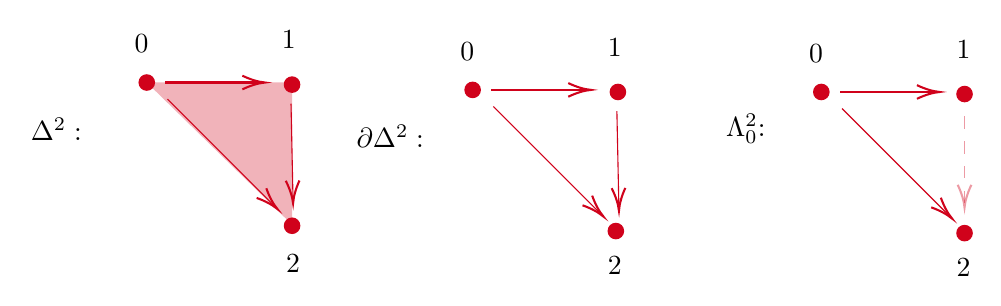
\begin{tikzpicture}[x=0.75pt,y=0.75pt,yscale=-1,xscale=1]
%uncomment if require: \path (0,240); %set diagram left start at 0, and has height of 240
%Shape: Free Drawing [id:dp20250857537916134] 
\draw  [color={rgb, 255:red, 208; green, 2; blue, 27 }  ,draw opacity=1 ][line width=6] [line join = round][line cap = round] (186.11,144.56) .. controls (186.11,144.56) and (186.11,144.56) .. (186.11,144.56) ;
%Shape: Free Drawing [id:dp8560192570653509] 
\draw  [color={rgb, 255:red, 208; green, 2; blue, 27 }  ,draw opacity=1 ][line width=6] [line join = round][line cap = round] (186.11,76.56) .. controls (186.11,76.56) and (186.11,76.56) .. (186.11,76.56) ;
%Shape: Free Drawing [id:dp26889850065743715] 
\draw  [color={rgb, 255:red, 208; green, 2; blue, 27 }  ,draw opacity=1 ][line width=6] [line join = round][line cap = round] (116.11,75.56) .. controls (116.11,75.56) and (116.11,75.56) .. (116.11,75.56) ;
%Straight Lines [id:da250770434621995] 
\draw [color={rgb, 255:red, 208; green, 2; blue, 27 }  ,draw opacity=1 ]   (185.61,85.78) -- (186.57,131.78) ;
\draw [shift={(186.61,133.78)}, rotate = 268.81] [color={rgb, 255:red, 208; green, 2; blue, 27 }  ,draw opacity=1 ][line width=0.75]    (10.93,-3.29) .. controls (6.95,-1.4) and (3.31,-0.3) .. (0,0) .. controls (3.31,0.3) and (6.95,1.4) .. (10.93,3.29)   ;
%Straight Lines [id:da5472503346326145] 
\draw [color={rgb, 255:red, 208; green, 2; blue, 27 }  ,draw opacity=1 ][line width=0.75]    (125.11,75.56) -- (171.11,75.56) ;
\draw [shift={(173.11,75.56)}, rotate = 180] [color={rgb, 255:red, 208; green, 2; blue, 27 }  ,draw opacity=1 ][line width=0.75]    (10.93,-3.29) .. controls (6.95,-1.4) and (3.31,-0.3) .. (0,0) .. controls (3.31,0.3) and (6.95,1.4) .. (10.93,3.29)   ;
%Straight Lines [id:da15503202104425817] 
\draw [color={rgb, 255:red, 208; green, 2; blue, 27 }  ,draw opacity=1 ]   (126.11,83.56) -- (177.7,135.14) ;
\draw [shift={(179.11,136.56)}, rotate = 225] [color={rgb, 255:red, 208; green, 2; blue, 27 }  ,draw opacity=1 ][line width=0.75]    (10.93,-3.29) .. controls (6.95,-1.4) and (3.31,-0.3) .. (0,0) .. controls (3.31,0.3) and (6.95,1.4) .. (10.93,3.29)   ;
%Shape: Polygon [id:ds5516763594874212] 
\draw  [draw opacity=0][fill={rgb, 255:red, 208; green, 2; blue, 27 }  ,fill opacity=0.3 ] (116.11,75.53) -- (186.11,75.53) -- (186.11,144.03) -- (116.11,75.53) -- cycle ;
%Shape: Free Drawing [id:dp6996632635597266] 
\draw  [color={rgb, 255:red, 208; green, 2; blue, 27 }  ,draw opacity=1 ][line width=6] [line join = round][line cap = round] (342.11,147.11) .. controls (342.11,147.11) and (342.11,147.11) .. (342.11,147.11) ;
%Shape: Free Drawing [id:dp23658558609305058] 
\draw  [color={rgb, 255:red, 208; green, 2; blue, 27 }  ,draw opacity=1 ][line width=6] [line join = round][line cap = round] (343.11,80.11) .. controls (343.11,80.11) and (343.11,80.11) .. (343.11,80.11) ;
%Shape: Free Drawing [id:dp5115039411399855] 
\draw  [color={rgb, 255:red, 208; green, 2; blue, 27 }  ,draw opacity=1 ][line width=6] [line join = round][line cap = round] (273.11,79.11) .. controls (273.11,79.11) and (273.11,79.11) .. (273.11,79.11) ;
%Straight Lines [id:da3744865515022133] 
\draw [color={rgb, 255:red, 208; green, 2; blue, 27 }  ,draw opacity=1 ]   (342.61,89.33) -- (343.57,135.33) ;
\draw [shift={(343.61,137.33)}, rotate = 268.81] [color={rgb, 255:red, 208; green, 2; blue, 27 }  ,draw opacity=1 ][line width=0.75]    (10.93,-3.29) .. controls (6.95,-1.4) and (3.31,-0.3) .. (0,0) .. controls (3.31,0.3) and (6.95,1.4) .. (10.93,3.29)   ;
%Straight Lines [id:da5413612535803476] 
\draw [color={rgb, 255:red, 208; green, 2; blue, 27 }  ,draw opacity=1 ][line width=0.75]    (282.11,79.11) -- (328.11,79.11) ;
\draw [shift={(330.11,79.11)}, rotate = 180] [color={rgb, 255:red, 208; green, 2; blue, 27 }  ,draw opacity=1 ][line width=0.75]    (10.93,-3.29) .. controls (6.95,-1.4) and (3.31,-0.3) .. (0,0) .. controls (3.31,0.3) and (6.95,1.4) .. (10.93,3.29)   ;
%Straight Lines [id:da17007192259087267] 
\draw [color={rgb, 255:red, 208; green, 2; blue, 27 }  ,draw opacity=1 ]   (283.11,87.11) -- (334.7,138.7) ;
\draw [shift={(336.11,140.11)}, rotate = 225] [color={rgb, 255:red, 208; green, 2; blue, 27 }  ,draw opacity=1 ][line width=0.75]    (10.93,-3.29) .. controls (6.95,-1.4) and (3.31,-0.3) .. (0,0) .. controls (3.31,0.3) and (6.95,1.4) .. (10.93,3.29)   ;
%Shape: Free Drawing [id:dp735452156887185] 
\draw  [color={rgb, 255:red, 208; green, 2; blue, 27 }  ,draw opacity=1 ][line width=6] [line join = round][line cap = round] (510.11,148.11) .. controls (510.11,148.11) and (510.11,148.11) .. (510.11,148.11) ;
%Shape: Free Drawing [id:dp12785217588086462] 
\draw  [color={rgb, 255:red, 208; green, 2; blue, 27 }  ,draw opacity=1 ][line width=6] [line join = round][line cap = round] (510.11,81.11) .. controls (510.11,81.11) and (510.11,81.11) .. (510.11,81.11) ;
%Shape: Free Drawing [id:dp4480432189571355] 
\draw  [color={rgb, 255:red, 208; green, 2; blue, 27 }  ,draw opacity=1 ][line width=6] [line join = round][line cap = round] (441.11,80.11) .. controls (441.11,80.11) and (441.11,80.11) .. (441.11,80.11) ;
%Straight Lines [id:da8320855200603781] 
\draw [color={rgb, 255:red, 208; green, 2; blue, 27 }  ,draw opacity=1 ][line width=0.75]    (450.11,80.11) -- (496.11,80.11) ;
\draw [shift={(498.11,80.11)}, rotate = 180] [color={rgb, 255:red, 208; green, 2; blue, 27 }  ,draw opacity=1 ][line width=0.75]    (10.93,-3.29) .. controls (6.95,-1.4) and (3.31,-0.3) .. (0,0) .. controls (3.31,0.3) and (6.95,1.4) .. (10.93,3.29)   ;
%Straight Lines [id:da24624276797536426] 
\draw [color={rgb, 255:red, 208; green, 2; blue, 27 }  ,draw opacity=1 ]   (451.11,88.11) -- (502.7,139.7) ;
\draw [shift={(504.11,141.11)}, rotate = 225] [color={rgb, 255:red, 208; green, 2; blue, 27 }  ,draw opacity=1 ][line width=0.75]    (10.93,-3.29) .. controls (6.95,-1.4) and (3.31,-0.3) .. (0,0) .. controls (3.31,0.3) and (6.95,1.4) .. (10.93,3.29)   ;
%Straight Lines [id:da36924497043702464] 
\draw [color={rgb, 255:red, 208; green, 2; blue, 27 }  ,draw opacity=0.4 ] [dash pattern={on 4.5pt off 4.5pt}]  (510.11,91.78) -- (510.11,133.78) ;
\draw [shift={(510.11,135.78)}, rotate = 270] [color={rgb, 255:red, 208; green, 2; blue, 27 }  ,draw opacity=0.4 ][line width=0.75]    (10.93,-3.29) .. controls (6.95,-1.4) and (3.31,-0.3) .. (0,0) .. controls (3.31,0.3) and (6.95,1.4) .. (10.93,3.29)   ;
% Text Node
\draw (59,91.4) node [anchor=north west][inner sep=0.75pt]    {$\Delta ^{2} :$};
% Text Node
\draw (109,51.4) node [anchor=north west][inner sep=0.75pt]    {$0$};
% Text Node
\draw (180,49.4) node [anchor=north west][inner sep=0.75pt]    {$1$};
% Text Node
\draw (182,157.4) node [anchor=north west][inner sep=0.75pt]    {$2$};
% Text Node
\draw (216,94.96) node [anchor=north west][inner sep=0.75pt]    {$\partial \Delta ^{2} :$};
% Text Node
\draw (266,54.96) node [anchor=north west][inner sep=0.75pt]    {$0$};
% Text Node
\draw (337,52.96) node [anchor=north west][inner sep=0.75pt]    {$1$};
% Text Node
\draw (337,157.96) node [anchor=north west][inner sep=0.75pt]    {$2$};
% Text Node
\draw (394,89.4) node [anchor=north west][inner sep=0.75pt]    {$\Lambda _{0}^{2}$:};
% Text Node
\draw (434,55.96) node [anchor=north west][inner sep=0.75pt]    {$0$};
% Text Node
\draw (505,53.96) node [anchor=north west][inner sep=0.75pt]    {$1$};
% Text Node
\draw (505,158.96) node [anchor=north west][inner sep=0.75pt]    {$2$};
\end{tikzpicture}\]
这解释了为什么说$\partial \Delta^n \simeq \bbS^{n-1}$.
此外,可以发现
\begin{proposition}\label{Pro:边界与尖角图表}
    单纯集范畴$\cate{sSet}$中有以下图表,上下两半分别交换($0\leq i < j \leq n$)
    \[\begin{tikzcd}
	{\Delta^{n-2}} & {\Delta^{n-1}} \\
	{\bigsqcup_{0\leq i' < j' \leq n}\Delta^{n-2}} & {\bigsqcup_{i'=0}^n\Delta^{n-1}} & {\partial\Delta^n} \\
	{\Delta^{n-2}} & {\Delta^{n-1}}
	\arrow["{\delta^{j-1}}", from=1-1, to=1-2]
	\arrow["{\iota_{i<j}}"', from=1-1, to=2-1]
	\arrow["{\iota_i}", from=1-2, to=2-2]
	\arrow["{\delta^i}", from=1-2, to=2-3]
	\arrow[shift left, from=2-1, to=2-2]
	\arrow[shift right, from=2-1, to=2-2]
	\arrow[from=2-2, to=2-3]
	\arrow["{\iota_{i<j}}", from=3-1, to=2-1]
	\arrow["{\delta^i}"', from=3-1, to=3-2]
	\arrow["{\iota_j}"', from=3-2, to=2-2]
	\arrow["{\delta^j}"', from=3-2, to=2-3]
    \end{tikzcd}\]
    其中$\bigsqcup$在$\cate{sSet}$中逐项选取,而$\iota_{i<j}$(或$\iota_i$)意谓向第$i<j$(或第$i$)项的嵌入;则有图表交换且中间部分为余等子.\\
    类似地,对$0\leq k \leq n$也有
    \[\begin{tikzcd}
	{\Delta^{n-2}} & {\Delta^{n-1}} \\
	{\bigsqcup_{0\leq i' < j' \leq n,i',j'\neq k}\Delta^{n-2}} & {\bigsqcup_{0\leq i'\leq n,i'\neq k}\Delta^{n-1}} & {\Lambda_k^n} \\
	{\Delta^{n-2}} & {\Delta^{n-1}}
	\arrow["{\delta^{j-1}}", from=1-1, to=1-2]
	\arrow["{\iota_{i<j}}"', from=1-1, to=2-1]
	\arrow["{\iota_i}", from=1-2, to=2-2]
	\arrow["{\delta^i}", from=1-2, to=2-3]
	\arrow[shift left, from=2-1, to=2-2]
	\arrow[shift right, from=2-1, to=2-2]
	\arrow[from=2-2, to=2-3]
	\arrow["{\iota_{i<j}}", from=3-1, to=2-1]
	\arrow["{\delta^i}"', from=3-1, to=3-2]
	\arrow["{\iota_j}"', from=3-2, to=2-2]
	\arrow["{\delta^j}"', from=3-2, to=2-3]
    \end{tikzcd}\]
    中间项也为余等子.
\end{proposition}
\begin{proof}
    验证即可.
\end{proof}
我们也可以将其视为$\partial \Delta^n$和$\Lambda_k^n$在``流水线''上的拼装过程,当然我们可以将其等价地表述为:
\begin{corollary}\label{推论:尖角变体}
    令$0 \leq i \leq n$为整数且$n >0$对于任意单纯集$S$,态射
    \begin{align*}
        \Hom_{\cate{sSet}}(\Lambda_k^n , S) &\to (S_{n-1})^n\\
        f &\mapsto \{f\circ \delta_n^j\}_{0\leq j \leq n,j \neq i}
    \end{align*}
    为单射,其像为``不完全''序列
    \[
        (\sigma_0,\cdots,\sigma_{i-1},\bullet,\sigma_{i+1},\cdots,\sigma_n)
    \]
    对于$k\in [n] \setminus \{i\}$且$j <k$的$k$ ,它满足等式$d_{n-1}^j(\sigma_k) = d_{n-1}^{k-1}(\sigma_j)$.
\end{corollary}
接下来引入脊(spine)的概念,它的意义将在后文得到阐述.
\begin{definition}[脊]
    对于$n$-单形$\Delta^n$定义子函子$I^n$为
    \[
    I^n := \{f\in \Hom([m],[n]): \Image(f) = \{j\} \text{或} \{j,j+1\}\}
    \]
\end{definition}
当$n=3$时$I^3 \subset \Delta^3$如下图所示,其中绿色虚线以及顶点为脊.
\[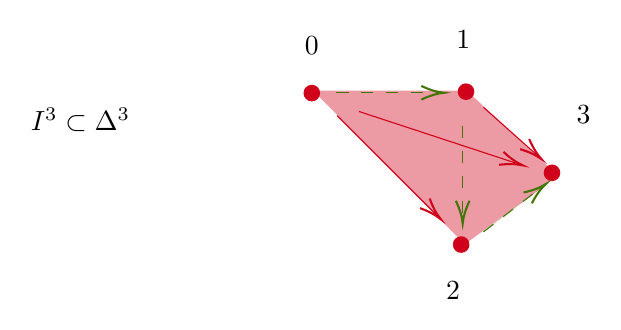
\begin{tikzpicture}[x=0.75pt,y=0.75pt,yscale=-1,xscale=1]
%uncomment if require: \path (0,184); %set diagram left start at 0, and has height of 184
%Straight Lines [id:da5832294719294788] 
\draw [draw opacity=0][fill={rgb, 255:red, 208; green, 2; blue, 27 }  ,fill opacity=0.4 ]   (317.33,62.5) -- (391.33,62.5) -- (435.33,103.5) -- (390.33,136.5) -- cycle ;
%Shape: Free Drawing [id:dp830584580009414] 
\draw  [color={rgb, 255:red, 208; green, 2; blue, 27 }  ,draw opacity=1 ][line width=6] [line join = round][line cap = round] (388.58,136.63) .. controls (388.58,136.63) and (388.58,136.63) .. (388.58,136.63) ;
%Shape: Free Drawing [id:dp3250839402586416] 
\draw  [color={rgb, 255:red, 208; green, 2; blue, 27 }  ,draw opacity=1 ][line width=6] [line join = round][line cap = round] (390.92,62.97) .. controls (390.92,62.97) and (390.92,62.97) .. (390.92,62.97) ;
%Shape: Free Drawing [id:dp7792822085041697] 
\draw  [color={rgb, 255:red, 208; green, 2; blue, 27 }  ,draw opacity=1 ][line width=6] [line join = round][line cap = round] (316.62,63.65) .. controls (316.62,63.65) and (316.62,63.65) .. (316.62,63.65) ;
%Shape: Free Drawing [id:dp19290457052024812] 
\draw  [color={rgb, 255:red, 208; green, 2; blue, 27 }  ,draw opacity=1 ][line width=6] [line join = round][line cap = round] (432.34,102.07) .. controls (432.34,102.07) and (432.34,102.07) .. (432.34,102.07) ;
%Straight Lines [id:da8563690958739549] 
\draw [color={rgb, 255:red, 65; green, 117; blue, 5 }  ,draw opacity=1 ] [dash pattern={on 4.5pt off 4.5pt}]  (328.33,63.5) -- (378.33,63.5) ;
\draw [shift={(380.33,63.5)}, rotate = 180] [color={rgb, 255:red, 65; green, 117; blue, 5 }  ,draw opacity=1 ][line width=0.75]    (10.93,-3.29) .. controls (6.95,-1.4) and (3.31,-0.3) .. (0,0) .. controls (3.31,0.3) and (6.95,1.4) .. (10.93,3.29)   ;
%Straight Lines [id:da6779286954756674] 
\draw [color={rgb, 255:red, 65; green, 117; blue, 5 }  ,draw opacity=1 ] [dash pattern={on 4.5pt off 4.5pt}]  (389.33,79.5) -- (389.33,124.5) ;
\draw [shift={(389.33,126.5)}, rotate = 270] [color={rgb, 255:red, 65; green, 117; blue, 5 }  ,draw opacity=1 ][line width=0.75]    (10.93,-3.29) .. controls (6.95,-1.4) and (3.31,-0.3) .. (0,0) .. controls (3.31,0.3) and (6.95,1.4) .. (10.93,3.29)   ;
%Straight Lines [id:da11968731710575464] 
\draw [color={rgb, 255:red, 65; green, 117; blue, 5 }  ,draw opacity=1 ][fill={rgb, 255:red, 65; green, 117; blue, 5 }  ,fill opacity=1 ] [dash pattern={on 4.5pt off 4.5pt}]  (399.33,130.5) -- (427.75,108.72) ;
\draw [shift={(429.33,107.5)}, rotate = 142.52] [color={rgb, 255:red, 65; green, 117; blue, 5 }  ,draw opacity=1 ][line width=0.75]    (10.93,-3.29) .. controls (6.95,-1.4) and (3.31,-0.3) .. (0,0) .. controls (3.31,0.3) and (6.95,1.4) .. (10.93,3.29)   ;
%Straight Lines [id:da17854575492651437] 
\draw [color={rgb, 255:red, 208; green, 2; blue, 27 }  ,draw opacity=1 ]   (328.83,74.5) -- (377.42,123.09) ;
\draw [shift={(378.83,124.5)}, rotate = 225] [color={rgb, 255:red, 208; green, 2; blue, 27 }  ,draw opacity=1 ][line width=0.75]    (10.93,-3.29) .. controls (6.95,-1.4) and (3.31,-0.3) .. (0,0) .. controls (3.31,0.3) and (6.95,1.4) .. (10.93,3.29)   ;
%Straight Lines [id:da8010680531974725] 
\draw [color={rgb, 255:red, 208; green, 2; blue, 27 }  ,draw opacity=1 ]   (339.33,72.5) -- (416.43,97.87) ;
\draw [shift={(418.33,98.5)}, rotate = 198.22] [color={rgb, 255:red, 208; green, 2; blue, 27 }  ,draw opacity=1 ][line width=0.75]    (10.93,-3.29) .. controls (6.95,-1.4) and (3.31,-0.3) .. (0,0) .. controls (3.31,0.3) and (6.95,1.4) .. (10.93,3.29)   ;
%Straight Lines [id:da06053624340237218] 
\draw [color={rgb, 255:red, 208; green, 2; blue, 27 }  ,draw opacity=1 ]   (399.33,70.5) -- (425.84,94.17) ;
\draw [shift={(427.33,95.5)}, rotate = 221.76] [color={rgb, 255:red, 208; green, 2; blue, 27 }  ,draw opacity=1 ][line width=0.75]    (10.93,-3.29) .. controls (6.95,-1.4) and (3.31,-0.3) .. (0,0) .. controls (3.31,0.3) and (6.95,1.4) .. (10.93,3.29)   ;
% Text Nod
\draw (385,32.4) node [anchor=north west][inner sep=0.75pt]    {$1$};
% Text Node
\draw (312,35.4) node [anchor=north west][inner sep=0.75pt]    {$0$};
% Text Node
\draw (443,68.4) node [anchor=north west][inner sep=0.75pt]    {$3$};
% Text Node
\draw (380.02,153.17) node [anchor=north west][inner sep=0.75pt]    {$2$};
% Text Node
\draw (180,69.4) node [anchor=north west][inner sep=0.75pt]    {$I^{3} \subset \Delta ^{3}$};
\end{tikzpicture}\]
不难发现$I^0 = \Delta^0$, $I^1 = \Delta^1$,且$I^n \subset \Lambda_i^n \subset \partial \Delta^n \subset \Delta^n$($1\leq i\leq n-1$或$n >3$).以及以下堆叠结构
\[
I^n = I^{n-1} \dsqcup{\Delta^0}\Delta^1.
\]
\section{单纯集的乘积}
\subsection{闭幺半范畴与$\cate{CGWH}$}\label{闭幺半与CGWH}
\begin{wenxintishi}
    为后文更加便利的叙述无穷范畴,我们来进行一点点题外话的讨论,这也是\parencite[Remark 1.1.1.7]{HTT}的更加详细的解释,不感兴趣的读者可以跳过.
\end{wenxintishi}
首先介绍闭幺半范畴的概念,不难发现单形对象可以和幺半范畴相联系.
\begin{definition}\label{Def:单形对象与幺半范畴}
    任何函子$F : \mathcal{C} \to \mathcal{D}$都相应地诱导$\mathsf{s}\mathcal{C}\to \mathsf{s}\mathcal{D}$,映资料$(X_n,d_i,s_j)_{n,i,j}$为$(FX_n,Fd_i,Fs_j)_{n,i,j}$.此外,有自明的关系式$\mathsf{s}(\mathcal{C}_1\times\mathcal{C}_2)\simeq {\mathsf{s}\mathcal{C}_1}\times{\mathsf{s}\mathcal{C}_2}$.\\
    将上述观察施于幺半范畴$\mathcal{C}$和双函子$\otimes:\mathcal{C}\times\mathcal{C} \to \mathcal{C}$,则对任意$X,Y\in \Obj(\mathsf{s}\mathcal{C})$可定义$X\otimes Y \in \Obj(\mathsf{s}\mathcal{C})$,其$n$次项为$X_n\otimes Y_n$,其面态射与退化态射分别形如$d_i \otimes d_j$和$s_i \otimes s_j$.
\end{definition}
\begin{definition}[闭幺半范畴]
    设$\mathcal{C}$为幺半范畴.当以下条件成立时,称$\mathcal{C}$为右(或左)闭幺半范畴:对所有对象$Y$,函子$ - \otimes Y : \mathcal{C} \to \mathcal{C}$(或$Y\otimes - : \mathcal{C} \to \mathcal{C}$)带有指定的右伴随.兼具左闭和右闭的幺半范畴称为闭幺半范畴.
\end{definition}
\begin{remark}
    我们考虑的幺半范畴均为辫幺半范畴,因此无需区分左闭右闭,此时$- \otimes Y$的右伴随记为$\underline{\Hom}(Y,-)$.
\end{remark}
一般而言,对任意范畴$\mathcal{C}_1$和$\mathcal{C}_2$之间的两对伴随函子$(F,G)$和$(F',G')$,任何$\varphi :F \to F'$都自然诱导了$\psi : G' \to G$.相反也是如此.诱导态射由交换图表
\[\begin{tikzcd}
	{\Hom(F'X,Y)} & {\Hom(X,G'Y)} \\
	{\Hom(FX,Y)} & {\Hom(X,GY)}
	\arrow["\sim"', from=1-1, to=1-2]
	\arrow["{(\varphi_X)^*}", from=1-1, to=2-1]
	\arrow["{(\psi_Y)_*}"', from=1-2, to=2-2]
	\arrow["\sim", from=2-1, to=2-2]
\end{tikzcd}\]
刻画.\\

作为应用,闭幺半范畴中的任何态射$Y \to Y'$诱导$\underline{\Hom}(Y', -)\to \underline{\Hom}(Y, -)$,所以闭幺半范畴的性质相当于在说存在双函子$\underline{\Hom}(-,-):\mathcal{C}^{\opposite} \times \mathcal{C} \to \mathcal{C}$以及一族典范双射
\begin{equation}\label{公式:内 Hom}
\tag{内 Hom}
   \Hom(X\otimes Y,Z) \simeq \Hom\left(X,\underline{\Hom}(Y,Z)\right), 
\end{equation}

它对于三个变元皆有函子性.\\

双函子$\underline{\Hom}(-,-)$也称为闭幺半范畴$\mathcal{C}$的内Hom.定义导致以下结论:
\begin{itemize}
    \item $\Hom(X,Z) \simeq \Hom(X\otimes \one,Z) \simeq \Hom(X,\underline{\Hom}(\one,Z))$,再由米田引理可知$Z \simeq \underline{\Hom}(\one,Z)$.
    \item 伴随对的单位态射给出$\coev_{X,Y}:X\to  \underline{\Hom}(Y,X\otimes Y)$,余单位态射给出$\ev_{Y,X}:\underline{\Hom}(Y,X)\otimes Y \to X$.
    \item 从合成
    \[\underline{\Hom}(Y,Z)\otimes(\underline{\Hom}(X,Y)\otimes X) \xrightarrow{\identity\otimes\ev_{X,Y}}\underline{\Hom}(Y,Z)\otimes Y\xrightarrow{\ev_{Y,Z}}Z\]
    以及伴随性质和结合约束可得
    \[
    \underline{\Hom}(Y,Z)\otimes\underline{\Hom}(X,Y)\to \underline{\Hom}(X,Z).
    \]
    \item 取$\coev_{\one,X}$得$\one \to \underline{\Hom}(X,X)$.
\end{itemize}
不难得到
\begin{proposition}
    设$\mathcal{C}$是闭幺半范畴,则有一族典范双射
    \[
    \Hom(X,Y) \simeq \Hom(\one,\underline{\Hom}(X,Y)),\quad X,Y \in \Obj(\mathcal{C}).
    \]
\end{proposition}
这说明内Hom可以得到Hom.\\

此外,伴随也可以内化到$\mathcal{C}$.
\begin{proposition}
    设$\mathcal{C}$是闭幺半范畴,则有一族同构
    \[
    \underline{\Hom}(X\otimes Y,Z)\simeq \underline{\Hom}(X,\underline{\Hom}(Y,Z));
    \]
    更精确地说,这是从$\mathcal{C}^{\opposite}\times \mathcal{C}^{\opposite}\times \mathcal{C} \to \mathcal{C}$的函子间的同构.
\end{proposition}
\begin{proof}
    考虑$\Hom(T,\underline{\Hom}(X\otimes Y,Z))$利用结合约束以及伴随同构证明$\Hom(T,\underline{\Hom}(X\otimes Y,Z))\rightiso \Hom(T,\underline{\Hom}(X,\underline{\Hom}(Y,Z)))$结合Yoneda引理可知结果.
\end{proof}
引入闭幺半范畴是为了进一步约化到双函子$\otimes$为积$\times$的情况,在这一情况下,会增加一个有趣的观察.
\begin{definition}[Cartesius闭]
    设$\mathcal{C}$是具备有限积的范畴.如果$(\mathcal{C},\times)$为闭幺半范畴,则称$\mathcal{C}$为Cartesius闭的.
\end{definition}
\begin{example}
\begin{enumerate}
    \item 集合范畴$\Set$是Cartesius闭的:取$\underline{\Hom}(X,Y) = Y^X$即可.
    \item 取$\mathcal{C} = \cate{Top}$,它具有许多良好性质,并且对积$\times$构成对称幺半范畴,但是它不是 Cartesian 闭的.
    \item 考虑全体小范畴构成的范畴$\cate{Cat}$,其中积为$\cal{C}_1\times \cdots \cal{C}_n$,而空积为$\bold{1}$.范畴$\cate{Cat}$是 Cartesian 闭的,这来自于以下简单的论断:指定双函子$\cal{A} \times \cal{B} \to \cal{C}$相当于指定函子$\cal{A} \to \cal{C}^{\cal{B}}$也相当于指定函子$\cal{B} \to \cal{C}^{\cal{A}}$.
\end{enumerate}
\end{example}
由于映射空间在拓扑学中俯拾即是,为解决$\cate{Top}$不是 Cartesian 闭的问题,我们引入紧生成空间与紧生成弱 Hausdorff 空间.两者都是方便的空间范畴,在$\infty$-范畴理论中,使用紧生成弱 Hausdorff 空间更多一些.\\
首先,回顾一下紧生成空间的定义,根据Bourbaki的定义,紧空间意谓紧且Hausdorff的空间.
\begin{definition}[弱Hausdorff]\label{定义:弱Hausdorff}
    设$X$为拓扑空间, $K$为紧空间,若对于任意连续映射$f: K \to X$都有$f(K)$是$X$中的闭集,则称$X$是弱Hausdorff的.
\end{definition}
\begin{example}
    Hausdorff空间是弱 Hausdorff 的.
\end{example}
这种空间的分离性介于T$_1$与Hausdorff之间.
\begin{definition}[紧闭子空间]\label{定义:紧闭子空间}
    设$X$为拓扑空间, $A \subset X$为其子空间, $K$为紧空间,若对于任意映射$f : K \to X$都有$f^{-1}(A)$为$K$中的闭集,则称$A$是$X$的紧闭子空间.\footnote{注意,不一定在$X$上闭}
\end{definition}
\begin{definition}[Kelly空间]
    设$X$为拓扑空间,若其每个紧闭子空间在$X$上都是闭的,则称$X$为Kelly空间,简称$k$-空间.
\end{definition}
\begin{definition}[紧生成空间]\label{定义:紧生成空间}
    设$X$为拓扑空间,以$X$中的紧闭子集作为闭集构成一个新的拓扑空间$kX$,有恒等映射$kX \to X$.若$kX = X$,则称$X$是紧生成的.记$\cate{CG}$为$\cate{Top}$中所有紧生成空间构成的范畴,当然也可以说是$k$-空间构成的范畴.
\end{definition}
\begin{proposition}\label{命题:紧生成化与嵌入函子伴随}
    由$X \mapsto kX$给出的函子$k : \cate{Top} \to \cate{CG}$是嵌入函子$\iota: \cate{CG} \to \cate{Top}$的右伴随.
\end{proposition}
\begin{proof}
    记$X \in \cate{CG}$, $Y\in \cate{Top}$,欲证
    \[
    \Hom_{\cate{CG}}(X,kY)\simeq \Hom_{\cate{Top}}(\iota X,Y),
    \]
    只需证明$f : X \to Y$连续当且仅当$f : X \to kY$连续即可.
    \begin{enumerate}
        \item[($\Rightarrow$)]假设$f: X\to Y$连续,则令$Z \subset Y$为紧闭子集考虑$f^{-1}(Z)$.对任意紧空间$K$,映射$g: K \to X$,由于$f\circ g : K \to Y$,因此$(f\circ g)^{-1}(Z)$在$K$中是闭的,这意味着$f^{-1}(Z)$为$X$中的紧闭子集,而$X$为紧生成空间,即$f^{-1}(Z)$在$X$中闭,从而$kY$中的闭集在$f$的逆像为$X$中的闭集从而$f: X \to kY$连续.
        \item[($\Leftarrow$)]由于$kY \to Y$连续,因此考虑复合即可.
    \end{enumerate}
\end{proof}
\begin{proposition}\label{Pro:紧生成空间商映射}
    若$X \in \cate{CG}$, $\pr: X\to Y$为商映射,则$Y\in \cate{CG}$.
\end{proposition}
\begin{proof}
    由于商映射为使得$\pr : X \to Y$连续的最细的映射且有分解$\pr : X \to kY \to Y$,因此$Y = kY$.
\end{proof}
\begin{theorem}[$\cate{CG}$的完备性]
    范畴$\cate{CG}$完备且余完备.其余极限继承相应空间在$\cate{Top}$中的余极限,而极限由$k$作用于相应空间在$\cate{Top}$中的极限得到.
\end{theorem}
\begin{proof}
    设$\mathcal{I}$为指标范畴, $F \in \Fct(\mathcal{I},\cate{CG})$, $\hat{F} = \iota \circ F$.由于$\iota$为左伴随,保$\indlim$,因此只需要证明$\cate{CG}$中对象在$\cate{Top}$的余极限仍在$\cate{CG}$中即可,由于命题\ref{Pro:紧生成空间商映射},只需要证明$\bigsqcup_{i\in \mathcal{I}}F(i)$在$\cate{CG}$中即可,这是显然的.而后由于$k$为右伴随,因此保$\prolim$,即
    \[
    \underset{i\in \mathcal{I}}{\prolim} F(i) = \underset{i\in \mathcal{I}}{\prolim} (k\circ \hat{F}(i)) = k \underset{i\in \mathcal{I}}{\prolim} \hat{F}(i).
    \]
\end{proof}
\begin{corollary}
    令$\{X_i\}_{i\in I}$为$\cate{CG}$中的一族对象.则它们在$\cate{CG}$中的乘积为
    \[
     k(\prod_{i\in I}X_i)
    \]
    此处$\prod_{i\in I}X_i$为在拓扑空间中的乘积.
\end{corollary}
\begin{definition}[紧生成弱Hausdorff空间]\label{Def:紧生成弱Hausdorff空间}
    设$X$为拓扑空间,若其是弱Hausdorff的$k$-空间,则称其为紧生成空间,其构成的范畴记为$\cate{CGWH}$.
\end{definition}
\begin{example}
    引理\ref{Lem:单纯集几何实现与CW-复形}可知$|\cate{sSet}| \subset \cate{CGWH}$.
\end{example}
\begin{proposition}
    设$X$为弱Hausdorff空间, $K$为紧空间,若$f : K \to X$连续,则$f(K)$为紧空间.
\end{proposition}
\begin{proof}
    由于$K$紧且$X$弱Hausdorff,由定义即知$f(K)$闭,而由连续映射保持紧性知$f(K)$紧,此外得知$f$为闭映射.而后考虑$x_1,x_2 \in f(K)$由于$X$为弱Hausdorff空间, $\{x_1\}$和$\{x_2\}$为闭子集,因此考虑其逆像得知$f^{-1}(x_1)$与$f^{-1}(x_2)$无交,而$K$紧Hausdorff,从而存在$U_1,U_2$为$K$中开集使得$f^{-1}(x_1)\in U_1$而$f^{-1}(x_2)\in U_2$,即$x_2\in K-U_1$而$x_1 \in K-U_2$.考虑$f(K) - f(K-U_i)$($i=1,2$)便得到包含$x_1$和$x_2$的无交开集.
\end{proof}
\begin{proposition}
    设$X$为紧生成空间,则$X$弱Hausdorff当且仅当对角线子空间$\delta_X$在$X\times X$中闭,此处$X \times X$为$\cate{CG}$中的乘积.
\end{proposition}
\begin{proof}
    设$X \in  \cate{CGWH}$,现证$\delta_X$紧闭.考虑
    \[
    f=(f_1,f_2) : K \to X\times X, f_i : K \to X
    \]
    $K$为紧空间,记
    \[
    L = f_1(K) \cap f_2(K)
    \]
    可知$L$为紧空间.考虑对角线$\delta_L$,由于$L$为紧空间, $\delta_L$为$X\times X$的紧子空间,而$X$紧生成,因此$\delta_L$在$X\times X$中闭.即$f^{-1}(\delta_X) = f^{-1}(\delta_L)$闭.\\
    反过来只需证明若$K$为紧空间$f: K\to X$连续,则$f(K)$紧闭即可.不妨设$L$为紧空间, $g: L \to X$连续,考虑
    \[
    (f,g): K \times L \to X\times X.
    \]
    则
    \[
    g^{-1}(f(K)) = (f,g)^{-1}(\delta_X)
    \]
    为闭集,即$f(K)$紧闭.
\end{proof}
\begin{corollary}\label{Cor:CG乘积也在CGWH中}
    设$\{X_i\}$为$\cate{CGWH}$中的一族对象,则它们在$\cate{CG}$的乘积也在$\cate{CGWH}$中.
\end{corollary}
\begin{proposition}
    函子$h : \cate{CG} \to \cate{CGWH}$是嵌入$\iota': \cate{CGWH}\to \cate{CG}$的左伴随.
\end{proposition}
\begin{theorem}[$\cate{CGWH}$的完备性]\label{The:CGWH的完备性}
    范畴$\cate{CGWH}$完备且余完备.极限继承自$\cate{CG}$而余极限来自$h$作用于$\cate{CG}$.
\end{theorem}
\begin{proof}
    与$\cate{CG}$完备且余完备的证明是类似的.唯一不平凡的是需要使用推论\ref{Cor:CG乘积也在CGWH中}即可得知乘积存在,而后由范畴中构造极限的方式可以证明极限确实继承自$\cate{CG}$.
\end{proof}
\begin{proposition}
    $\cate{CGWH}$是 Cartesian 闭的.
\end{proposition}
\begin{proof}   
见\parencite[Proposition 2.12]{StricklandCGWH}
\end{proof}
在对于同伦论的研究中,使用紧生成弱Hausdorff空间范畴$\cate{CGWH}$是更加方便的.因为$\cate{Top}$不是Cartesius闭的\footnote{由于不保\href{https://ncatlab.org/nlab/show/regular+epimorphism}{正则满态射(regular epimorphism)}},而\begin{tikzcd}
	{\cate{CGWH}} & {\cate{Top}}
	\arrow["{\text{包含}}", shift left, from=1-1, to=1-2]
	\arrow["k", shift left, from=1-2, to=1-1]
    \end{tikzcd}
中$\cate{CGWH}$为Cartesius闭范畴;可以证明前文伴随对中包含函子保$\indlim$但不保积.由于前文中$n$-单纯集的几何实现$|\Delta^n|$是一个紧生成弱Hausdorff空间,并且,因此几何实现(或奇异集)中的粘合(或取$\Hom$)可在$\cate{CGWH}$中操作(因所论的极限都在$\cate{CGWH}$中存在)因此定理\ref{The:几何实现是奇异集函子的左伴随}中伴随对分为两段
\[\begin{tikzcd}
	{\cate{sSet}} & {\cate{CGWH}} & {\cate{Top}}
	\arrow["{|-|}", shift left, from=1-1, to=1-2]
	\arrow["\Sing", shift left, from=1-2, to=1-1]
	\arrow["{\text{包含}}", shift left, from=1-2, to=1-3]
	\arrow["k", shift left, from=1-3, to=1-2]
\end{tikzcd}\]
对任意两个单纯集$X$和$Y$,就可以定义它们的逐项积
\begin{align*}
    (X\times Y)_n &= X_n \times Y_n\\
    d_i(x,y) &= (d_i(x),d_i(y))\\
    s_j(x,y) &= (s_j(x),s_j(y)).
\end{align*}
这是定义\ref{Def:单形对象与幺半范畴}中取$(\cate{Set},\times)$的产物,以下结果表明其承载几何意义.
\begin{theorem}\label{The:单纯集的积的几何意义}
    对于单纯集$X$和$Y$,我们有$\cate{CGWH}$中的典范同构
    \[
    |X\times Y| \simeq |X|\times |Y|
    \]
    推而广之, $\cate{CGWH}$版本的$|-|$保有限$\prolim$.若$X$和$Y$其中之一仅有有限多个非退化单纯形,则$|X\times Y| \simeq |X|\times |Y|$在$\cate{Top}$中也成立.
\end{theorem}
\begin{proof}
    在\parencite[Chapter 3, $\S$3,(3.1)]{Gabriel-Zisman67}中已经证明几何实现与余极限以及有限极限可交换而后在\parencite[Chapter 3, $\S$3,(3.5)]{Gabriel-Zisman67}中说明对于任意单纯集$X,Y$都有
    \[
    |X \times Y| \rightiso k(|X| \times |Y|)
    \]
    因此在$\cate{CGWH}$中有典范同构
    \[
    |X \times Y| \rightiso |X| \times |Y|
    \]
\end{proof}
\begin{remark}
    事实上,我们有\href{https://ncatlab.org/nlab/show/convenient+category+of+topological+spaces}{方便的空间范畴(convenient category of topological spaces)}一说.
\end{remark}
\begin{corollary}
    记$\cate{Grp}$,若单纯形集$X$可以升级为$\cate{Grp}^{\Delta^{\opposite}}$的对象,则$|X|$也自然地具有拓扑群结构;对于其它代数结构也有类似的结果.
\end{corollary}
在单纯集中,结合定理\ref{The:单纯集的积的几何意义}可以很自然地定义出同伦来,对于$\cate{sSet}$中的态射$f,g : X \twoheadrightarrow Y$定义$g$到$f$的(单纯)同伦为态射$H: X\times \Delta^1 \to Y$,使得下图交换:
\[\begin{tikzcd}
	{X\times \Delta^0} && X \\
	{X\times \Delta^1} && Y \\
	{X\times \Delta^0} && X
	\arrow["\sim", from=1-1, to=1-3]
	\arrow["{\identity_X \times d_0}"', from=1-1, to=2-1]
	\arrow["f"{description}, from=1-3, to=2-3]
	\arrow["H"{description}, from=2-1, to=2-3]
	\arrow["{\identity_X\times d_1}", from=3-1, to=2-1]
	\arrow["\sim"', from=3-1, to=3-3]
	\arrow["g"{description}, from=3-3, to=2-3]
\end{tikzcd}\]
熟悉模型范畴的读者应当可以看出此处\href{https://ncatlab.org/nlab/show/homotopy+in+a+model+category}{同伦}为使用\href{https://ncatlab.org/nlab/show/cylinder+object}{柱对象}定义的左同伦,自然也有使用\href{https://ncatlab.org/nlab/show/path+space+object}{路径对象}\footnote{柱对象和路径对象分别模仿$X \times I\to Y$和$X \to Y^I$两种情况.}所定义出的右同伦(或称余单纯同伦)$F : X \to Y^{\Delta^1}$,使得下图交换:
\[\begin{tikzcd}
	Y && {Y^{\Delta^0}} \\
	X && {Y^{\Delta^1}} \\
	Y && {Y^{\Delta^0}}
	\arrow["\sim", from=1-3, to=1-1]
	\arrow["f"', from=2-1, to=1-1]
	\arrow["F"{description}, from=2-1, to=2-3]
	\arrow["g", from=2-1, to=3-1]
	\arrow["{(d_1)^*}", from=2-3, to=1-3]
	\arrow["{(d_0)^*}"', from=2-3, to=3-3]
	\arrow["\sim"', from=3-3, to=3-1]
\end{tikzcd}\]

可以证明在拟范畴中这两种同伦是一致的,具有关心左右同伦及其一致性雅兴的读者,敬请阅读\parencite[11.4 and 11.7]{RezkQuasi-Cat}.\\
最后,我们探讨$\cate{sSet}$的 Cartesian 闭性.
\begin{definition}
    对于 $X,Y\in \Obj(\cate{sSet})$, 定义$\Fct(X,Y) = \iHom_{\cate{sSet}}(X,Y)\in \Obj(\cate{sSet})$如下
    \[
    \Fct(X,Y)_n := \Hom_{\cate{sSet}}(X\times \Delta^n,Y),\quad n\in \Z_{\geq 0},
    \]
    而对$\Delta$的任意态射$f: [m]\to [n]$,定义$f^* : \Fct(X,Y)_m \to \Fct(X,Y)_n$为沿
    \[
    \identity \times f : X \times \Delta^m \to X \times \Delta^n
    \]
    的拉回.另外,求值态射
    \[
    \ev_{X,Y}: \Fct(X,Y)\times X \to Y
    \]
    定义如下:$(\varphi,x)\in \Hom_{\cate{sSet}}(X\times \Delta^n,Y)_n\times X_n$的像为$\ev_{X,Y,n}(\varphi,x) := \varphi(x,\identity_{[n]})\in Y_n$(回忆到$(\Delta^n)_n = \Hom([n],[n]) = \End([n])$).
\end{definition}
必须验证$\ev_{X,Y}$确实是$\cate{sSet}$的态射.这毫不困难:给定$f: [m] \to [n]$和$(\varphi,x)\in \Fct(X,Y)_n \times X_n$,有
\begin{align*}
    \ev_{X,Y,m}(f^*(\varphi),f^*(x)) &= \left((\identity_X\times f)^*\varphi\right) \left(f^*(x),\identity_{[m]}\right)\\
    &= \varphi\left(\underset{\in X_m \times(\Delta^n)_m}{\underbrace{f^*(x),f}}\right) = \varphi\left(f^*(x),f^*\identity_{[n]}\right)\\
    &= f^*\left(\varphi(x,\identity_{[n]})\right) = f^*\left(\ev_{X,Y,n}(\varphi,x)\right).
\end{align*}
变动$X,Y$,给出函子$\Fct : \cate{sSet}^{\opposite}\times \cate{sSet} \to \cate{sSet}$而$\ev$对$X$和$Y$是典范的.
\begin{theorem}[$\cate{sSet}$是 Cartesian 闭的]\label{定理:sSet是Cartesian闭的}
    对所有$X,Y,Z\in \Obj(\cate{sSet})$,有典范双射
    \[
    \Hom_{\cate{sSet}}(X,\Fct(Y,Z))\xleftrightarrow{1:1} \Hom_{\cate{sSet}}(X\times Y,Z)
    \]
    它映$g:X \to \Fct(Y,Z)$为以下态射的合成
    \[
    X\times Y \xrightarrow{g\times \identity_{Y}}\Fct(Y,Z) \times Y \xrightarrow{\ev_{Y,Z}}Z.
    \]
    它映$h : X \times Y \to Z$为以下态射:设$n\in \Z_{\geq 0}$而$x\in X_n$,对应于态射$\iota_x : \Delta^n \to X$,则$x$的像是以下合成
    \[
    Y\times \Delta^n \xrightarrow{\identity_Y \times \iota_x}Y \times X\xrightarrow[\sim]{\text{换位}} X \times Y \xrightarrow{h} Z
    \]
    结合公式(\ref{公式:内 Hom})可判断$\cate{sSet}$是Cartesian闭的.
\end{theorem}
\begin{proof}
    验证即可.
\end{proof}
\subsection{标准单形的乘积}
接下来我们讨论$X = \Delta^p$和$Y = \Delta^q$时所对应的$\Delta^p \times \Delta^q$,比方说,如何分类$\Delta^p \times \Delta^q$上的非退化单形?问题的答案非但有助于理解积的几何实现,相关构造也是之后需要的.\\
首先,任两个偏序集$S_1$和$S_2$的积$S_1 \times S_2$通过$(a_1,a_2) \leq (b_1,b_2) \Leftrightarrow a_1 \leq b_1,a_2 \leq b_2$成为偏序集,这也相当于取它们对应范畴的积.
\begin{definition}
    设$p,q\in \Z_{\geq 0}$.所谓$(p,q)$-重组,意谓保序单射$\sigma : [p+q]\to [p]\times [q]$.
\end{definition}
对任意$n\in \Z_{\geq 0}$,指定保序映射$[n] \to [p]\times [q]$相当于指定一对保序映射$\sigma_{-} : [n] \to [p]$以及$\sigma_{+}:[n] \to [q]$;也相当于指定$\Delta^p \times \Delta^q$的一个$n$-单形.要求$i \mapsto (\sigma_{-}(i),\sigma_{+}(i))$的轨迹不停顿($i = 0,\cdots,n$).对于$n = p+q$时可以图解为
\[\begin{tikzpicture}[x=0.75pt,y=0.75pt,yscale=-1,xscale=1]
%uncomment if require: \path (0,300); %set diagram left start at 0, and has height of 300

%Shape: Square [id:dp9200085151915061] 
\draw  [color={rgb, 255:red, 155; green, 155; blue, 155 }  ,draw opacity=1 ] (127,81) -- (161.11,81) -- (161.11,115.11) -- (127,115.11) -- cycle ;
%Shape: Square [id:dp7316878376868328] 
\draw  [color={rgb, 255:red, 155; green, 155; blue, 155 }  ,draw opacity=1 ] (161.11,81) -- (195.22,81) -- (195.22,115.11) -- (161.11,115.11) -- cycle ;
%Shape: Square [id:dp7345201478772678] 
\draw  [color={rgb, 255:red, 155; green, 155; blue, 155 }  ,draw opacity=1 ] (127,115.11) -- (161.11,115.11) -- (161.11,149.22) -- (127,149.22) -- cycle ;
%Shape: Square [id:dp9194245889335557] 
\draw  [color={rgb, 255:red, 155; green, 155; blue, 155 }  ,draw opacity=1 ] (161.11,115.11) -- (195.22,115.11) -- (195.22,149.22) -- (161.11,149.22) -- cycle ;
%Shape: Square [id:dp9819463147507028] 
\draw  [color={rgb, 255:red, 155; green, 155; blue, 155 }  ,draw opacity=1 ] (195.22,81) -- (229.33,81) -- (229.33,115.11) -- (195.22,115.11) -- cycle ;
%Shape: Square [id:dp2144558429344554] 
\draw  [color={rgb, 255:red, 155; green, 155; blue, 155 }  ,draw opacity=1 ] (229.33,81) -- (263.44,81) -- (263.44,115.11) -- (229.33,115.11) -- cycle ;
%Shape: Square [id:dp03657410340992695] 
\draw  [color={rgb, 255:red, 155; green, 155; blue, 155 }  ,draw opacity=1 ] (263.44,81) -- (297.56,81) -- (297.56,115.11) -- (263.44,115.11) -- cycle ;
%Shape: Square [id:dp12006168557256958] 
\draw  [color={rgb, 255:red, 155; green, 155; blue, 155 }  ,draw opacity=1 ] (195.22,115.11) -- (229.33,115.11) -- (229.33,149.22) -- (195.22,149.22) -- cycle ;
%Shape: Square [id:dp1242866028192735] 
\draw  [color={rgb, 255:red, 155; green, 155; blue, 155 }  ,draw opacity=1 ] (229.33,115.11) -- (263.44,115.11) -- (263.44,149.22) -- (229.33,149.22) -- cycle ;
%Shape: Square [id:dp648778429497445] 
\draw  [color={rgb, 255:red, 155; green, 155; blue, 155 }  ,draw opacity=1 ] (263.44,115.11) -- (297.56,115.11) -- (297.56,149.22) -- (263.44,149.22) -- cycle ;
%Shape: Square [id:dp2740991741808232] 
\draw  [color={rgb, 255:red, 155; green, 155; blue, 155 }  ,draw opacity=1 ] (127,149.22) -- (161.11,149.22) -- (161.11,183.33) -- (127,183.33) -- cycle ;
%Shape: Square [id:dp37269635233617526] 
\draw  [color={rgb, 255:red, 155; green, 155; blue, 155 }  ,draw opacity=1 ] (161.11,149.22) -- (195.22,149.22) -- (195.22,183.33) -- (161.11,183.33) -- cycle ;
%Shape: Square [id:dp9507679799360924] 
\draw  [color={rgb, 255:red, 155; green, 155; blue, 155 }  ,draw opacity=1 ] (195.22,149.22) -- (229.33,149.22) -- (229.33,183.33) -- (195.22,183.33) -- cycle ;
%Shape: Square [id:dp5843515974208688] 
\draw  [color={rgb, 255:red, 155; green, 155; blue, 155 }  ,draw opacity=1 ] (229.33,149.22) -- (263.44,149.22) -- (263.44,183.33) -- (229.33,183.33) -- cycle ;
%Shape: Square [id:dp9355071433648059] 
\draw  [color={rgb, 255:red, 155; green, 155; blue, 155 }  ,draw opacity=1 ] (263.44,149.22) -- (297.56,149.22) -- (297.56,183.33) -- (263.44,183.33) -- cycle ;
%Shape: Square [id:dp8376323002057664] 
\draw  [color={rgb, 255:red, 155; green, 155; blue, 155 }  ,draw opacity=1 ] (127,183.33) -- (161.11,183.33) -- (161.11,217.44) -- (127,217.44) -- cycle ;
%Shape: Square [id:dp4248702782223266] 
\draw  [color={rgb, 255:red, 155; green, 155; blue, 155 }  ,draw opacity=1 ] (161.11,183.33) -- (195.22,183.33) -- (195.22,217.44) -- (161.11,217.44) -- cycle ;
%Shape: Square [id:dp9607310045186002] 
\draw  [color={rgb, 255:red, 155; green, 155; blue, 155 }  ,draw opacity=1 ] (195.22,183.33) -- (229.33,183.33) -- (229.33,217.44) -- (195.22,217.44) -- cycle ;
%Shape: Square [id:dp25732339354119693] 
\draw  [color={rgb, 255:red, 155; green, 155; blue, 155 }  ,draw opacity=1 ] (229.33,183.33) -- (263.44,183.33) -- (263.44,217.44) -- (229.33,217.44) -- cycle ;
%Shape: Square [id:dp23379818350891357] 
\draw  [color={rgb, 255:red, 155; green, 155; blue, 155 }  ,draw opacity=1 ] (263.44,183.33) -- (297.56,183.33) -- (297.56,217.44) -- (263.44,217.44) -- cycle ;
%Straight Lines [id:da7298797239711685] 
\draw [line width=1.5]    (127,217.44) -- (161.11,217.44) -- (161.11,183.33) -- (195.22,183.33) -- (229.33,183.33) -- (229.33,149.22) -- (263.44,149.22) -- (263.44,81) -- (297.56,81) ;

% Text Node
\draw (75,216.4) node [anchor=north west][inner sep=0.75pt]    {$i=0$};
% Text Node
\draw (309,61.4) node [anchor=north west][inner sep=0.75pt]    {$( p,q)$};
% Text Node
\draw (380,137) node [anchor=north west][inner sep=0.75pt]   [align=left] {恰好移动 $\displaystyle p+q$ 步};
\end{tikzpicture}\]
于是对于$(p,q)$-重组$\sigma$可以定义
\begin{align*}
    I_{\pm} &:= \{1\leq i \leq p+q : \sigma_{\pm}(i-1) < \sigma_{\pm}(i)\}\\
    &=\{1\leq i \leq p+q:\sigma_{\pm}(i-1) = \sigma_{\pm}(i)-1\}\\
    &=\{1\leq i \leq p+q:\sigma_{\mp}(i-1) = \sigma_{\mp}(i)\},
\end{align*}
它们满足$I_+ \sqcup I_- = \{1,\cdots,p+q\}$.子集$I_+$(或$I_-$)如上图的向上(或向右)部分,故$(p,q)$-重组的另一种观点是视其为$p$个$\to$以及$q$个$\uparrow$的排列,不难发现有${p+q}\choose{p}$种.这些观察顺带说明$\sigma_{+}$和$\sigma_{-}$对于$(p,q)$-重组是保序满射.
\begin{proposition}
    设$p,q\in \Z_{\geq 0}$.考虑$\Delta^p \times \Delta^q$的$n$-单形,亦即保序映射$\sigma : [n] \to [p]\times [q]$.命$(p_i,q_i):=\sigma(i)$, $(p',q'):= (p_n-p_0,q_n-q_0)$,则$\sigma$非退化当且仅当下述条件成立
    \begin{enumerate}
        \item $p'+q' = n$;
        \item $\sigma$分解为$(p',q')$-重组$\sigma' : [n] \to [p']+[q']$和形如$f\times g$的保序单射$[p']\times [q'] \hookrightarrow [p]\times [q]$.
    \end{enumerate}
\end{proposition}
\begin{proof}
    让$\sigma$对应到保序映射对$(\sigma_-,\sigma_+)$.不难发现$\sigma$非退化相当于说$i\mapsto (p_i,q_i)$的轨迹不停顿.因此命题是自明的.
\end{proof}
基于非退化单纯形的描述,读者不妨发挥想象力揣摩$|\Delta^p \times \Delta^q| \simeq |\Delta^p| \times |\Delta^q|$在$(p,q) =(1,1)$和$(2,1)$时的道理.例如下图是将$|\Delta^2 |\times |\Delta^1|$剖分为$3$个四面体的结果,对应于$3 = {3\choose 2}$个$(2,1)$-重组.
\[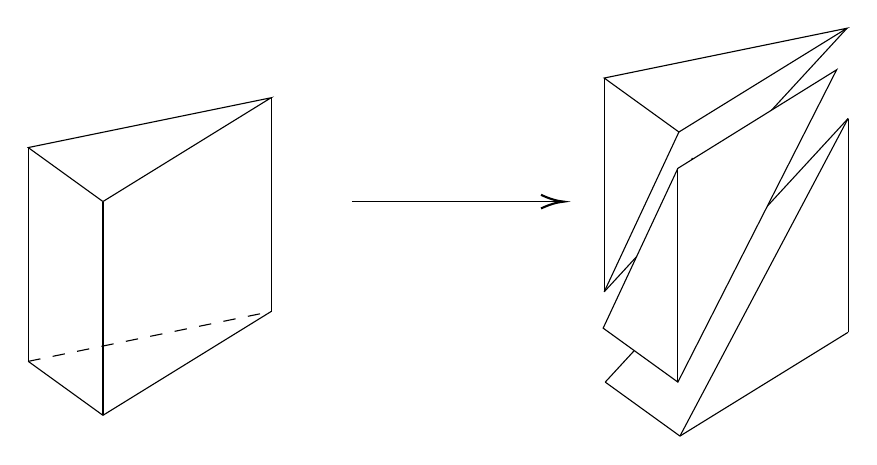
\begin{tikzpicture}[x=0.75pt,y=0.75pt,yscale=-1,xscale=1]
%uncomment if require: \path (0,300); %set diagram left start at 0, and has height of 300

%Straight Lines [id:da7320988534337254] 
\draw    (206.11,89.95) -- (89.11,113.95) -- (125.11,139.95) -- cycle ;
%Straight Lines [id:da7731734512646173] 
\draw    (89.11,113.95) -- (89.11,216.95) ;
%Straight Lines [id:da8693410695407291] 
\draw    (125.11,139.95) -- (125.11,242.95) ;
%Straight Lines [id:da34778996424608755] 
\draw    (206.11,89.95) -- (206.11,192.95) ;
%Straight Lines [id:da6485703140189338] 
\draw    (89.11,216.95) -- (125.11,242.95) -- (206.11,192.95) ;
%Straight Lines [id:da4428671688368293] 
\draw  [dash pattern={on 4.5pt off 4.5pt}]  (89.11,216.95) -- (206.11,192.95) ;
%Straight Lines [id:da6469878563000044] 
\draw    (245,140) -- (345.11,140) ;
\draw [shift={(347.11,140)}, rotate = 180] [color={rgb, 255:red, 0; green, 0; blue, 0 }  ][line width=0.75]    (10.93,-3.29) .. controls (6.95,-1.4) and (3.31,-0.3) .. (0,0) .. controls (3.31,0.3) and (6.95,1.4) .. (10.93,3.29)   ;
%Straight Lines [id:da9786602942081664] 
\draw    (366.61,80.45) -- (366.61,183.45) ;
%Straight Lines [id:da09611235081394187] 
\draw    (373.11,195.95) -- (409.11,118.95) ;
%Straight Lines [id:da03367413546565712] 
\draw    (402.61,106.45) -- (366.61,183.45) ;
%Straight Lines [id:da5015870642967339] 
\draw    (366.61,183.45) -- (483.61,56.45) ;
%Straight Lines [id:da8842588269678069] 
\draw    (483.61,56.45) -- (366.61,80.45) -- (402.61,106.45) -- cycle ;
%Straight Lines [id:da2697482316833171] 
\draw    (367.11,226.95) -- (403.11,252.95) -- (484.11,202.95) ;
%Straight Lines [id:da33617365628102003] 
\draw    (484.11,99.95) -- (484.11,202.95) ;
%Straight Lines [id:da782615014690863] 
\draw    (403.11,252.95) -- (484.11,99.95) ;
%Straight Lines [id:da3404844465403125] 
\draw    (367.11,226.95) -- (484.11,99.95) ;
%Shape: Polygon [id:ds9600948394944278] 
\draw  [fill={rgb, 255:red, 255; green, 255; blue, 255 }  ,fill opacity=1 ] (478.61,76.45) -- (402.11,226.95) -- (402.11,226.95) -- (366.11,200.95) -- (402.11,123.95) -- cycle ;
%Straight Lines [id:da037161638623682824] 
\draw    (402.11,123.95) -- (402.11,159.95) -- (402.11,226.95) ;
\end{tikzpicture}
\]
\begin{definition}
    设$\sigma$为$(p,q)$-重组,其符号定义为
    \[
    \sgn(\sigma) := (-1)^{|I_{\sigma}|}, I_{\sigma}:= \{(i,j) \in I_- \times I_+: i >j\}.
    \]
\end{definition}
    若将$\sigma$视同$p$个$\rightarrow$以及$q$个$\uparrow$的排列,则$I_{\sigma}$就是所有出现``错排''$(\uparrow,\rightarrow)$的数对$(j,i)$其中$j <i$.简单的组合学练习告诉我们存在唯一的$\tau \in \frak{S}_{p+q}$将这般排列还原为形如$\rightarrow\cdots\rightarrow\uparrow\cdots\uparrow$的样式,而不打乱$I_+$和$I_-$内部的顺序,而上述定义相当于说$\sgn(\sigma) = \sgn(\tau)$.\\
    对于$(p,q)$-重组$\sigma$,调换$\sigma_-$和$\sigma_+$的角色给出$(q,p)$-重组$\sigma'$.上述诠释和基本的组合学论证表明
    \[
    \sgn(\sigma) = (-1)^{pq}\sgn(\sigma')
    \]
    准此要领,类似地定义$(p,q,r)$-重组为保序单射$\sigma = (\sigma_-,\sigma_0,\sigma_+):[p+q+r] \to [p]\times [q]\times [r]$,或理解为三维空间中向右$\rightarrow$,向前$\nearrow$以及向上$\uparrow$的排列.同样的组合学练习表明若$(p,q,r)$-重组$\sigma$有分解\footnote{当然可以分解为$[p+q+r] \xrightarrow{\sigma_1}[p]\times [q+r]\xrightarrow{\identity_{[p]} \times \sigma_2}[p]\times[q]\times[r]$}
    \[
    [p+q+r] \xrightarrow{\sigma_1}[p+q]\times [r]\xrightarrow{\sigma_2 \times \identity_{[r]}}[p]\times[q]\times[r]
    \]
    则$\sigma_1$是$(p+q,r)$-重组,$\sigma_2$是$(p,q)$-重组,而且
    \[
    \sgn(\sigma) = \sgn(\sigma_1)\sgn(\sigma_2)
    \]
    由此可以给出$n$-重单形对象.今后,对$\Delta$的一族对象$[m_1],\cdots,[m_n]$,今后将$(\Delta)^n$中的对象$([m_1],\cdots,[m_n])$另记为$[m_1]\times \cdots \times [m_n]$以便排版.
    \begin{definition}
        设$\cal{C}$为任意范畴, $n\in \Z_{\geq 1}$. 形如$X : (\Delta^{\opposite})^n \to \cal{C}$(或$\Delta^n \to \cal{C}$)的函子称为$\cal{C}$中的$n$重单形对象(或$n$重余单形对象);态射理解为它们作为函子的态射.当$n=2$时,相应的对象称为双单形(或双余单形)对象.我们将$n$重单形对象(或$n$重余单形对象)$X$在$[m_1]\times \cdots \times [m_n]$处的取值记为$X_{m_1,\cdots,m_n}$(或$X^{m_1,\cdots,m_n}$).
    \end{definition}
    因此$n$重单形对象由一族对象$X_{m_1,\cdots,m_n}$(其中$m_1,\cdots,m_n\in \Z_{\geq 0}$)连同其间的面态射
    \[
    ^kd_i: X_{m_1,\cdots,m_n} \to X_{\cdots,m_k-1,\cdots},\quad 1\leq k \leq n,\quad 0 \leq i \leq m_k
    \]
    和退化态射
    \[
    ^ks_j: X_{m_1,\cdots,m_n} \to X_{\cdots,m_k-1,\cdots},\quad 1\leq k \leq n,\quad 0 \leq j \leq m_k
    \]
    确定,条件是这些态射需要满足公式(\ref{公式:态射关系}),这无非是定义\ref{Def:单形对象}的推广.\\
    继续推而广之,对于$\Delta^n$中的任意态射$f: [m_1]\times \cdots \times [m_n] \to [m_1']\times \cdots \times [m_n']$,具有相应的拉回$f^* : X_{m_1,\cdots,m_n} \to X_{m_1',\cdots,m_n'}$.至于余单形对象的情况不过对偶.
    \begin{example}[标准$n$重单形]
        取$\cal{C} = \cate{Set}$,则可以定义标准$n$重单形
        \[
        \Delta^{p_1,\cdots,p_n}:= \Hom_{\Delta^n}(-,[p_1]\times \cdots \times [p_n])
        \]
    \end{example}
    在$\cal{C}$为小范畴的前提下,所有$n$重单形对象构成范畴记为$\sf{s}^n\cal{C}$.于是$\sf{s}^1\cal{C} = \sf{s}\cal{C}$.而当$n >1$时有$\sf{s}^n \cal{C} = \sf{s}(\sf{s}^{n-1}\cal{C}) = \sf{s}^{n-1}(\sf{s}\cal{C})$等等; $n$重余单形对象的情形以此类推.
    \begin{definition}[对角函子]
        对角函子$\delta: \sf{s}^n\cal{C} \to \sf{s}\cal{C}$映$n$重单形对象$X$为单形对象
        \[
        \delta(X)_m := X_{m,m,\cdots,m}
        \]
        其上的面态射和退化态射按$d_i = {\prod_k} ^k d_i$和$s_j = {\prod_k} ^ks_j$定义.在态射层次上的定义是自明的;等价的说法是$\delta(X)$定义为$X$和对角嵌入$\Delta^{\opposite}\hookrightarrow (\Delta^{\opposite})^n$的合成,余单形对象的情况是完全对偶的.
    \end{definition}
    \begin{example}
        取$(\cal{C},\otimes)$为幺半范畴,譬如$\cate{Set}$相对于积$\times$.对于$X_1,\cdots,X_n\in \Obj(\sf{s}\cal{C})$,按自明的方式可以定义$\sf{s}^n\cal{C}$中的对象,使得其$(m_1,\cdots,m_n)$次项为$X_{1,m_1}\otimes \cdots \otimes X_{n,m_n}$.记此$n$重单形对象为
        \[
        X_1\boxtimes \cdots \boxtimes X_n\in \Obj(\sf{s}^n\cal{C})
        \]
        该定义不应与定义\ref{Def:单形对象与幺半范畴}中的$X_1\otimes \cdots \otimes X_n \in \Obj(\sf{s}\cal{C})$混淆,两者的关联是
        \[
        X_1\otimes \cdots \otimes X_n = \delta(X_1\boxtimes \cdots \boxtimes X_n)
        \]
        一个基本的例子是取幺半范畴$(\cate{Set},\times)$,此时$\Delta^{p_1}\boxtimes\cdots\boxtimes \Delta^{p_n} = \Delta^{p_1,\cdots,p_n}$ 而 $\Delta^{p_1}\otimes \cdots \otimes \Delta^{p_n} = \Delta^{p_1}\times \cdots \times \Delta^{p_n}$(逐项取积给出的单形).
    \end{example}
    在\ref{Eilenberg-Zilber定理}节中我们将继续讨论取双单形对象时对应的同伦论结果---Eilenberg-Zilber定理.
\section{范畴的脉}\label{脉}
本节介绍一种由范畴构造单纯集的方法,或者说这是一种把范畴编码为单纯集的方式,注意到范畴中对象和态射可以天然地对应于单纯集中的$0$-单形和$1$-单形,而脉实际是一种模拟范畴中(严格)的结合律的单纯集.
\begin{definition}[范畴的脉]
    设$\mathcal{C}$为小范畴,由此定义函子
    \[
    \Delta^{\opposite} \to \Set , [n] \mapsto \{\text{所有函子}[n] \to \mathcal{C}\}
    \]
    如视为单纯集,则记为$\nerve \mathcal{C}$,称之为$\mathcal{C}$的脉.
\end{definition}
指定$\nerve \mathcal{C}_n$中的元素相当于指定函子$[n] \to \mathcal{C}$,即在$\mathcal{C}$中指定态射链
    \[
    (f_1,\cdots,f_n) : C_0 \xrightarrow{f_1} C_1 \xrightarrow{f_2} \cdots \xrightarrow{f_n}C_n;
    \]
因此$\nerve \mathcal{C}_0$可以等同于$\Obj(\mathcal{C})$,而$\nerve\mathcal{C}_1$可以等同于$\Mor(\mathcal{C})$.面态射$d_i : \nerve \mathcal{C}_n \to \nerve\mathcal{C}_{n-1}$和退化映射$s_j : \nerve \mathcal{C}_n \to \nerve\mathcal{C}_{n+1}$的映法是
\[
d_i(f_1,\cdots,f_n) = \left\{\begin{array}{ccc}
    &(f_2,\cdots,f_n), & i=0 \\
    &(\cdots,f_{i+1}\circ f_i,\cdots), & 0<i<n\\
    &(f_1,\cdots,f_{n-1}), & i=n
\end{array}\right.\]\[
s_j(f_1,\cdots,f_n) = \left\{\begin{array}{ccc}
    &(\identity_{C_0},f_1,\cdots,f_n), & i=0 \\
    &(\cdots,f_j,\identity_{C_j},f_{j+1},\cdots), & 0<i<n\\
    &(f_1,\cdots,f_{n},\identity_{C_n}), & i=n
\end{array}\right.
\]
脉是范畴通过组合/拓扑资料的具象化,它包含原范畴的全部信息.我们首先来刻画有哪些单纯集是脉,这与后文定义拟范畴息息相关.
\begin{example}
    $\Delta^n$同构于$[n]$的脉(只需要观察到$(\nerve [n])_m = \Fct([m],[n])$而函子$\cate{PoSet}\to \cate{Cat}$全忠实即可).
\end{example}
\begin{proposition}[脉的刻画]\label{Pro:脉的刻画}
    设$X$为单纯集.以下陈述等价:
    \begin{enumerate}
        \item 存在小范畴$\mathcal{C}$使得$\nerve \mathcal{C} \simeq X$.
        \item 其具备内尖角唯一填充性质,即对任意$0<i<n$以及态射$\sigma' : \Lambda_i^n \to X$,存在唯一的延拓$\sigma : \Delta^n \to X$使得以下图表
        \[\begin{tikzcd}
	{\Lambda_i^n} & X \\
	{\Delta^n}
	\arrow[from=1-1, to=1-2]
	\arrow[hook, from=1-1, to=2-1]
	\arrow[dashed, from=2-1, to=1-2]
        \end{tikzcd}\]
        交换.
        \item 对于$n \geq 2$,以及态射$\sigma' :I^n \to X$,存在唯一延拓$\sigma:\Delta^n \to X$使得下图
        \[\begin{tikzcd}
	{I^n} & X \\
	{\Delta^n}
	\arrow[from=1-1, to=1-2]
	\arrow[hook, from=1-1, to=2-1]
	\arrow[dashed, from=2-1, to=1-2]
        \end{tikzcd}\]
        交换.
    \end{enumerate}
\end{proposition}  
\begin{proof}
    \begin{enumerate}
        \item[1. $\Rightarrow$ 2.]设$X = \nerve \mathcal{C}$, $0<i<n$,我们希望将$\sigma' : \Lambda_i^n \to X$进行一个延拓.首先做一个观察:
        \begin{enumerate}
            \item[(观察)]对每个$0\leq k \leq n$(或$0<k \leq n$),态射$\Delta^0 \xrightarrow{\{k\}}\Delta^n$(或$\Delta^1 \xrightarrow{\{k-1,k\}}\Delta^n$)通过$\Lambda_i^n$进行分解;它对$\sigma'$的像记为$C_k \in X_0 = \Obj(\mathcal{C})$(或$[g_k:C_{k-1} \to C_k]\in X_1 = \Mor(\mathcal{C})$)于是得到$X_n$的元素
            \[
            C_0 \xrightarrow{g_1}C_1 \xrightarrow{g_2}\cdots \xrightarrow{g_n} C_n.
            \]
            相应的态射$\Delta^n \to X$记为$\sigma$.按构造,这是$\sigma'$唯一可能的延拓.
        \end{enumerate}
        既然$\Lambda_i^n = \bigcup_{j\neq i}\Delta^{[n]\setminus \{j\}}$,故只需要证明
        \[
        \sigma \circ d_j = \sigma' \circ d_j: \Delta^{n-1} \to X, j\neq i
        \]
        依照脉的定义,上式归结为对所有的$j \neq i$和数列$0,\cdots, \hat{j} ,\cdots , n$(符号$\hat{j}$代表删除$j$)的所有相邻元$h<k$证明$\sigma$和$\sigma'$沿着$\Delta^1 \xrightarrow{\{h,k\}}\Lambda_i^n \subset \Delta^n$有相同的拉回.
        \begin{itemize}
            \item 若$k = h+1$,则由$\sigma$构造知自然有相同的拉回.在$j \in \{0,n\}$时所有相邻元$k,h$均有$k=h+1$.
            \item 若$(h,k)= (j-1,j+1)$,若$n=2$,则不存在这样的$(h,k)$\footnote{因此时$i=1$,而$j \neq i$},若$n>2$则要么有$j-1>0$要么有$j+1<n$.当$j-1>0$,则$\{j-1,j+1\}$分解为
            \[
            \Delta^1 \xrightarrow{\{j-2,j\}}\Delta^{n-1}\xrightarrow{d_0=\{1,\cdots,n\}}\Lambda_i^n \subset \Delta^n
            \]
            由于在$j=0$时已知相等,因此拉回确实相等.类似$j+1<n$也可以进行化约为$j=n$时处理.
        \end{itemize}
        \item[2.$\Rightarrow$ 1.]定义范畴$\mathcal{C}$使得$\Obj(\mathcal{C}) = X_0$,而对于任意$C,C'\in X_0$,
        \[
        \Hom_{\mathcal{C}}(C,C') :=\{f\in X_1: d_1(f)= C,d_0 (f) = C'\}.
        \]
        应用退化映射$s_0 : X_0 \to X_1$将恒等态射$\identity_C$定义为$S_0(C)$.以下将态射$f$图解为$0 \xrightarrow{f} 1$,以强调它对应于$1$-单形$[1] = \{0,1\} \to X$.\\
        在$d_0(f)= d_1(g)$的前提下,态射的合成定义为$gf = d_1(\sigma)$,其中$\sigma : \Delta^2 \to X$.是
        \[\begin{tikzcd}
	& 1 \\
	0 && 2
	\arrow["g", from=1-2, to=2-3]
	\arrow["f", from=2-1, to=1-2]
      \end{tikzcd} : \Lambda_1^2 \to X \text{的唯一延拓,即}d_0(\sigma) = g, d_1(\sigma) = f.\]
      所需性质$f \circ \identity_C = f$和$\identity_{C'}\circ f = f$分别由$X_2$的以下元素所见证.
      \[\begin{tikzcd}
	&& 1 \\
	&& {s_1(f)} \\
	0 &&&& 2
	\arrow["{\identity_{C'}=d_0s_1(f)}", curve={height=-12pt}, from=1-3, to=3-5]
	\arrow["{f=d_2s_1(f)}", curve={height=-12pt}, from=3-1, to=1-3]
	\arrow["{f = d_1s_1(f)}"', from=3-1, to=3-5]
    \end{tikzcd}\,
    \begin{tikzcd}
	&& 1 \\
	&& {s_0(f)} \\
	0 &&&& 2
	\arrow["{f=d_0s_0(f)}", curve={height=-12pt}, from=1-3, to=3-5]
	\arrow["{\identity_{C}=d_2s_0(f)}", curve={height=-12pt}, from=3-1, to=1-3]
	\arrow["{f = d_1s_0(f)}"', from=3-1, to=3-5]
    \end{tikzcd}\]
        至于结合律$h(gf) = (hg)f$,构造$\sigma' := \Lambda_2^3 \to X$使得三个面为\footnote{注意到$\Lambda_2^3$中没有$d_2$-面}
        \[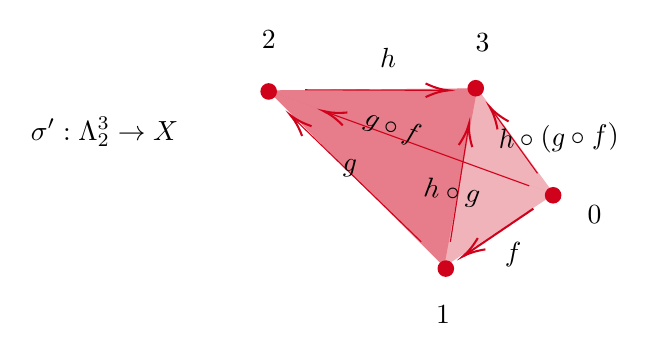
\begin{tikzpicture}[x=0.75pt,y=0.75pt,yscale=-1,xscale=1]
%uncomment if require: \path (0,300); %set diagram left start at 0, and has height of 300
%Shape: Boxed Line [id:dp712419722419394] 
\draw [draw opacity=0][fill={rgb, 255:red, 208; green, 2; blue, 27 }  ,fill opacity=0.3 ]   (277.11,135.11) -- (378.11,134.11) -- (415.11,185.11) -- cycle ;
%Shape: Boxed Line [id:dp06884731912188236] 
\draw [draw opacity=0][fill={rgb, 255:red, 208; green, 2; blue, 27 }  ,fill opacity=0.3 ]   (277.11,135.11) -- (362.11,220.11) -- (415.11,185.11) -- cycle ;
%Shape: Free Drawing [id:dp08767868053848638] 
\draw  [color={rgb, 255:red, 208; green, 2; blue, 27 }  ,draw opacity=1 ][line width=6] [line join = round][line cap = round] (277.58,135.63) .. controls (277.58,135.63) and (277.58,135.63) .. (277.58,135.63) ;
%Shape: Free Drawing [id:dp6329653420526828] 
\draw  [color={rgb, 255:red, 208; green, 2; blue, 27 }  ,draw opacity=1 ][line width=6] [line join = round][line cap = round] (362.92,220.97) .. controls (362.92,220.97) and (362.92,220.97) .. (362.92,220.97) ;
%Shape: Free Drawing [id:dp6342498607996421] 
\draw  [color={rgb, 255:red, 208; green, 2; blue, 27 }  ,draw opacity=1 ][line width=6] [line join = round][line cap = round] (414.62,185.65) .. controls (414.62,185.65) and (414.62,185.65) .. (414.62,185.65) ;
%Straight Lines [id:da526633051382492] 
\draw [color={rgb, 255:red, 208; green, 2; blue, 27 }  ,draw opacity=1 ]   (351.11,208.11) -- (289.55,148.5) ;
\draw [shift={(288.11,147.11)}, rotate = 44.08] [color={rgb, 255:red, 208; green, 2; blue, 27 }  ,draw opacity=1 ][line width=0.75]    (10.93,-3.29) .. controls (6.95,-1.4) and (3.31,-0.3) .. (0,0) .. controls (3.31,0.3) and (6.95,1.4) .. (10.93,3.29)   ;
%Shape: Free Drawing [id:dp44772844349269714] 
\draw  [color={rgb, 255:red, 208; green, 2; blue, 27 }  ,draw opacity=1 ][line width=6] [line join = round][line cap = round] (377.34,134.07) .. controls (377.34,134.07) and (377.34,134.07) .. (377.34,134.07) ;
%Straight Lines [id:da9429587691776815] 
\draw [color={rgb, 255:red, 208; green, 2; blue, 27 }  ,draw opacity=1 ][line width=0.75]    (405.11,192.11) -- (372.77,213.99) ;
\draw [shift={(371.11,215.11)}, rotate = 325.92] [color={rgb, 255:red, 208; green, 2; blue, 27 }  ,draw opacity=1 ][line width=0.75]    (10.93,-3.29) .. controls (6.95,-1.4) and (3.31,-0.3) .. (0,0) .. controls (3.31,0.3) and (6.95,1.4) .. (10.93,3.29)   ;
%Straight Lines [id:da7210386732599512] 
\draw [color={rgb, 255:red, 208; green, 2; blue, 27 }  ,draw opacity=1 ]   (295.1,134.83) -- (362.11,135.1) ;
\draw [shift={(364.11,135.11)}, rotate = 180.23] [color={rgb, 255:red, 208; green, 2; blue, 27 }  ,draw opacity=1 ][line width=0.75]    (10.93,-3.29) .. controls (6.95,-1.4) and (3.31,-0.3) .. (0,0) .. controls (3.31,0.3) and (6.95,1.4) .. (10.93,3.29)   ;
%Straight Lines [id:da9610602919544413] 
\draw [color={rgb, 255:red, 208; green, 2; blue, 27 }  ,draw opacity=1 ]   (365.11,208.11) -- (373.8,153.09) ;
\draw [shift={(374.11,151.11)}, rotate = 98.97] [color={rgb, 255:red, 208; green, 2; blue, 27 }  ,draw opacity=1 ][line width=0.75]    (10.93,-3.29) .. controls (6.95,-1.4) and (3.31,-0.3) .. (0,0) .. controls (3.31,0.3) and (6.95,1.4) .. (10.93,3.29)   ;
%Straight Lines [id:da8120815388496025] 
\draw [color={rgb, 255:red, 208; green, 2; blue, 27 }  ,draw opacity=1 ]   (403.11,181.11) -- (305.99,145.79) ;
\draw [shift={(304.11,145.11)}, rotate = 19.98] [color={rgb, 255:red, 208; green, 2; blue, 27 }  ,draw opacity=1 ][line width=0.75]    (10.93,-3.29) .. controls (6.95,-1.4) and (3.31,-0.3) .. (0,0) .. controls (3.31,0.3) and (6.95,1.4) .. (10.93,3.29)   ;
%Straight Lines [id:da274468734769862] 
\draw [color={rgb, 255:red, 208; green, 2; blue, 27 }  ,draw opacity=1 ]   (407.11,175.11) -- (385.28,144.74) ;
\draw [shift={(384.11,143.11)}, rotate = 54.29] [color={rgb, 255:red, 208; green, 2; blue, 27 }  ,draw opacity=1 ][line width=0.75]    (10.93,-3.29) .. controls (6.95,-1.4) and (3.31,-0.3) .. (0,0) .. controls (3.31,0.3) and (6.95,1.4) .. (10.93,3.29)   ;
%Shape: Boxed Line [id:dp5693420491484811] 
\draw [draw opacity=0][fill={rgb, 255:red, 208; green, 2; blue, 27 }  ,fill opacity=0.3 ]   (277.11,135.11) -- (378.11,134.11) -- (362.11,220.11) -- cycle ;
% Text Node
\draw (161.73,146.92) node [anchor=north west][inner sep=0.75pt]    {$\sigma ':\Lambda _{2}^{3}\rightarrow X$};
% Text Node
\draw (357,237.4) node [anchor=north west][inner sep=0.75pt]    {$1$};
% Text Node
\draw (273.02,105.17) node [anchor=north west][inner sep=0.75pt]    {$2$};
% Text Node
\draw (430,189.4) node [anchor=north west][inner sep=0.75pt]    {$0$};
% Text Node
\draw (376,106.4) node [anchor=north west][inner sep=0.75pt]    {$3$};
% Text Node
\draw (390.11,207.01) node [anchor=north west][inner sep=0.75pt]    {$f$};
% Text Node
\draw (312,167.4) node [anchor=north west][inner sep=0.75pt]    {$g$};
% Text Node
\draw (325.43,141.38) node [anchor=north west][inner sep=0.75pt]  [rotate=-19.28]  {$g\circ f$};
% Text Node
\draw (330,113.4) node [anchor=north west][inner sep=0.75pt]    {$h$};
% Text Node
\draw (351.95,175.66) node [anchor=north west][inner sep=0.75pt]  [rotate=-6.42]  {$h\circ g$};
% Text Node
\draw (386.69,151.9) node [anchor=north west][inner sep=0.75pt]  [rotate=-357.41]  {$h\circ ( g\circ f)$};
        \end{tikzpicture}\]
        它有唯一的延拓
        \[\begin{tikzcd}
	& 1 \\
	0 && 3
	\arrow["{h\circ g}", from=1-2, to=2-3]
	\arrow["f", from=2-1, to=1-2]
	\arrow["{(h\circ g)\circ f}"', from=2-1, to=2-3]
        \end{tikzcd}\]
        依照如上构造,上述$2$-单形确定了$f$与$h\circ g$的合成,即$(h\circ g) \circ f= h\circ (g\circ f)$(即图中$0 \to 3$的两种合成是一致的).\\
        
        综上, $\mathcal{C}$是范畴有典范态射$X\to \nerve\mathcal{C}$,方式为给定$\Delta^n \to X$沿着各个$\Delta^1\xrightarrow{\{j,j+1\}}\Delta^n$拉回以得到态射链.由构造显然有$X_n \to \nerve \mathcal{C}_n$在$n = 0,1$时是双射.在$n \geq 2$时,取$0<i<n$并考虑图表
        \[\begin{tikzcd}
	{\Hom(\Delta^n,X)} & {\Hom(\Delta^n,\nerve \mathcal{C})} \\
	{\Hom(\Lambda_i^n,X)} & {\Hom(\Lambda_i^n,\nerve\mathcal{C})}
	\arrow[from=1-1, to=1-2]
	\arrow["{\text{双射}}"', from=1-1, to=2-1]
	\arrow["{\text{双射}}", from=1-2, to=2-2]
	\arrow[from=2-1, to=2-2]
    \end{tikzcd},\]
    由命题\ref{Pro:边界与尖角图表}可知$\Lambda_i^n$可表为一族$\Delta^{n-1}$和$\Delta^{n-2}$的$\Coker$.由$n=0,1$进行递归即可得知第二行为双射,因此图表交换.
    \item[2. $\Rightarrow$ 3.]通过对$n$进行归纳来证明,当$n = 2$时, $I^2 : 0 \to 1 \to 2$即为内尖角$\Lambda_1^2$根据假设自然满足唯一填充性质.接下来假设对于$k<n$的情况均具有填充性质,现在我们需要将脊$I^n\to X$延拓为$\Delta^n \to X$.观察到$I^n \cap \Delta^{[n]\setminus \{n\}}$即为$I^{n-1}$,同理$I^n \cap \Delta^{[n]\setminus\{0\}}$也是脊.因此根据归纳假设,对于$j = 0,n$存在唯一延拓$\Delta^{[n]\setminus\{j\}}\to X$.考虑两个面的交,即为$\Delta^{[n]\setminus\{0,n\}}$,再交上脊即可得到一个更小的脊,根据假设,两个延拓在相交处是相等的.因此得到映射
    \[
    I^n \cup \Delta^{[n]\setminus\{0\}}\cup\Delta^{[n]\setminus\{n\}} = \Delta^{[n]\setminus\{0\}}\cup\Delta^{[n]\setminus\{n\}} \to X
    \]
    且并起来就是$\Delta^n$.断言存在唯一延拓
    \[\Delta^{[n]\setminus\{0\}}\cup\Delta^{[n]\setminus\{n\}}\cup\Delta^{[n]\setminus\{1\}}\]
    为证明断言,先说明$\Delta^{[n]\setminus\{0\}}\cup\Delta^{[n]\setminus\{n\}}$包含$\Delta^{[n]\setminus\{1\}}$的脊:这是因为$2\leq \leq n-1$与$i \to i+1$均在$\Delta^{[n]\setminus\{0\}}$中,而$0 \to 2$在$\Delta^{[n]\setminus\{n\}}$中($n\geq 3$).因此,由脊可以扩充出唯一的$\Delta^{[n]\setminus\{1\}}\to X$,还需要证明它们在相交处
    \[
    (\Delta^{[n]\setminus\{n\}}\cup \Delta^{[n]\setminus\{0\}})\cap \Delta^{[n]\setminus\{1\}} = \Delta^{[n]\setminus\{1,n\}}\cup \Delta^{[n]\setminus\{0,1\}}.
    \]
    是一致的.而在这些单形中,映射实际上都被在它们的脊所决定,因此得知断言成立.进行归纳即可得到存在唯一的映射$\Lambda_{n-1}^n \to X$,而根据条件2.可以得知这个映射唯一延拓到$\Delta^n$上.
    \item[3. $\Rightarrow$ 2.]考虑单纯集间的映射$\beta : \Lambda_i^n \to X$,需要说明它能够唯一地扩张到$\Delta^n$上.在$n = 2$时, $I^2 : 0 \to 1 \to 2$即为内尖角$\Lambda_1^2$根据假设自然满足唯一填充性质.考虑$n \geq 3$时,有嵌入$I^n \hookrightarrow \Lambda_i^n$根据3.可知存在唯一延拓$\alpha :\Delta^n \to X$.再将这个延拓限制到$\Lambda_i^n$,我们只需要证明$\alpha \mid_{\Lambda_i^n} = \beta$.由于$\Lambda_i^n = \bigcup_{j \neq i}\Delta^{[n]\setminus\{j\}}$,因此可以将问题化约到$\Lambda_i^n$的每个面上进行证明.不难看出
    \[
    \alpha\mid_{\Delta^{[n]\setminus\{0\}}} = \beta\mid_{\Delta^{[n]\setminus\{0\}}}
    \]
    由于这个单纯集的脊是脊$I^n$的子集,并且根据定义有$\alpha \mid_{I^n} = \beta\mid_{I^n}$.因此可以推广为
    \[
    \alpha\mid_{\Delta^{[n]\setminus\{n\}}} = \beta\mid_{\Delta^{[n]\setminus\{n\}}}
    \]
    还需要证明的是
    \[
    \alpha\mid_{\Delta^{[n]\setminus\{j\}}} = \beta\mid_{\Delta^{[n]\setminus\{j\}}}
    \]
    根据假设知$j \neq 0,n$. 首先证明$\alpha\mid_{\Delta^{[n]\setminus\{j-1,j+1\}}} = \beta\mid_{\Delta^{[n]\setminus\{j-1,j+1\}}}$,根据2. $\Rightarrow$ 3.的讨论已然得知这些边要么在$\Delta^{[n]\setminus \{0\}}$中要么在$\Delta^{[n]\setminus \{n\}}$中.因此证明完成.
    \end{enumerate}
\end{proof}
\begin{remark}\label{Rk:外尖角可填充为群胚}
    不难发现,若要求条件2.的适用范围扩大到外尖角上,则$\mathcal{C}$是群胚.只需要取$\Lambda_0^2$, $K$为单纯集的脉,给定映射$\Lambda_0^2 \to K$其对应于
    \[\begin{tikzcd}
	& {C_1} \\
	{C_0} && {C_2}
	\arrow[from=1-2, to=2-3]
	\arrow[dashed, from=2-1, to=1-2]
	\arrow[from=2-1, to=2-3]
    \end{tikzcd}\]
    取$C_0 \to C_2 = \identity$, $C_1 \to C_2 = f$则尖角填充性质说明$f$可逆.
\end{remark}

记$\cate{Cat}$是所有小范畴构成的范畴,态射取为函子.任意函子$F : \mathcal{C} \to \mathcal{C}'$都诱导$\cate{sSet}$中的态射$\nerve F : \nerve \mathcal{C} \to \nerve \mathcal{C}' , (f_1,\cdots,f_n) \to (Ff_1,\cdots,Ff_n)$,由此定义出脉函子$\nerve : \cate{Cat} \to \cate{sSet}$.
\begin{corollary}
    脉函子是全忠实的.
\end{corollary}
\begin{proof}
    根据命题\ref{Pro:脉的刻画}可知$\nerve \mathcal{C} \to \nerve \mathcal{C}'$自然诱导$\mathcal{C}\to \mathcal{C}'$.不难发现与$\nerve$诱导的态射互逆,因此为态射集间的双射,即全忠实.
\end{proof}
\section{Dold-Kan 对应}\label{Dold-Kan 对应}
\begin{wenxintishi}
    本文讲述单纯集上的 Dold-Kan 对应,而 $\infty$-范畴上的版本将在后文讲述.
\end{wenxintishi}
\subsection{Dold-Kan}
令$\mathcal{A}$为加性小范畴,从$\mathcal{A}$出发可以定义单形对象范畴$\mathsf{s}\mathcal{A}$以及链复形范畴$\Chain(\mathcal{A})$.本节主要考虑的是其子范畴$\Chain_{\geq 0}(\mathcal{A})$(见约定\ref{约定:链复形范畴})本节的目的是明确这两个范畴之间的关系,或者精确一点的说,我们将定义三个函子
\[\begin{tikzcd}
	{\Chain_{\geq 0}(\mathcal{A})} & {\mathsf{s}\mathcal{A}}
	\arrow["\DK"{description}, from=1-1, to=1-2]
	\arrow["\chain_*"{description}, curve={height=18pt}, from=1-2, to=1-1]
	\arrow["\normal_*"{description}, curve={height=-18pt}, from=1-2, to=1-1]
\end{tikzcd}\]
接下来我们进行一番婚丧嫁娶将这三个函子的定义叙述
\begin{definition}[非正规化链复形]
    对于$\mathcal{A}$中的半单纯形对象$X$和每个$n\in \Z_{\geq 1}$,定义
    \[
    \partial_n := \sum_{i =0}^n (-1)^i d_i :X_n \to X_{n-1};
    \]
    这使得$(X_n)_{n\geq 0}$连同$(\partial_n)_n$构成$\Chain(\mathcal{A})$中的对象,称为$X$所给出的非正规化链复形或 Moore 链复形,记为 $\chain_*(X)$;因此$\chain_n(X) = X_n$.
\end{definition}
在代数拓扑中我们已经知道$n >1$时$\partial_{n-1} \partial_n = 0$;当然我们可以再重新提一遍,由注记\ref{注记:面态射与退化态射}可知$i<j \Rightarrow d_id_j = d_{j-1}d_i$这也说明
\begin{align*}
    \partial_{n-1}\partial_n = \sum_{i=0}^{n-1}\sum_{j=0}^n (-1)^{i+j}&d_id_j\\
    &= \sum_{0\leq i<j \leq n}(-1)^{i+j}d_{j-1}d_i + \sum_{n-1 \geq i \geq j \geq 0}(-1)^{i+j}d_id_j = 0.
\end{align*}
此构造对于$X$是典范的,这给出函子$\chain_*$.
\begin{definition}[Dold-Kan 构造]
    取定$\Chain_{\geq 0}(\mathcal{A})$中的对象$(A_n,\partial_n)_{n\geq 0}$.依照如下方式定义$\mathsf{s}\mathcal{A}$中对象$\DK(A)$.
    \[
    \DK_n(A) := \bigoplus_{t: [n] \twoheadrightarrow [k]}A_k.
    \]
    对于$\Delta$的任意态射$f: [m] \to [n]$,对应的$f^*: \DK_n (A) \to \DK_m (A)$相对于上述直和分解表为以下矩阵
    \[
    (\Phi_{u,t}:A_k \to A_l)_{\substack{u:[m]\twoheadrightarrow[l]\\t:[n]\twoheadrightarrow[k]}},
    \]
    按照以下方式确定:给定$t :[n] \twoheadrightarrow [k]$,做$tf$的满-单分解
    \begin{equation}\label{公式:满单分解}
    \tag{满-单分解}
        \begin{tikzcd}
	& {[n]} \\
	{[m]} && {[k]} \\
	& {[l]}
	\arrow["t", two heads, from=1-2, to=2-3]
	\arrow["f", from=2-1, to=1-2]
	\arrow["u"', two heads, from=2-1, to=3-2]
	\arrow["v"', hook, from=3-2, to=2-3]
        \end{tikzcd}
    \end{equation}
    \begin{itemize}
        \item 若$l = k$,命$\Phi_{u,t} = \identity$;
        \item 若$l = k-1$,而$v = \delta^0$(遗漏$0$的保序单射),命$\Phi_{u,t} = \partial_k : A_k \to A_{k-1}$;
        \item 其余情形命$\Phi_{u,t}=0$.
    \end{itemize}
    注意到当$f$与$t$给定时,至多存在唯一的$u$使得$\Phi_{u,t} \neq 0$.称其为 Dold-Kan 构造.
\end{definition}
可以验证$\DK A\in \Obj (\mathsf{s}\mathcal{A})$,核心是$(\DK \mathcal{A})_n$的直和项$A_n$和它们在保序单态射下的行为,其它低次直和项$A_k$皆来自满态射$[n]\twoheadrightarrow [k]$诱导的退化,一般情况下$f^*$的定义不过是体现此思路.\\
以上构造是典范的,给出函子$\DK : \Chain_{\geq 0}(\mathcal{A}) \to \mathsf{s} \mathcal{A}$.
\begin{definition}[正规化链复形]
    设$\mathcal{A}$是 Abel 范畴.对$\mathcal{A}$中的半单纯形对象$X$和所有$n\in \Z_{\geq 0}$和$0 \leq k \leq n$定义
    \begin{align*}
        \normal_n(X)&:= \bigcap_{i=1}^n \ker[d_i : X_n \to X_{n-1}], &n \geq 1,\\
        \normal_0(X)&:= X_0.&
    \end{align*}
    连同$X_n \xrightarrow{d_0}X_{n-1}$所诱导的态射族$\normal_n (X) \to \normal_{n-1}(X)$.合理地记为$\partial_n$,它们构成$\Chain_{\geq 0}(\mathcal{A})$中的对象$\normal_*(X)$,称为$X$的正规化链复形.
\end{definition}
\begin{proposition}\label{命题:自然嵌入u_n}
    对如上定义的$X$和每个$n \geq 0$,记$u_n :\normal_n(X) \hookrightarrow X_n$为自然嵌入,则$(u_n)_{n \geq 0}$构成$\Chain_{\geq 0}(\mathcal{A})$中的单态射$u : \normal_*(X) \to \chain_*(X)$,它对$X$满足函子性.
\end{proposition}
\begin{proof}
    直接来自于$\normal_*$和$\chain_*$的定义.
\end{proof}
而后对于 Dold-Kan 定理进行一些必要的铺垫.
\begin{lemma}\label{引理:NDK(A)}
    设$\mathcal{A}$是 Abel 范畴,则对所有的$A\in \Obj(\Chain_{\geq 0}(\mathcal{A})$和$n \geq 0$有$\normal_n \DK(A) = A_n$.这给出函子的同构$\eta : \identity_{\Chain_{\geq 0}(\mathcal{A})} \rightiso \normal_* \DK$.
\end{lemma}
\begin{proof}
    给定$t:[n] \twoheadrightarrow [k]$,注意到当$k<n$时,总可以取$1\leq i \leq n$使得$t^{-1}(t(i))$至少有两个元素,从而$t\delta^i$满,使下图交换
    \[\begin{tikzcd}
	& {[n]} \\
	{[n-1]} && {[k]} \\
	& {[k]}
	\arrow["t", two heads, from=1-2, to=2-3]
	\arrow["{\delta^i}", from=2-1, to=1-2]
	\arrow["{t\delta^i}"', two heads, from=2-1, to=3-2]
	\arrow["\identity"', from=3-2, to=2-3]
    \end{tikzcd}\]
    由此可知$\normal_n \DK(\mathcal{A})$包含于$\identity:[n]\to [n]$对应的直和项$A_n$.然而易证该定义进一步蕴涵$\normal_n \DK(A) = A_n$.而且$\normal_{n+1}\DK(A) \to \normal_n\DK(A)$正是$\partial_{n+1}:A_{n+1}\to A_n$.
\end{proof}
\begin{lemma}\label{引理:DK与N_*伴随}
    设$\mathcal{A}$为 Abel 范畴,先前定义的函子给出伴随对
    \[
    \DK : \Chain_{\geq 0}(\mathcal{A}) \leftrightarrows \mathsf{s} \mathcal{A} : \normal_*
    \]
    \begin{itemize}
        \item 对应的单位态射为引理\ref{引理:NDK(A)}中的$\eta$;
        \item 余单位态射$\varepsilon : \DK \normal_* \to \identity_{\mathsf{s}\mathcal{A}}$描述如下:给定$t : [n] \twoheadrightarrow [k]$,在$\DK \normal_n(X)$中相应的直和项$\normal_k(X)$上,$\varepsilon_{X,n}$是$\normal_k(X) \subset X_k \xrightarrow{t^*}X_n$.
    \end{itemize}
\end{lemma}
\begin{proof}
    给定$A\in \Obj(\Chain_{\geq 0}(\mathcal{A}))$和$X\in \Obj(\mathsf{s}\mathcal{A})$,首要目标是证明
    \[
    \Hom_{\mathsf{s}\mathcal{A}}(\DK(A),X) \xrightarrow{\normal} \Hom_{\Chain_{\geq 0}(\mathcal{A})}(\normal_*\DK(A),\normal_*(X)) \xrightarrow{\eta_A^*}\Hom_{\Chain_{\geq 0}(\mathcal{A})}(A,\normal_*(X))
    \]
    合成为双射.其逆的具体定义如下.给定$\phi = (\phi_n)_{n \geq 0}: A \to \normal_*(X)$,定义态射
    \[
    \Phi_m: (\DK A)_n = \bigoplus_{t: [n] \twoheadrightarrow [k]}A_k \to X_n
    \]
    使得它在对应$t: [n] \twoheadrightarrow [k]$的直和项上是
    \[
    A_k \xrightarrow{\phi_k}\normal_k(X) \subset X_k \xrightarrow{t^*}X_n
    \]
    的合成.对于如上的$t$和任意$f : [m] \to [n]$可做$f$的满-单分解(\ref{公式:满单分解}),并考虑$\mathcal{A}$中的图表
    \[\begin{tikzcd}
	{A_k} & {\normal_k(X)} & {X_k} & {X_n} \\
	{A_l} & {\normal_l(X)} & {X_l} & {X_m}
	\arrow["{\phi_k}", from=1-1, to=1-2]
	\arrow["{\Phi_{u,t}}"', from=1-1, to=2-1]
	\arrow[hook, from=1-2, to=1-3]
	\arrow["{v^*\mid_{\normal_k(X)}}", from=1-2, to=2-2]
	\arrow["{t^*}", from=1-3, to=1-4]
	\arrow["{v^*}", from=1-3, to=2-3]
	\arrow["{f^*}", from=1-4, to=2-4]
	\arrow["{\phi_l}"', from=2-1, to=2-2]
	\arrow[hook, from=2-2, to=2-3]
	\arrow["{u^*}"', from=2-3, to=2-4]
    \end{tikzcd}\]
    左侧方块由$\normal_*(X)$定义可知交换性,中间方块的交换性是显然的,右侧由$tf = vu$所确定.取$\phi \mapsto \Phi$中取$\phi = \identity_{\normal_*(X)}$即可得到余单位态射.
\end{proof}
\begin{lemma}\label{引理:DK在 Ab 上为 伴随等价}
    取$\mathcal{A} = \cate{Ab}$,则$\DK$为等价;或者说$\DK : \Chain_{\geq 0}(\cate{Ab}) \leftrightarrows \cate{sAb}: \normal$为伴随等价.
\end{lemma}
\begin{proof}
    由\parencite[定理 2.6.12.]{李文威卷一}可知,只需要说明余单位态射$\varepsilon$是同构即可.给定$X\in \Obj(\mathsf{s}\mathcal{A})$,我们来验证$\varepsilon_{X,n}: \DK(\normal_*(X))_n \to X_n$对于每个$n \geq 0$即单又满.
    \begin{enumerate}
        \item[单性] 设$x = (x_t)_t \in \DK(\normal_*(X))_n$,其中$t$遍历保序满射$[n] \twoheadrightarrow [k]$.给定$t$,定义保序单射
        \begin{align*}
        s = s_t :[k] &\hookrightarrow [n]\\
         i &\mapsto \min t^{-1}(i)
        \end{align*}
        它满足$ts = \identity_{[k]}$.现在假定$x \neq 0$,记
        \[
        S := \{t : x_t \neq 0\}\neq \varnothing
        \]
        取最小的$k$使得存在属于$S$的$t : [m] \twoheadrightarrow [k]$,再取如此的$t$使得$\sum_{i=0}^k \min t^{-1}(i)$尽可能小,并构造$s$.现在证明$s^*(\varepsilon_{X,n}(x)) = x_t \in X_k$,以此说明$\varepsilon_{X,n}(x) \neq 0$.\\
        基于$\varepsilon_{X,n}$的具体描述,仅需对$t':[n] \twoheadrightarrow [k']$证明$s^*(t')^*(x_{t'}) \neq 0$蕴含$t = t'$即可.命$u := t' s: [k] \to [k']$.当$t' \notin S$时$x_{t'} =0$,故假设$t' \in S$满足$s^*(t')^*(x_{t'}) = u^*(x_{t'}) \neq 0$.\\
        由于$t$保序且为满射,因此$\min t^{-1}(0) =0$,对$t'$亦然,故$u(0) = 0$.又由$x_{t'}\in \normal_{k'} (X)$可推知仅当$\Image(u) \supset \{1,\cdots,k'\}$时才能有$u^*(x_{t'}) \neq 0$.故假设$u$为满, $k$的取法自然蕴含$k'= k$而$u = \identity$.\\
        从而得出$t'(\min t^{-1}(i)) = i$对于$i =  0,\cdots, k$成立,故$\min (t')^{-1}(i) \leq \min t^{-1}(i)$.回顾$t$的取法可知$\min (t')^{-1}(i) = \min t^{-1}(i)$,即$t = t'$.从而$\varepsilon_{X,n}$单.
        \item[满性]通过对$n$递归地证明$\varepsilon_{X,n}$满.兹断言对所有$0 \leq i \leq n$都有
        \[
        \Image(\varepsilon_{X,n})\supset X(i)_n := \bigcap_{i < j \leq n}\ker(d_j) \subset X_n
        \]
        当$i = 0$时 $X(i)_n = \normal_n(X)$,上式容易从$\varepsilon_{X,n}$的具体描述中导出,而我们的目标为$i = n$的情况.现设$n\geq i \geq 1$而$y\in X(i)_n$.关于$n-1$的递归假设和$\varepsilon_{X,n}$蕴含
        \[
        s_{i-1}d_i(y) \in s_{i-1}(\Image(\varepsilon_{X,n-1})) \subset \Image(\varepsilon_{X,n}).
        \]
        另一方面,由于$d_is_{i-1}d_i = d_i d_{i}s_{i} = d_i$以及$j >i$时,$d_j s_{i-1} d_i = s_{i-1} d_{j-1} d_i = s_{i-1} d_i d_j$.因此$y - s_{i-1}d_i (y) \in X(i-1)_n$,由关于$i-1$的递归假设可知其属于$\Image(\varepsilon_{X,n})$.综上$y\in \Image(\varepsilon_{X,n})$.明所欲证.
    \end{enumerate}
\end{proof}
回忆到在 Abel 范畴中我们曾定义幂等元$e\in \End(\mathcal{A})$为满足$e\circ e = e^2 = e$的态射,并且所有幂等元均有核的具有零对象的 $\dcate{Ab}$范畴称为 Karoubi 范畴,接下来介绍本节的核心定理.
\begin{theorem}[A. Dold, D. Kan]
    对于任意加性范畴$\mathcal{A}$,函子$\DK : \Chain_{\geq 0}(\mathcal{A}) \to \mathsf{s} \mathcal{A}$是全忠实的.
    \begin{enumerate}
        \item 若$\mathcal{A}$还是 Karoubi 范畴,则$\DK$为范畴等价.
        \item 若$\mathcal{A}$为 Abel 范畴,则 $\normal_*$ 为 $\DK$ 的拟逆函子$\DK : \Chain_{\geq 0}(\mathcal{A}) \leftrightarrows \mathsf{s} \mathcal{A} : \normal_*$为伴随等价,伴随对的单位和余单位态射由引理\ref{引理:DK与N_*伴随}给出.
    \end{enumerate}
\end{theorem}
\begin{proof}
    考虑函子
    \begin{align*}
    \tilde{h}_{\cal{A}}: \cal{A} &\to \tilde{\cal{A}}^{\land} := \cate{Ab}^{(\cal{A})^{\opposite}}\\
    Y &\mapsto \Hom_{\cal{A}}(-,Y)
    \end{align*}
    它与忘却函子的合成等于Yoneda嵌入$h_{\cal{A}} : \cal{A} \to \cal{A}^{\land}$.函子$\tilde{h}_{\cal{A}}$是全忠实的,这点不过是 $\cate{Ab}$-版本的Yoneda 引理,可以从原版推导:对于任意$Y_1 ,Y_2 \in \Obj(\cal{A})$,合成映射
    \[
    \Hom_{\cal{A}}(Y_1,Y_2) \to \Hom_{\tilde\cal{A}^{\land}}\left(\tilde{h}_{\cal{A}}(Y_1),\tilde{h}_{\cal{A}}(Y_2)\right)\to \Hom_{\cal{A}^{\land}}\left(h_{\cal{A}}(Y_1),h_{\cal{A}}(Y_2)\right)
    \]
    不难发现复合即为双射,而右侧箭头显然单,因此为双射.接下来回归正题.由于$\tilde{A}^{\land}= \cate{Ab}^{(\cal{A})^{\opposite}}$,因此由 $\cate{Ab}$为 Abel 范畴可知$\cate{Ab}^{(\cal{A})^{\opposite}}$为 Abel 范畴.以相同的符号标记$\tilde{h}_{\cal{A}}$在链复形和单纯形对象上诱导的函子,考虑图表
    \[\begin{tikzcd}
	{\Chain_{\geq 0}(\cal{A})} & {\mathsf{s}\cal{A}} \\
	{\Chain_{\geq 0}(\tilde{\cal{A}}^{\land})} & {\mathsf{s}\tilde{\cal{A}}^{\land}}
	\arrow["\DK", from=1-1, to=1-2]
	\arrow["{\tilde{h}_{\cal{A}}}"', from=1-1, to=2-1]
	\arrow["{\tilde{h}_{\cal{A}}}", from=1-2, to=2-2]
	\arrow["\DK"', from=2-1, to=2-2]
    \end{tikzcd}\]
    此图精确到典范同构是交换的.上一段的观察说明两个垂直箭头全忠实,而逐对象地使用关于$\cate{Ab}$的引理\ref{引理:DK在 Ab 上为 伴随等价},可见第二行也为范畴等价,于是第一行$\DK$为全忠实.\\

    对于任意函子$F: \cal{C} \to \cal{C}'$,我们称$X'\in \Obj(\cal{C}')$属于$F$的本质像,如果存在$X\in \Obj(\cal{C})$使得$X'\simeq FX$.搭配引理\ref{引理:DK在 Ab 上为 伴随等价}对于$\Chain_{\geq 0} \to \cate{sAb}$的拟逆的描述,便可以得到以下结论:$X\in \Obj(\cate{s}\cal{A})$属于$\DK$的本质像当且仅当$\normal_n\tilde{h}_{\cal{A}}(X)$对每个$n \geq 0$皆属于$\tilde{h}_{\cal{A}}: \cal{A} \to \tilde{\cal{A}}^{\land}$的本质像.\\
    注意到$\tilde{h}_{\cal{A}}: \cal{A} \to \tilde{\cal{A}}^{\land}$保持有限直和.当$\cal{A}$为 Karoubi 范畴时, $\cal{A} \to \tilde{\cal{A}}^{\land}$的本质像因而对萃取直和项保持封闭;既然$\normal_n\tilde{h}_{\cal{A}}(X)$是$\DK\normal_n\tilde{h}_{\cal{A}}(X)\simeq h_{\cal{A}}(X)_n$的直和项,此时$\DK$全忠实本质满,从而为等价.\\
    最后使用\parencite[定理 2.6.12]{李文威卷一}的伴随等价定理,其确保$\DK$的拟逆总是能扩充为右伴随.当$\cal{A}$为 Abel 范畴时,引理\ref{引理:DK与N_*伴随}已然说明$\normal$为$\DK$的右伴随,从而为拟逆.
\end{proof}
\begin{notation}
    基于此,当$\cal{A}$为 Karoubi 范畴时,可以选定$\DK : \Chain_{\geq 0}(\cal{A}) \to \sf{s}\cal{A}$的拟逆函子,记为$\normal_*$.
\end{notation}
虽然$\normal_*(X)$的初始定义为$\chain(X)$的子对象,但是将其理解为商是更为方便的.以下来说明这一点.\\
考虑 Karoubi 范畴$\cal{A}$以及$X\in \Obj(\sf{s}\cal{A})$对所有$n \geq 0$定义$\cal{A}$中态射$\Psi_n$,其刻画是使得下图对所有$0 \leq j <n$交换
\[\begin{tikzcd}
	{\bigoplus_{0\leq i <n}X_{n-1}} & {X_n} \\
	{X_j}
	\arrow["{\Psi_n}", from=1-1, to=1-2]
	\arrow["{\text{直和项}}", hook, from=2-1, to=1-1]
	\arrow["{s_j}"', from=2-1, to=1-2]
\end{tikzcd}\]
因此考虑$\Coker(\Psi_n)$相当于从$X$中抹去退化部分,至少在$\cal{A}$为 Abel 范畴时可以这么想;次一则结果将说明$\Coker(\Psi_n)$不仅存在还可以通过命题\ref{命题:自然嵌入u_n}中描绘的自然嵌入$u : \normal_*(X) \to \chain_*(X)$来等同于$\normal_n(X)$,这提供了看待$\normal_*(X)$的另一视角.
\begin{proposition}
    上述情境中, $\Coker(\Psi_n)$存在并且典范同构于$\normal_n(X)$,考虑相应的合成$v_n : X_n \twoheadrightarrow \Coker(\Psi_n) \rightiso \normal_n(X)$,则$(v_n)_n$给出态射$v : \chain_*(X) \to \normal_*(X)$它对于$X$具有函子性,并且对于自然嵌入$u : \normal_*(X) \to \chain_*(X)$有$vu = \identity_{\normal_*(X)}$.
\end{proposition}
\subsection{同调计算}
\section{Eilenberg-Zilber定理}\label{Eilenberg-Zilber定理}
\section{统联,锥,映射锥}
本节讲述单纯集的锥这一概念,这一概念实际上牵扯到后文中关于态射空间的很多构造,也与同调代数中映射锥的概念是相关的.\\
记$\cate{FinLin}_{+}$为从有限全序集范畴$\cate{FinLin}$去掉空集所构成的全子范畴,不难发现$\Delta$为其一副骨架,单纯形集可以理解为$\cate{FinLin}_+^{\opposite} \to \cate{Set}$.
%\begin{convention}
%    设$J\in \cate{FinLin}_+$为对象.任意子集$I \subset J$自动为有限全序集;若还有
%    \[
%    \forall  (i,j) \in I \times J, j\leq i \Rightarrow j\in I
%    \]
%    则称$I$为$J$的一个前段,记为$I \sqsubset J$.
%\end{convention}
我们先给出范畴中统联的定义
\begin{definition}
    对于范畴$\mathcal{C}$, $\mathcal{C}'$,定义其统联$\mathcal{C} \star \mathcal{C}'$如下:
    \begin{itemize}
        \item $\Obj(\mathcal{C} \star \mathcal{C}') := \Obj(\mathcal{C}) \sqcup \Obj(\mathcal{C}')$.
        \item $\Hom$集构造如下
        \[
        \Hom_{\mathcal{C}\star \mathcal{C}'} := \left\{
        \begin{array}{ccc}
             \Hom_{\mathcal{C}}(X,Y),&X,Y\in \Obj(\mathcal{C})  \\
             \Hom_{\mathcal{C}'}(X,Y),& X,Y\in \Obj(\mathcal{C}')  \\
             \text{单点集}\{*\}, & X\in \Obj(\mathcal{C}),Y\in \Obj(\mathcal{C}'),\\
             \varnothing, & X\in \Obj(\mathcal{C}'),Y\in \Obj(\mathcal{C}),
        \end{array}{ccc}
        \right.
        \]
    \end{itemize}
\end{definition}
$\mathcal{C}\star \mathcal{C}'$以自明的方式构成范畴,不难发现统联不是对称的.为定义出单纯集上的统联,我们需要引入分划这一概念
\begin{definition}[分划]
    给定全序集$J$,定义$\cate{Cut}(J)$为
\end{definition}
\section{本讲习题}
        \chapter{$\infty$-范畴}
为了说明一个$\infty$-范畴$\mathcal{C}$应当是什么样的,不妨考虑两个极端的情况.若$\mathcal{C}$中的每个态射均可逆,则$\mathcal{C}$等价于一个拓扑空间$X$的基本$\infty$-群胚.此时高阶范畴论约化为经典的同伦论.而若$\mathcal{C}$在$n>1$时没有非平凡$n$-态射,此时$\mathcal{C}$等价于一般的范畴.因此,一般情况应该抓住这二者共同的特征,即我们需要一类表现形式既像范畴又像拓扑空间的对象,而这就是单纯集.

以下为无穷范畴,Kan复形,单纯集,拓扑空间之间的关系.
\[\begin{tikzcd}
	{\{\text{Categories}\}} & {\{\infty\text{-Categories}\}} & {\{\text{Kan Complexes}\}} \\
	& {\cate{sSet}} & {\cate{Top}}
	\arrow["{N_{\bullet}}", hook, from=1-1, to=1-2]
	\arrow["\subset"{marking, allow upside down}, draw=none, from=1-2, to=2-2]
	\arrow["\subset"{marking, allow upside down}, draw=none, from=1-3, to=1-2]
	\arrow["{\Sing_{\bullet}}", from=2-3, to=1-3]
\end{tikzcd}\]
本节来讲述Kan复形以及拟范畴理论,在此之前请回忆在导言中所提到过``我们需要一类表现形式既像范畴又像拓扑空间的对象.''这将在后文描述出拟范畴时起到巨大作用.
\section{Kan 复形与 $\infty$-范畴}
\begin{definition}[Kan复形]
    令$X$为一个单纯集.若所有的尖角均可填充,即对于$0\leq i\leq n$以下图表
    \[\begin{tikzcd}
	{\Lambda_i^n} & X \\
	{\Delta^n}
	\arrow[from=1-1, to=1-2]
	\arrow[hook, from=1-1, to=2-1]
	\arrow[dashed, from=2-1, to=1-2]
    \end{tikzcd}\]
    交换.则称$X$为Kan复形.
\end{definition}
接下来我们展现单纯集的便利性,根据注记\ref{Rk:外尖角可填充为群胚},可知当$X$是Kan复形时,它会作为一个$\infty$-群胚,而当其满足内尖角填充性质时,它可以根据命题\ref{Pro:脉的刻画}来变成一般的范畴.基于这一观察,我们希望可以得到一些更合适的单纯集来作为一般的$\infty$-范畴的模型.\\

首先考虑任意一个单纯集$X$.我们可以尝试着将$X$想象成一个范畴,首先$X$中的点(即$X_0$的元素)就是其对象,态射则为$X$中的边($X_1$中的对象).一个$2$-单形$\sigma : \Delta^2 \to X$应当被视为图表
\[\begin{tikzcd}
	& B \\
	A && C
	\arrow["\psi", from=1-2, to=2-3]
	\arrow["\phi", from=2-1, to=1-2]
	\arrow["\theta"', from=2-1, to=2-3]
\end{tikzcd}\]
以及$\theta$与$\psi \circ \phi$的同伦,这将被视为图表的``交换性''(在高阶范畴论中,交换性不仅仅是一个条件:同伦$\theta \simeq \psi \circ \phi$是额外的资料.)高阶单形可以被认为反映了高阶图表的交换性.\\

坏消息是,对于一般的单纯集$X$,上文的类比就略显乏力.这个问题的本质在于,哪怕我们可以把$X$中的$1$-单形视为态射,但是它们的合成却不总是存在.比如说取$\nerve \mathcal{C}$这个例子,对于态射$\theta : A\to C$,若存在一个$2$-单形$\sigma : \Delta^2 \to X$使得其表现为前文所示的交换图则称$\theta$为态射$\phi : X \to Y$与态射$\psi :Y \to Z$的合成.现在我们需要考虑两个潜在的问题:
\begin{itemize}
    \item 所需的$2$-单形$\sigma$不一定总是存在.
    \item 即使其存在也不一定唯一,即我们可能不止$\theta$一个选择.
\end{itemize}
存在性要求$\sigma$总是可以被表述为单纯集$X$的延拓条件.注意到可组合的态射偶$(\psi ,\phi)$事实上确定了一个单纯集间的映射$\Lambda_1^2 \to X$.因此,断言$\sigma$总是能够被表述为一个延拓条件:任意形如$\Lambda_1^2 \to X$的单纯形间的映射都可以延拓到$\Delta^2$上,归结为以下图表
\[\begin{tikzcd}
	{\Lambda_1^2} & K \\
	{\Delta^2}
	\arrow[from=1-1, to=1-2]
	\arrow[hook, from=1-1, to=2-1]
	\arrow[dashed, from=2-1, to=1-2]
\end{tikzcd}\]
而$\theta$的唯一性又是另一个问题.事实证明要求$\theta$被唯一确定是不必要(并且不自然)的.为了说明这一点,让我们回到例\ref{Exp:群胚}上.对于群胚中的两条道路,若它们同伦则被认为是等价的.基本群胚中,复合是由道路的合成给出的,即给定道路$q,p : [0,1] \to X$使得$p(0) = x$而$p(1)=q(0) = y$,且$q(1) = z$,则$p$与$q$的复合应当为一条连接$x$与$z$的道路.有很多方法得到这样连接$p$与$q$的道路.最简单的方式无非是
\[
r(t) = \left\{\begin{array}{cc}
     p(2t)&\text{若}0\leq t \leq \frac{1}{2}  \\
     q(2t-1)&\text{若}\frac{1}{2}\leq t\leq 1. 
\end{array}\right.
\]
然而,同样可以使用以下方式进行合成
\[
r'(t) = \left\{\begin{array}{cc}
   p(3t)  & \text{若} 0\leq t \leq \frac{1}{3} \\
   q(\frac{3t-1}{2})& \text{若} \frac{1}{3}\leq t\leq 1.
\end{array}\right.
\]
由于$r$与$r'$是同伦的,因此这并不妨碍选取.\\
但是从$2$-范畴的角度上进行考虑时,这个问题就变得复杂了.考虑拓扑空间$E$的基本2-群胚,为使得态射的合成有明确的定义,我们必须选择一个等式来代替全部等式.此外,这并没有一个特别合适的选择.举个例子,前文所述的两个等式都无法表示严格的结合律.\\
这个教训给我们带来了一个启发:在高阶范畴处,我们不应该要求两个态射具有唯一确定的组合(即唯一的填充).在基本群胚的例子中,道路的复合有许多种选择,但是它们是相互同伦的.此外,根据高阶范畴论的哲学原理:任何与复合同伦的道路都应当与复合本身一样好.从这一点出发,我们应当将复合视为一种关系而非函数,这在单纯集的形式中可以很好地得到展现:一个2-单形$\sigma :\Delta^2 \to X$应当被视为$d_0(\sigma) \circ d_2(\sigma)$同伦于$d_1(\sigma)$的``证据''.\\

那么具体是什么样的条件才能够保证一个单纯集$X$表现得像一个更高阶的范畴呢?基于前文的讨论,我们发现这只需要让$X$满足对于尖角$\Lambda_i^n$的填充性质,但是根据注记\ref{Rk:外尖角可填充为群胚}以及命题\ref{Pro:脉的刻画}可知只需要对于内尖角进行填充即可.因此得到定义
\begin{definition}
    $\infty$-范畴是一个满足以下性质的单纯集$X$:对任意的$0<i<n$以及任意单纯集间的映射$\Lambda_i^n \to X$,都可以填充为$f: \Delta^n \to K$.
\end{definition}
\begin{example}
    前文所述的Kan复形以及脉均为$\infty$-范畴的例子.
\end{example}
\section{单纯集的同伦范畴}
\begin{definition}
    $\infty$-范畴$X$与$Y$之间的函子即为相应单纯集之间的映射.换句话说, $\infty$-范畴所构成的范畴实际上是$\cate{sSet}$的全子范畴.
\end{definition}
由前文关于$\infty$-范畴的讨论可以得到以下概念:
\begin{definition}[$1$-单形等价]\label{定义:1-单形等价}
    令$X$为单纯集,称两个从$x$到$y$的$1$-单形$f$和$g$是等价的当且仅当存在一个$2$-单形$\sigma : \Delta^2 \to X$使得
    \begin{enumerate}
        \item $\sigma\mid_{\Delta^{\{0,1\}}} = f$.
        \item $\sigma\mid_{\Delta^{\{0,2\}}} = g$.
        \item $\sigma\mid_{\Delta^{\{1,2\}}} = \identity_y$.
    \end{enumerate}
\end{definition}
而后我们研究如何将单纯集对应到一般范畴上.
\begin{definition}[同伦范畴]
    令$X$为单纯集,定义范畴$hX$为以下资料:
    \begin{itemize}
        \item 对象:$X_0$中的元素.
        \item 态射:$X_1$所生成的态射,对于任意1-单形$f:\Delta^1 \to X$,它都被视为从$d_1(f)$到$d_0(f)$的态射.
        \item 复合:态射箭的自由复合记为$f\star g$,商去以下关系
        \begin{enumerate}
            \item 1-单形$s_0(x)$是$x$的恒等态射.
            \item 对于每个$2$-单形$\sigma:\Delta^2 \to X$且边界为三元组$(f,g,h)$,则$h= g\star f$/
            \item 若$f\sim f'$则$f\star g\sim f'\star g$且$g'\star f\sim g'\star f'$.
        \end{enumerate}
    \end{itemize}
    称其为$X$的同伦范畴,同伦范畴中的态射称为同伦类.
\end{definition}

并且同伦范畴与脉有以下伴随关系
\begin{proposition}\label{命题:h与N相伴随}
    具有伴随对$h \dashv \nerve$
    \[
        h: \operatorname{sSet} \leftrightarrows \operatorname{Cat}:\nerve
    \]
    其中$\nerve$为范畴的脉.且有$h(\nerve(\mathcal{C}))\simeq \mathcal{C}$.
\end{proposition}
\begin{proof}\parencite[Proposition 1.2.18]{Land}.其中$h(\nerve(\mathcal{C}))\simeq \mathcal{C}$读者自证不难.\end{proof}
若$X = \mathcal{C}$为无穷范畴,则可通过同伦范畴来描述其内一些箭头的性质.
\section{群胚与极大子$\infty$-群胚}
\begin{definition}[等价]
    $\infty$-范畴$\mathcal{C}$中的态射$f$若其在$h\mathcal{C}$的像为同构,则称其为等价.
\end{definition}
可以通过$2$-单形来描述等价
\begin{proposition}\label{命题:2-单形描述等价}
    $\infty$-范畴$\mathcal{C}$中态射$f: x \to y$为等价当且仅当存在$2$-单形$\sigma^l : \Delta^2 \to \mathcal{C}$以及$\sigma^r : \Delta^2 \to \mathcal{C}$使得
    \[
    \sigma^l\mid_{\Lambda_0^2} = (f,\identity_x), \sigma^r \mid_{\Lambda_{2}^2} = (f,\identity_y)
    \]
\end{proposition}
此处$(g,h)$的对应方式与推论\ref{推论:尖角变体}无异.
\begin{proof}
\begin{enumerate}
    \item[($\Leftarrow$)] 若$2$-单形$\sigma^l$存在,则$\sigma^l\mid_{\Delta^{\{1,2\}}}$即为$f$在$h\mathcal{C}$中的像的左逆.类似地, $\sigma^r\mid_{\Delta^{\{0,1\}}}$为$f$在$h\mathcal{C}$中的像的右逆,因此$f$在$h\mathcal{C}$中像的左右逆均存在,即$f$为等价.
    \item[($\Rightarrow$)] 若$f$为等价,则存在态射$g: y \to x$使其同伦类$[g]$为$[f]$的逆,使得$[gf]$与$[fg]$分别为$h\mathcal{C}$中的$\identity_x$和$\identity_y$.在此处只需要考虑$[g\circ f]$至于$[f\circ g]$可以用来类似地构造$\sigma^r$.不难发现存在$\eta : \sigma^2 \to \mathcal{C}$作为$h$与$g\circ f$同伦的依据,而后由于$[gf] = \identity_x$,因此存在$\hat{\eta}: \sigma_2 \to \mathcal{C}$作为$h$与$\identity_x$同伦的依据,此外还有一个自明的$2$-单形(象征$g$与其自身同伦)因此这$3$个$2$-单形构成内尖角$\Lambda_2^3 \to \mathcal{C}$,展现成图表即为
    \[\begin{tikzcd}
	& x \\
	x && y \\
	&& x
	\arrow["{\identity_x}", from=2-1, to=1-2]
	\arrow["f", from=2-1, to=2-3]
	\arrow["h"', from=2-1, to=3-3]
	\arrow["g"', from=2-3, to=1-2]
	\arrow["g", from=2-3, to=3-3]
	\arrow["{\identity_x}"{description, pos=0.3}, from=3-3, to=1-2]
    \end{tikzcd}\]
    由$\mathcal{C}$为$\infty$-范畴的内尖角填充性质即可得到$\sigma^l$的存在性.
\end{enumerate}
   
\end{proof}
此外,我们可以引入$\infty$-群胚.
\begin{definition}
    设$\mathcal{C}$为$\infty$-范畴,若其内所有态射皆为等价,则称其为$\infty$-群胚.
\end{definition}
我们可以在$\infty$-范畴内部去定义其子$\infty$-群胚.
\begin{definition}[极大子$\infty$-群胚]\label{定义:极大子无穷群胚}
    在一般范畴中极大子群胚由其内所有同构所构成的子范畴,并且记为$\mathcal{C}^{\simeq}\subset \mathcal{C}$.对于$\infty$-范畴$\mathcal{C}$,可以类似定义其极大子$\infty$-群胚为单纯集的拉回
    \[\begin{tikzcd}
	{\mathcal{C}^{\simeq}} & {\mathcal{C}} \\
	{\nerve(h\mathcal{C}^{\simeq})} & {\nerve(h\mathcal{C})}
	\arrow[from=1-1, to=1-2]
	\arrow[from=1-1, to=2-1]
	\arrow[from=1-2, to=2-2]
	\arrow[from=2-1, to=2-2]
    \end{tikzcd}\]
\end{definition}
\begin{remark}
    对于一般范畴$\mathcal{C}$有$\nerve(\mathcal{C})^{\simeq} = \nerve(\mathcal{C}^{\simeq}$这只需要考虑以下交换图
    \[\begin{tikzcd}
	{\nerve(\mathcal{C})^{\simeq }} & {\nerve(\mathcal{C})} \\
	{\nerve(h(\nerve(\mathcal{C}))^{\simeq})} & {\nerve(h(\nerve(\mathcal{C})))} \\
	{\nerve(\mathcal{C}^{\simeq})} & {\nerve(\mathcal{C})}
	\arrow[from=1-1, to=1-2]
	\arrow[from=1-1, to=2-1]
	\arrow[from=1-2, to=2-2]
	\arrow[from=2-1, to=2-2]
	\arrow["\simeq"', from=2-1, to=3-1]
	\arrow["\simeq", from=2-2, to=3-2]
	\arrow[from=3-1, to=3-2]
    \end{tikzcd}\]
    由命题\ref{命题:h与N相伴随}可知同构.
\end{remark}
不难看出$\infty$-范畴中$n$-单形在极大子$\infty$-群胚中当且仅当其所有边均为等价.
\begin{proposition}
    $\infty$-范畴中的极大子$\infty$-群胚确实是一个$\infty$-群胚,并且是$\infty$-范畴所包含的最大$\infty$-群胚.
\end{proposition}
\begin{proof}
    设$\mathcal{C}$为$\infty$-范畴,首先证明$\mathcal{C}^{\simeq}$为一个$\infty$-范畴.这需要证明其满足内尖角填充性质.因此考虑图表
    \[\begin{tikzcd}
	{\Lambda_i^n} & {\mathcal{C}^{\simeq}} & {\mathcal{C}} \\
	{\Delta^n}
	\arrow[from=1-1, to=1-2]
	\arrow[from=1-1, to=2-1]
	\arrow["{\subset }"{marking, allow upside down}, draw=none, from=1-2, to=1-3]
	\arrow[dashed, from=2-1, to=1-2]
    \end{tikzcd}\]
    其中$0<i<n$.由于$\mathcal{C}$为$\infty$-范畴,因此该提升问题在$\mathcal{C}$中必然有解,只需要证明解落在$\mathcal{C}^{\simeq}$中即可,根据$\mathcal{C}^{\simeq}$的定义,这相当于要证明$\Delta^n\to \mathcal{C}$诱导态射
    \[
        \Lambda_i^n \to \Delta^n \to \mathcal{C}\to \nerve(h\mathcal{C})
    \]
    并且其像包含在$\nerve(h\mathcal{C}^{\simeq})$内.回忆到范畴的脉中$n$-单形由其限制在脉的脊上所决定而每一个内尖角都包含脊,从而断言成立.这也说明$\mathcal{C}^{\simeq}$包含$\mathcal{C}$中所有的等价.特别地,可以得到$h(\mathcal{C}^{\simeq}) = (h\mathcal{C})^{\simeq}$,因此$\mathcal{C}^{\simeq}$是$\infty$-范畴,而且蕴含极大性.
\end{proof}
\begin{theorem}[Joyal]
    设$\mathcal{C}$为$\infty$-范畴.则$\mathcal{C}$为Kan复形当且仅当$h\mathcal{C}$为群胚.
\end{theorem}
\begin{proof}
    见\cite{Joyal}.
\end{proof}
\begin{lemma}
    Kan 复形是 $\infty$-群胚.
\end{lemma}
\begin{proof}
    只需要说明 Kan 复形中任意态射均为等价即可,令$X$为 Kan 复形,由 Kan 复形的定义立刻得到对于任意$f \in X$,考虑$(f,\identity_x)$所构成的外尖角$\Lambda_0^2 \to \mathcal{C}$以及$(f,\identity_y)$所构成的外尖角$\Lambda_2^2 \to \mathcal{C}$都具有填充,因此由命题\ref{命题:2-单形描述等价}可知其为等价.
\end{proof}
\begin{fact}\label{事实:群胚}
    群胚不是群的推广而是集合的推广,这是因为群的$1$-范畴不等价于单对象群胚的$2$-范畴.只有在选定基点后,才能够典范的取出群.当然,群胚这一概念比群更加基本,因为其没有代数结构.\\
    在高阶范畴论中, $\infty$-群胚可以视为集合一类的最为基础的结构,因为如绪言所说,它对应于拓扑空间,记录了拓扑空间中所有的同伦信息.\\
    这一事实将会在后文中反复用到.
\end{fact}
本节以一些 Kan 复形的性质以及定义作为结尾.
\begin{definition}[Kan 复形的基本群胚]\label{定义:Kan 复形的基本群胚}
    当$X$为 Kan 复形时,群胚$hX$称为$X$的基本群胚,记为$\pi_{\leq 1}(X)$.
\end{definition}
\begin{example}
    \begin{itemize}
        \item Kan 复形在乘积下稳定.
        \item Kan 复形在余积下稳定,或者说若$S = \bigsqcup_{i\in I}S_i$则$S$为 Kan 复形当且仅当 $S_i$均为 Kan 复形.
    \end{itemize}
\end{example}
\begin{proposition}
    $\cate{sSet}$中的群对象的底单纯集是 Kan 复形.
\end{proposition}
\begin{proof}
    见\parencite[\href{https://kerodon.net/tag/00MG}{00MG}]{Kerodon}.
\end{proof}
\begin{proposition}\label{命题: Kan 复形乘积的连通性}
    若$S = \prod_{i\in I}S_i$为 Kan 复形,则
    \[
        \pi_0(S) \to \prod_{i\in I}\pi_0(S_i)
    \]
    为双射.特别地,$S$是连通的当且仅当$S_i$均连通.
\end{proposition}

\section{本讲习题}
\begin{exercise}
    验证:对于拓扑空间$E$,其对应的奇异单纯集$\Sing(E)$是 Kan 复形.
\end{exercise}
\begin{solution}
    利用几何实现函子,可以将$\sigma_0:\Lambda_i^n \to \Sing(E)$转化为$f_0:|\Lambda_i^n| \to E$.只需要说明$f_0$可以写为分解
    \[
        |\Lambda_i^n| \hookrightarrow |\Delta^n|\xrightarrow{f} E
    \]
    即可.为此,可以利用$\Lambda_i^n$的几何实现与$|\Delta^n|$之间的关联.
\end{solution}
\begin{exercise}[骨架与同构]
    令$f: X \to Y$为诱导出$2$-骨架之间同构$\sk_2(X) \to \sk_2(Y)$的单纯集之间的映射,试证明其诱导的同伦范畴之间的函子$hf : hX\to hY$为等价.
\end{exercise}
\begin{exercise}[填色游戏]
    令$X$为脊可填充(即$I^n \to \Delta^n$满足提升性质)且对于$3$-内尖角具有提升性质,令$f$和$g$为$\mathcal{C}$中可复合的$1$-单形.则
    \begin{enumerate}
        \item 存在$f$与$g$的复合.
        \item 定义\ref{定义:1-单形等价}所提出的``等价''确实是一个等价关系.
        \item 任意两个可复合的态射$f$和$g$在定义\ref{定义:1-单形等价}的意义下是等价的.
        \item 给定$2$-单形$\sigma$,且$\sigma\mid_{\Delta^{\{0,1\}}}=\identity_x$,$\sigma\mid_{\Delta^{\{1,2\}}}=h$,$\sigma\mid_{\Delta^{\{0,2\}}}=h'$,则$h' \sim h$.
    \end{enumerate}
\end{exercise}
\begin{solution}
    1. 是由定义立刻得出的而2.,3.,4.都是填色游戏,比如2.中对称性可以考虑
    \[\begin{tikzcd}
	& y \\
	&& y \\
	x && y
	\arrow["{\identity_y}"', from=2-3, to=1-2]
	\arrow["{\identity_y}", from=2-3, to=3-3]
	\arrow["f", from=3-1, to=1-2]
	\arrow["f", from=3-1, to=2-3]
	\arrow["g"', from=3-1, to=3-3]
	\arrow["{\identity_y}"', from=3-3, to=1-2]
    \end{tikzcd}\]
    利用填充性质进行涂色即可,传递性考虑
    \[\begin{tikzcd}
	& y \\
	&& y \\
	x && y
	\arrow["{\identity_y}"', from=2-3, to=1-2]
	\arrow["{\identity_y}", from=2-3, to=3-3]
	\arrow["h", from=3-1, to=1-2]
	\arrow["f", from=3-1, to=2-3]
	\arrow["g"', from=3-1, to=3-3]
	\arrow["{\identity_y}"', from=3-3, to=1-2]
    \end{tikzcd}\]
    剩下命题请读者自行涂色.
\end{solution}
\begin{exercise}
    范畴的脉是$2$-余骨架.
\end{exercise}
\begin{solution}
    考虑交换图表
    \[\begin{tikzcd}
	{\Fct(hX,\mathcal{C})} & {\Hom_{\cate{sSet}}(X,\nerve\mathcal{C})} \\
	{\Fct(h(\sk_2X),\mathcal{C})} & {\Hom_{\cate{sSet}}(\sk_2X,\nerve\mathcal{C})} & {\Hom_{\cate{sSet}}(X,\cosk_2\nerve\mathcal{C})}
	\arrow[from=1-1, to=1-2]
	\arrow[from=1-1, to=2-1]
	\arrow[from=1-2, to=2-2]
	\arrow[from=1-2, to=2-3]
	\arrow[from=2-1, to=2-2]
	\arrow[from=2-2, to=2-3]
    \end{tikzcd}\]
    利用伴随性以及前文练习验证交换性即可.
\end{solution}
\begin{exercise}
    $\infty$-范畴的乘积以及余积均为$\infty$-范畴.
\end{exercise}
\begin{solution}
    对于乘积的情况,我们可以单独对于每个$\infty$-范畴进行处理,然后延拓到乘积之上.\\
    对于余积的情况,我们注意到$\Lambda_i^n$以及$\Delta^n$都是连通的,因此我们只需要在一个$\infty$-范畴上解决延拓问题即可.
\end{solution}

        \chapter{单纯范畴}
令$\operatorname{Top}$表示拓扑空间范畴.根据定义,$\operatorname{Top}$中态射均为连续函数.在同伦论中,我们并不关心函数自身,而是关心它们之间的同伦:即,连续函数$h:[0,1]\times X\to Y$.更一般地,对于每个$n\geq 0$我们可以考虑
\[
    \Hom_{\operatorname{Top}}(X,Y)_n = \{\text{连续函数}\sigma : |\Delta^n| \times X\to Y\}
\]
此处$|\Delta^n|$为几何实现.集合$\{\Hom_{\operatorname{Top}}(X,Y)_n\}_n$可以被嵌入到单纯集$\Hom_{\operatorname{Top}}(X,Y)_{\bullet}$中,并且$(X,Y)\mapsto \Hom_{\operatorname{Top}}(X,Y)_{\bullet}$赋予$\operatorname{Top}$一个$\Cat_{\operatorname{sSet}}$-充实结构(当然我们后面会简写为$\Cat_{\Delta}$),我们称其为单纯范畴.正如奇异单纯集$\operatorname{Sing}_{\bullet}(X) = \Hom_{\operatorname{Top}}(*,X)_{\bullet}$可以被视为拓扑空间$X$的同伦型的组合编码一般.$\operatorname{Top}$的单纯充实化从同伦论角度对于拓扑空间进行的组合编码.\\
此外, \cite{SixFunctors}里$\Cat_{\infty}$也需要通过单纯范畴及其同伦脉来定义(见\ref{平凡 Kan 纤维化的应用}一节).
\section{单纯范畴定义}
\begin{notation}
    令$\mathcal{V}$为幺半范畴,则$\operatorname{Cat}_{\mathcal{V}}$表示$\mathcal{V}$-充实范畴所构成的范畴,即其对象为$\mathcal{V}$-充实范畴而态射为$\mathcal{V}$-充实函子.
\end{notation}
首先需要一些必要的幺半范畴引理
\begin{lemma}
    若$\Phi : \mathcal{V} \to \mathcal{V}'$为幺半范畴之间的右松幺半函子,则将$\Phi$应用在$\iHom$-对象上即可得到函子$\Phi_* : \operatorname{Cat}_{\mathcal{V}}\to \operatorname{Cat}_{\mathcal{V}'}$.事实上,这种结构定义出
    \[
        \operatorname{MonCat} \to \operatorname{Cat}
    \]
    这样一个从(小)幺半范畴构成的2-范畴(0-态射:幺半范畴,1-态射:右松幺半函子,2-态射:幺半自然变换)到由(小)范畴构成的2-范畴(0-态射:范畴,1-态射:函子,2-态射:自然变换)的2-函子.特别地,$\mathcal{V}$与$\mathcal{V}'$的幺半伴随决定了充实范畴的幺半伴随.
\end{lemma}
\begin{proof}
    见\parencite[Lemma 1.2.37]{Land}.
\end{proof}
通过上述引理,就可以将充实范畴对应回一般的范畴,称为底范畴.
\begin{definition}\label{定义:底范畴}
    令$\mathcal{V}$为幺半范畴,且$\mathcal{C}$为一个$\mathcal{V}$-充实范畴.则其底范畴$u\mathcal{C}$由松幺半函子
    \[
        \Hom(\identity,-):\mathcal{V} \to\operatorname{Set}
    \]
    形式化的写出即为
    \[
        u\mathcal{C} = \Hom_{\mathcal{V}}(\identity,-)_*(\mathcal{C})\in \operatorname{Cat}_{\operatorname{Set}}=\operatorname{Cat}
    \]
\end{definition}
接下来介绍单纯范畴
\begin{definition}[单纯范畴]
    我们把充实于单纯集范畴的范畴称为单纯范畴.此处单纯集范畴$\operatorname{sSet}$通过积结构可以视为幺半范畴.本节将全体单纯范畴所构成的范畴简写为$\operatorname{Cat}_{\Delta}$.
\end{definition}
\begin{example}
    考虑拓扑空间构成的范畴$\cate{Top}$.它可以通过以下方式转变为单纯范畴:给定一对拓扑空间$X$, $Y$.定义单纯集$\iHom_{\cate{Top}}(X,Y)$如下
    \[
    \iHom_{\cate{Top}}(X,Y)_n = \Hom_{\cate{Top}}(|\Delta^n|\times X,Y)
    \]
    特别地,其每个顶点都可以视为从$X$到$Y$的连续函数$f$.此外,不难发现考虑$X$为单点时, $\iHom(*,Y) \simeq \Sing(Y)$.
\end{example}
\begin{remark}
    通常来说单纯范畴指代的是范畴中的一个单形对象,即一个函子$\Delta^{\opposite}\to\operatorname{Cat}$.这似乎与单纯范畴的定义冲突,以下引理将对其进行解释.
\end{remark}


\begin{lemma}
    $\operatorname{Cat}_{\Delta}$可以通过$(\ev_n)_*:\operatorname{Cat}_{\Delta} \to \operatorname{Cat}$得到全忠实嵌入$\operatorname{Cat}_{\Delta} \to \Fct(\Delta^{\opposite},\operatorname{Cat})$.事实上可以得到以下拉回
\[\begin{tikzcd}
	{\Cat_{\Delta}} && {\Fct(\Delta^{\opposite},\Cat)} \\
	{\operatorname{Set}} && {\Fct(\Delta^{\opposite},\operatorname{Set})}
	\arrow["{\mathcal{C}\mapsto ((\ev_n)_*\mathcal{C})_{\bullet}}", from=1-1, to=1-3]
	\arrow["{\operatorname{Ob}}", from=1-1, to=2-1]
	\arrow["{\operatorname{Ob}}"', from=1-3, to=2-3]
	\arrow[from=2-1, to=2-3]
\end{tikzcd}\]
\end{lemma}
可以利用$\operatorname{Cat}$是完备且余完备的来说明$\operatorname{Cat}_{\Delta}$是完备且余完备的.进一步,可以不局限于单纯集范畴,可以推广为任意小范畴$\mathcal{C}$的预层范畴$\mathcal{C}^{\land}$.\\
我们可以验证常值函子与$\pi_0,\ev_0$都是典范幺半的.
\begin{lemma}\label{引理:三个函子均幺半}
    函子$c: \operatorname{Set} \to \operatorname{sSet}$以及$\pi_0,\ev_0:\operatorname{sSet}\to \operatorname{Set}$均为典范幺半的.
\end{lemma}
\begin{proof}
    断言每个函子$F:(\mathcal{V},\times,*) \to (\mathcal{W},\times,*)$都是典范左松幺半的.左松幺半结构态射给定如下
    \begin{enumerate}
        \item $F(*) \to *$,即唯一一个到$\mathcal{W}$的终对象的态射,且
        \item $F(X\times Y) \to F(X) \times F(Y)$,它由$F$作用在两个投影
        \[
            X\leftarrow X\times Y \rightarrow Y
        \]
        所给出.\\
        因此只需要检查我们所给出的函子确实具有左松幺半结构即可,即左松幺半结构所对应的态射在前文的函子中是同构.对于$c$以及$\ev_0$,由定义即知具有左松幺半结构.而$\pi_0$函子需要一些额外的论证.需要检查态射
        \[
            \pi_0(X\times Y) \to \pi_0(X)\times \pi_0(Y)
        \]
        是双射.根据定义可知$\pi_0$作用后的单纯集具有以下交换图表
        \[\begin{tikzcd}
	    {(X\times Y)_0} & {X_0\times Y_0} \\
	    {\pi_0(X\times Y)} & {\pi_0(X)\times \pi_0(Y)}
	    \arrow["\simeq", from=1-1, to=1-2]
	    \arrow[two heads, from=1-1, to=2-1]
	    \arrow[two heads, from=1-2, to=2-2]
	    \arrow[from=2-1, to=2-2]
        \end{tikzcd}\]
        由于顶部水平态射是双射,因此给出左松幺半结构为满射.由于$\pi_0(X\times Y)$中对应关系的生成元可以被提升到$(X\times Y)_0$, $\pi_0(X)$和$\pi_0(Y)$亦是如此,并且$\ev_1$也具有幺半结构,因此得知双射.并且不难验证$\pi_0(*)\to*$是同构.
    \end{enumerate}
\end{proof}
\begin{definition}
    \begin{enumerate}
        \item $c= c_* : \operatorname{Cat} \to \operatorname{Cat}_{\Delta}$,将一个范畴送到常值单纯集填充的充实范畴.
        \item $h = (\pi_0)_*:$,称为单纯范畴的同伦范畴,以及
        \item $u = (\ev_0)_*:\operatorname{Cat}_{\Delta} \to \operatorname{Cat}$,称为底范畴,在不会造成歧义时也直接写作$\mathcal{C}_0$.
    \end{enumerate}
    注意到$\ev_0 = \Hom_{\operatorname{sSet}}(\Delta^0,-)$,因此它与定义\ref{定义:底范畴}是相容的.
\end{definition}

\begin{definition}
    考虑单纯范畴之间的单纯函子$F:\mathcal{C}\to\mathcal{D}$.
    \begin{enumerate}
        \item 若对每一对对象$X,Y\in \operatorname{Ob}(\mathcal{C})$, $F$所诱导的单纯集间的态射$\Hom_{\mathcal{C}}(X,Y)\to \Hom_{\mathcal{D}}(F(X),F(Y))$是单纯集的弱同伦等价(定义\ref{定义:弱同伦等价}),则称$F$是弱全忠实的.
        \item 若$F$诱导的同伦范畴之间的函子$hF : h\mathcal{C}\to h\mathcal{D}$为本质满(即$\mathcal{D}$中每个对象都同伦等价于$X\in \operatorname{Ob}(\mathcal{C})$中的$FX$)则称$F$是弱本质满的.
        \item 若$F$既是弱全忠实又是弱本质满,则称$F$是单纯范畴之间的弱等价.
    \end{enumerate}
\end{definition}
\begin{remark}
    \cite{Land}中完全没有提到弱等价的定义,差评.
\end{remark}
\begin{lemma}
    以积作为幺半结构的幺半范畴之间的函子都是典范左松幺半的.每两个这样的函子之间的自然变换也都是典范左松的.特别地,伴随对$(\pi_0,c)$以及$(c,\ev_0)$均为幺半伴随.
\end{lemma}
\begin{proof}
    在引理\ref{引理:三个函子均幺半}中已然说明了每个函子$F:(\mathcal{V},\times,*)\to(\mathcal{W},\times,*)$都带有典范左松幺半结构.因此令$\tau :F \to G$为自然变换.只需要证明图表
    \[\begin{tikzcd}
	{F(X\times Y)} & {F(X)\times F(Y)} \\
	{G(X\times Y)} & {G(X)\times G(Y)}
	\arrow[from=1-1, to=1-2]
	\arrow["{\tau_{X\times Y}}", from=1-1, to=2-1]
	\arrow["{\tau_X\times \tau_Y}", from=1-2, to=2-2]
	\arrow[from=2-1, to=2-2]
    \end{tikzcd}\]
    的交换性即可.为此,在引理\ref{引理:三个函子均幺半}已经说明结构态射为$X\leftarrow X\times Y \rightarrow Y$,因此只需要考察图表
    \[\begin{tikzcd}
	{F(X)} & {F(X\times Y)} & {F(Y)} \\
	{G(X)} & {G(X\times Y)} & {G(Y)}
	\arrow["{\tau_X}"', from=1-1, to=2-1]
	\arrow[from=1-2, to=1-1]
	\arrow[from=1-2, to=1-3]
	\arrow["{\tau_{X\times Y}}", from=1-2, to=2-2]
	\arrow["{\tau_Y}", from=1-3, to=2-3]
	\arrow[from=2-2, to=2-1]
	\arrow[from=2-2, to=2-3]
    \end{tikzcd}\]
    的交换性即足,这是$\tau$的自然性的直接体现.\\
    现在需要说明左松幺半函子之间的左松幺半变换是幺半变换,注意到在上述图表中,若纵向箭头为同构,则箭头倒转图表仍然交换.
\end{proof}
\begin{corollary}
    具有两个伴随对$h\dashv c$以及$c \dashv u$.
\end{corollary}
不难看出这个伴随给出单纯范畴的典范函子$\mathcal{C}\to ch\mathcal{C}$.
由于我们可以定义出单纯范畴的同伦范畴和底范畴,因此可以类似给出单纯范畴中态射以及态射等价.
\begin{definition}
    给定单纯范畴$\mathcal{C}$以及两个对象$X,Y\in \mathcal{C}$,我们称一个从$X$到$Y$的态射为其在底范畴$u\mathcal{C}$上的态射.换句话说,是$\Hom_{\mathcal{C}}(X,Y)$中的$0$-单形.若其在同伦范畴$h(\mathcal{C})$为同构,则称其为等价.
\end{definition}
\section{同伦脉}
讲述了单纯范畴还不够,我们需要把单纯范畴转换为单纯集进行操作.就像在一般范畴与单纯集间进行转换一样,为了在$\infty$-范畴与单纯范畴之间进行转换,我们将定义出一对伴随函子
\[\begin{tikzcd}
	{\operatorname{sSet}} && {\operatorname{Cat}_{\Delta}}
	\arrow[""{name=0, anchor=center, inner sep=0}, "{\Path[-]}", bend left=60, from=1-1, to=1-3]
	\arrow[""{name=1, anchor=center, inner sep=0}, "{\nerve^{\operatorname{hc}}}", bend left=60, from=1-3, to=1-1]
	\arrow["\dashv"{anchor=center, rotate=-90}, draw=none, from=0, to=1]
\end{tikzcd}\]
但是,$[n]$自身并不是一个单纯范畴,我们想将其转化为一个单纯范畴,并且$[n]$中态射具有严格的复合律,这与高阶范畴论的哲学原理是相悖的.为此,我们需要引入偏序集的道路2-范畴.
\begin{definition}
    令$(Q,\leq)$为偏序集.定义严格$2$-范畴$\Path_{(2)}[Q]$如下
    \begin{itemize}
        \item $\Path_{(2)}[Q]$以$Q$中的元素作为对象.
        \item 给定$x,y\in Q$,令$\iHom_{\Path_{(2)}[Q]}(x,y)$为所有以$x$为最小元以及$y$为最大元的有限全序子集
        \[
            S = \{x = x_0<x_1<\cdots<x_n = y\}\subset Q
        \]
        视偏序集$\iHom_{\Path_{(2)}[Q]}(x,y)$为一个范畴,若$S\subset T$则存在唯一的态射$S \Rightarrow T$,不难发现这是一个偏序集,并且以反向包含作为偏序.
        \item 对于每个元素$x\in Q$,恒等1-态射$\identity_x\in \iHom_{\Path[Q]_{(2)}}(x,x)$由单点$\{x\}$给出(可以视为以$x$为最大元和最小元的全序子集).
        \item 对于元素$x,y,z\in Q$,可以定义复合
        \begin{align*}
            \circ : \iHom_{\Path_{(2)}[Q]}(y,z)\times \iHom_{\Path_{(2)}[Q]}(x,y) &\to \iHom_{\Path_{(2)}[Q]}(x,z)\\
            (S,T) &\mapsto S\cup T
        \end{align*}
        称$\Path_{(2)}[Q]$为$Q$的道路$2$-范畴.
    \end{itemize}
\end{definition}
\begin{remark}[与道路范畴的对比]
    令$(Q,\leq)$为偏序集,令$\Path[Q]$为严格$2$-范畴$\Path_{(2)}[Q]$的底范畴,它可以被具体写为
    \begin{itemize}
        \item $\Path[Q]$以$Q$中的元素作为对象.
        \item 若$x$和$y$是$Q$中的元素,则$\Path[Q]$中从$x$到$y$的态射为一个以$x$为最小元以及$y$为最大元的有限全序子集
        \[
            S = \{x= x_0<x_1<\cdots < x_n = y\}\subset Q
        \]
    \end{itemize}
\end{remark}
严格$2$-范畴可以视为单纯范畴,这就让我们把$[n]$变成一个单纯范畴.
\begin{example}
    令$\mathcal{C}$为严格$2$-范畴.则可以将$\mathcal{C}$转化为单纯范畴$\mathcal{C}_{\Delta}$
    \begin{itemize}
        \item $\mathcal{C}_{\Delta}$的对象为$\mathcal{C}$的对象.
        \item 对于每一对对象$X,Y\in \operatorname{Ob} (\mathcal{C}_{\Delta}) = \operatorname{Ob} (\mathcal{C})$,单纯集$\Hom_{\mathcal{C}_{\Delta}}(X,Y)_{\bullet}$定义为范畴$\iHom(X,Y)$的脉.
        \item 对于三元组$X,Y,Z\in \operatorname{Ob}(\mathcal{C}_{\Delta}) = \operatorname{Ob}(\mathcal{C})$,定义复合
        \[
            \Hom_{\mathcal{C}_{\Delta}}(Y,Z)_{\bullet} \times \Hom_{\mathcal{C}_{\Delta}}(X,Y)_{\bullet} \to \Hom_{\mathcal{C}_{\Delta}}(X,Z)_{\bullet} 
        \]
        由2-范畴中复合的脉给出.
    \end{itemize}
\end{example}
接下来给出单纯道路范畴.
\begin{definition}[单纯道路范畴]\label{定义:单纯道路范畴}
    令$(Q,\leq)$为偏序集, $\Path_{(2)}[Q]$为其对应的道路$2$-范畴.令$\Path[Q]_{\Delta}$为从$\Path_{(2)}[Q]$中所得到的单纯范畴.在不引起歧义的情况下简写为$\Path[Q]$,特别地,当$Q = [n]$时所得到的$\Path [[n]]$简写为$\Path[n]$.
\end{definition}
\begin{remark}\label{注记:单纯道路范畴}
    令$Q$为偏序集.单纯范畴$\Path[Q]$其实可以视为$Q$的一个``加粗版本''.对于每一对$x,y\in Q$,单纯集$\Hom_{\Path[Q]}(x,y)_{\bullet}$在$x\not \leq y$时为空.若$x\leq y$(由于此时$\Hom_{\Path[Q]}(x,y)_{\bullet}$为偏序集的脉,并且偏序集具有极大元$\{x,y\}$)是弱可缩的(将在后文定义).特别地,我们有单纯函子$\pi : \Path[Q]\to cQ$,在对象是恒等态射.
\end{remark}
读者不难发现,单纯道路范畴也给态射的复合添上了同伦色彩,因此所得到的脉应当称为同伦脉.
\begin{definition}[同伦脉]
    令$\mathcal{C}$为单纯范畴.令$\nerve^{\operatorname{hc}}(\mathcal{C})$为如下构造的单纯集
    \[
        ([n]\in \Delta^{\opposite})\mapsto \Hom_{\Cat_{\Delta}}(\Path[n],\mathcal{C})=\{\text{单纯函子}\Path[n]\to\mathcal{C}\}
    \]
    称$\nerve^{\operatorname{hc}}\mathcal{C}$为同伦脉(或单纯脉).
\end{definition}
不难发现同伦脉给出了一个从$\Cat_{\Delta}$到单纯集$\operatorname{sSet}$的函子.
\begin{remark}[同伦脉与脉的对比]
    令$\mathcal{C}$为单纯范畴,且$\mathcal{C}_0$表示底范畴.对于每个偏序集$Q$,则注记\ref{注记:单纯道路范畴}中$\pi : \Path[Q] \to Q$诱导了一个单射
    \[
        \{\text{一般函子}Q \to \mathcal{C}_0\} \hookrightarrow \{\text{单纯函子}\Path[Q]\to\mathcal{C}\}
    \]
    将这一构造限制在$Q=[n]$的情况,得到单射$\nerve\mathcal{C}_0 \to \nerve^{\operatorname{hc}}\mathcal{C}$.
\end{remark}
接下来探索同伦脉的若干性质,首先引入一些定义.
\begin{definition}
    令$X$是单纯集, $\mathcal{C}$是单纯范畴.考虑单纯集之间的态射$u: X \to \nerve^{\operatorname{hc}}\mathcal{C}$,若对于任意单纯范畴$\mathcal{D}$, $u$都能诱导一个双射
    \[
        \{\text{单纯函子}F :\mathcal{C}\to\mathcal{D}\} \xleftrightarrow{1:1} \Hom_{\operatorname{sSet}}(X,\nerve^{\operatorname{hc}}\mathcal{D})
    \]
    则称$u$将$\mathcal{C}$表示为$X$的道路范畴.
\end{definition}
\begin{notation}
    令$X$为单纯集.由定义立刻得知若存在$u : S \to \nerve^{\operatorname{hc}}\mathcal{C}$使得$\mathcal{C}$表示为$X$的道路范畴,则单纯范畴$\mathcal{C}$(以及态射$u$)在同构意义以及函子性上依赖于$X$.为了强调这种依赖性,我们使用$\Path[X]$来代替$\mathcal{C}$,并且称$\Path[X]$为单纯集$X$的道路范畴.
\end{notation}
\begin{proposition}
    令$X$为单纯集.则存在单纯范畴$\mathcal{C}$以及单纯集之间的态射$u : X \to \nerve^{\operatorname{hc}}\mathcal{C}$将$\mathcal{C}$表为$X$的道路范畴.
\end{proposition}
\begin{proof}
    对于每个单纯集$X$,考虑其广义几何实现
    \[
        |X|^{\Path[-]} = \underset{\Delta^n \to X}{\indlim}\Path[n]
    \]
    此处$\Path[-]$表示由定义\ref{定义:单纯道路范畴}所给出的$\Cat_{\Delta}$的余单形对象,由于$\Cat_{\Delta}$是余完备的,因此自然存在.
\end{proof}
\begin{corollary}
    上文定义的$\Path[-]$为$\nerve^{\operatorname{hc}}:\Cat_{\Delta} \to \operatorname{sSet}$的右伴随,即有伴随对
        \[\begin{tikzcd}
	{\operatorname{sSet}} && {\operatorname{Cat}_{\Delta}}
	\arrow[""{name=0, anchor=center, inner sep=0}, "{\Path[-]}", bend left=60, from=1-1, to=1-3]
	\arrow[""{name=1, anchor=center, inner sep=0}, "{\nerve^{\operatorname{hc}}}", bend left=60, from=1-3, to=1-1]
	\arrow["\dashv"{anchor=center, rotate=-90}, draw=none, from=0, to=1]
\end{tikzcd}\]
\end{corollary}
\begin{example}
    取$\Path[n]$为$[n]$所对应的单纯道路范畴,对于任意单纯范畴$\mathcal{C}$我们有典范双射
    \[
        \Hom_{\Cat_{\Delta}}(\Path[n],\mathcal{C})\simeq \nerve_n^{\operatorname{hc}}(\mathcal{C})\simeq \Hom_{\operatorname{sSet}}(\Delta^n,\nerve^{\operatorname{hc}}\mathcal{C})
    \]
    这说明$\Path[n]$就是$\Delta^n$对应的道路范畴.
\end{example}
\begin{definition}[局部Kan]
    设$\mathcal{C}$为单纯范畴,若对每一对对象$X,Y\in \mathcal{C}$都有$\Hom_{\mathcal{C}}(X,Y)_{\bullet}$是Kan复形,则称$\mathcal{C}$是局部Kan的.
\end{definition}
\begin{theorem}\label{定理:同伦脉为无穷范畴}
    令$\mathcal{C}$为单纯范畴,若它是局部Kan的,则它的同伦脉$\nerve^{\operatorname{hc}}$为$\infty$-范畴.
\end{theorem}
\begin{proof}
    见\parencite[\href{https://kerodon.net/tag/00LH}{00LH}]{Kerodon} 
\end{proof}

        \chapter{$\infty$-范畴中的同伦}
\section{纵览}
首先,我们来定义何为单纯集的同伦,我们知道在拓扑空间中有$[0,1]=|\Delta^1|$,因此可以很轻松地将拓扑空间的同伦改写为
\[
    |\Delta^1|\times X \xrightarrow{H} Y
\]
其中$X$和$Y$为拓扑空间.因此可以类似地将同伦的定义推广到单纯集之间,这个时候我们需要考虑单纯集的积.
\begin{definition}[单纯集的积]
    对任意两个单纯集$X$和$Y$,就可以定义它们的逐项积
\begin{align*}
    (X\times Y)_n &= X_n \times Y_n\\
    d_i(x,y) &= (d_i(x),d_i(y))\\
    s_j(x,y) &= (s_j(x),s_j(y)).
\end{align*}
\end{definition}
\begin{theorem}\label{The:单纯集的积的几何意义}
    对于单纯集$X$和$Y$,,我们有典范双射
    \[
    \theta_{X,Y}:|X\times Y| \to |X|\times |Y|
    \]
    而若$X$和$Y$其中之一仅有有限多个非退化单纯形,典范态射$\theta_{X,Y}:|X\times Y| \simeq |X|\times |Y|$为同胚.
\end{theorem}
\begin{proof}
    见\parencite[\href{https://kerodon.net/tag/013E}{013E}]{Kerodon}.
\end{proof}
\begin{remark}
    当然我们可以选定范畴为$\cate{CGWH}$,这样在一般的情况下也为同胚,这也说明$\cate{CGWH}$版本的几何实现$|-|$是保有限$\prolim$的.
\end{remark}
而后我们可以很自然地定义出同伦来,对于$\cate{sSet}$中的态射$f,g : X \rightrightarrows Y$定义$g$到$f$的同伦为态射$H: X\times \Delta^1 \to Y$,使得下图交换:
\[\begin{tikzcd}
	{X\times \Delta^0} && X \\
	{X\times \Delta^1} && Y \\
	{X\times \Delta^0} && X
	\arrow["\sim", from=1-1, to=1-3]
	\arrow["{\identity_X \times \delta^0}"', from=1-1, to=2-1]
	\arrow["f"{description}, from=1-3, to=2-3]
	\arrow["H"{description}, from=2-1, to=2-3]
	\arrow["{\identity_X\times \delta^1}", from=3-1, to=2-1]
	\arrow["\sim"', from=3-1, to=3-3]
	\arrow["g"{description}, from=3-3, to=2-3]
\end{tikzcd}\]
当然,我们也可以给出一个更加抽象的定义,观察到单纯集$X$和$Y$之间的所有态射构成的集合$\Fct(X,Y)$也带有自然地单纯集结构,其$n$-单形对应于$X\times \Delta^n \to Y$的映射,接下来我们将同伦定义在$\Fct(X,Y)$上.
\begin{definition}\label{定义:单纯集中态射同伦}
    令$X$,$Y$为单纯集,并且假设有一对态射$f,g : X\to Y$,将它们视为$\Fct(X,Y)$中的顶点,若$f$与$g$落在$\pi_0 \Fct(X,Y)$中同一个连通分支里,则称$f$与$g$是同伦的.
\end{definition}
深入研究单纯集中态射同伦将是\ref{单纯集的同伦}一节的主题.\\
在本章中,我们的目标是学习一些纤维化态射,它们将有助于研究Kan复形以及$\infty$-范畴的同伦理论.
\begin{itemize}
    \item 称态射$q: X\to S$为平凡 Kan 纤维化当且仅当对于任意$n \geq 0$,它对于嵌入$\partial \Delta^n \hookrightarrow \Delta^n$都具有右提升性质.若$q: X \to S$为平凡 Kan 纤维化,则对于所有顶点$s\in S$有纤维$X_s = \{s\} \dtimes{S} X$为可缩 Kan 复形.
    \item 称态射$q: X\to S$为Kan 纤维化当且仅当它对于每个尖角嵌入$\Lambda_i^n \hookrightarrow \Delta^n$都具有右提升性质.若$q: X \to S$为Kan 纤维化,则对于所有顶点$s\in S$有纤维$X_s = \{s\} \dtimes{S} X$为Kan 复形.
    \item 称态射$q: X\to S$为内纤维化当且仅当它对于每个内尖角嵌入$\Lambda_i^n \hookrightarrow \Delta^n$都具有右提升性质.若$q$为内纤维化,则对于所有顶点$s\in S$有纤维$X_s = \{s\} \dtimes{S} X$为$\infty$-范畴.
    \item 称态射$q: X\to S$为左纤维化当且仅当它对于$0\leq i <n$的尖角嵌入$\Lambda_i^n \hookrightarrow \Delta^n$都具有右提升性质.若$q:X \to S$对于$0< i \leq n$的尖角嵌入$\Lambda_i^n \hookrightarrow \Delta^n$具有右提升性质则称$q$为右纤维化的.若$p$是左纤维化或右纤维化的,则对于所有顶点$s\in S$,纤维$X_s$是Kan 复形.我们将看到$s\mapsto X_s$在$q$是左纤维化时为协变函子,在$q$是右纤维化时为反变函子.
    \item 称态射$q: X\to S$为同纤维化当且仅当它对于单纯集的嵌入(且同时为范畴等价)$A \hookrightarrow B$都具有右提升性质.当$X$和$S$都是$\infty$-范畴时,这一条件相当于在说$q$是一个在同构意义下满足一个提升条件的内纤维化.
\end{itemize}
而对这些右提升性质取左提升性质即可得到相应的平淡态射(Anydone Morphism).\\
此外,还有 Cartesian 纤维化以及 coCartesian 纤维化两种纤维化态射,我们将在正文中提到.
\begin{remark}
    按照模型范畴的说法,我们应该称各类 Kan 纤维化为纤维化,而对应的平淡态射为余纤维化.但是在$\infty$-范畴中,我们遵循Lurie的叫法.
\end{remark}
若$q: X \to S$是单纯集之间的态射,则我们有以下含义图:
\[\begin{tikzcd}
	& {q\text{ 为平凡 Kan 纤维化}} \\
	& {q\text{ 为 Kan 纤维化}} \\
	{q\text{ 为左纤维化}} && {q\text{ 为右纤维化}} \\
	{q\text{ 为余 Cartesian 纤维化}} && {q\text{ 为 Cartesian 纤维化}} \\
	& {q\text{ 为同纤维化}} \\
	& {q\text{ 为内纤维化}}
	\arrow[Rightarrow, from=1-2, to=2-2]
	\arrow[Rightarrow, from=2-2, to=3-1]
	\arrow[Rightarrow, from=2-2, to=3-3]
	\arrow[Rightarrow, from=3-1, to=4-1]
	\arrow[Rightarrow, from=3-3, to=4-3]
	\arrow[Rightarrow, from=4-1, to=5-2]
	\arrow[Rightarrow, from=4-3, to=5-2]
	\arrow[Rightarrow, from=5-2, to=6-2]
\end{tikzcd}\]
但是一般来说这样的推导关系是不可逆的.\\
本节的内容将分为几个部分:
\begin{enumerate}
    \item 提升性质,这是一切纤维化的根基.
    \item (平凡)Kan 纤维化及其应用,由于后文中很多纤维化结构实际上与这部分的处理是类似的,我们将会写的比较详细.
    \item 探索$\infty$-范畴的同伦.
    \item 构造出$\infty$-范畴上的若干同伦结构.
    \item 讨论$\infty$-范畴上的Grothendieck构造.
\end{enumerate}
事实上这一部分内容其实暗含了很多模型范畴的知识,不过我们一般限制在单纯集上,不做过多延拓,对于模型范畴感兴趣的读者可以看\cite{HTT}附录以及\cite{Hovey}.\\
本节主体的内容将来自于\cite{Kerodon}.
\section{提升性质}\label{提升性质}
首先我们给出一些提升性质的说明,这一块的符号并没有什么统一,本文采取\cite{Land}的符号.
\begin{definition}
    设 $\mathcal{C}$ 是范畴,$J\subset\operatorname{Mor}(\mathcal{C})$ 是一类态射.
    \begin{itemize}
        \item
            称 $\mathcal{C}$ 中态射 $p : X \to Y$ 对 $J$ 具有\textbf{右提升性质} (right lifting property,简写作RLP),如果对 $\mathcal{C}$ 中任意实线图表
            \[
                \begin{tikzcd}
                    A \ar[r] \ar[d] & X \ar[d,"p"] \\
                    B \ar[r] \ar[ur, dashed] & Y \rlap{,}
                \end{tikzcd}
            \]
            其中态射 $A \to B$ 在 $J$ 中,存在虚线箭头使图表交换.所有具有此性质的态射 $p$ 构成的类记为 $\chi_R(J)$.
        \item
            称 $\mathcal{C}$ 中态射 $i : A \to B$ 对 $J$具有\textbf{左提升性质} (left lifting property,简写为LLP),如果对 $\mathcal{C}$ 中任意实线图表
            \[
                \begin{tikzcd}
                    A \ar[r] \ar[d,"i"'] & X \ar[d] \\
                    B \ar[r] \ar[ur, dashed] & Y \rlap{,}
                \end{tikzcd}
            \]
            其中态射 $X \to Y$ 在 $J$ 中,存在虚线箭头使图表交换.所有具有此性质的态射 $i$ 构成的类记为 $\chi_L(J)$.
    \end{itemize}
    此外,记$\chi(J)=\chi_L(\chi_R(J))$,它表示这样一类态射,它们对于关于$J$具有右提升性质的态射是具有左提升性质的.
\end{definition}
不难证明$\chi_R\chi(J) = \chi_R(J)$.
\begin{remark}
    右/左提升性质在有些资料(比如\cite{Kerodon})中也叫右/左弱正交.
\end{remark}
如同代数几何一般,我们希望具有右/左提升性质的态射足够好,此处足够好的定义就是在推出/拉回之下稳定,当然,由于我们比较关心余极限,因此只考虑推出的情况,拉回可以直接对偶地得到.
\begin{definition}
    令$\mathcal{C}$为推出均存在的范畴,令$S$为$\mathcal{C}$中一些态射,若每个$\mathcal{C}$中的推出图表
    \[\begin{tikzcd}
	A & {A'} \\
	B & {B'}
	\arrow[from=1-1, to=1-2]
	\arrow["f"', from=1-1, to=2-1]
	\arrow["{f'}", from=1-2, to=2-2]
	\arrow[from=2-1, to=2-2]
    \end{tikzcd}\]
    都有若$f\in S$则$f'\in S$的性质,则称$\mathcal{C}$在推出下是稳定的.
\end{definition}
当然这一条对于右提升/拉回情况是很有用的.
\begin{proposition}\label{命题:推出下稳定}
    若$\mathcal{C}$为具有推出的范畴, $T$为$\mathcal{C}$中的一些态射,令$S = \chi_L(T)$,则$S$在推出下是稳定的.
\end{proposition}
\begin{proof}
    先给出一个如下图左侧所示的推出图表
    \[\begin{tikzcd}
	A & {A'} && {A'} & X \\
	B & {B'} && {B'} & Y
	\arrow["s", from=1-1, to=1-2]
	\arrow["f"', from=1-1, to=2-1]
	\arrow["{f'}", from=1-2, to=2-2]
	\arrow["u", from=1-4, to=1-5]
	\arrow["{f'}"', from=1-4, to=2-4]
	\arrow["g", from=1-5, to=2-5]
	\arrow["t"', from=2-1, to=2-2]
	\arrow[dashed, from=2-4, to=1-5]
	\arrow["v"', from=2-4, to=2-5]
    \end{tikzcd}\]
    其中$f\in S$.只需要证明$f'\in S$即可,由于$S = \chi_L(T)$,因此要做的不过是验证一个左提升性质,对于任意$g\in T$且$g:X \to Y$,需要证明右侧图表中对角的虚线是存在的,不妨把上图拼到一起得到
    \[\begin{tikzcd}
	A & X \\
	B & Y
	\arrow["{u\circ s}", from=1-1, to=1-2]
	\arrow["f"', from=1-1, to=2-1]
	\arrow["g", from=1-2, to=2-2]
	\arrow[dashed, from=2-1, to=1-2]
	\arrow["{v\circ t}"', from=2-1, to=2-2]
    \end{tikzcd}\]
    而$f\in S = \chi_L(T)$因此存在提升$B \to X$,而后由于上图左侧为推出,因此根据泛性质得到存在提升$B' \to X$,即$f'\in S$.
\end{proof}
不难类似得到$\chi_R(T)$关于拉回是稳定的.\\
接下来我们讨论收缩核,这一概念来自于代数拓扑的收缩核.
\begin{definition}[收缩核]
    令$\mathcal{C}$, $X,Y\in \Obj (\mathcal{C})$为一对对象,若存在态射$i : X\to Y$以及$r: Y\to X$使得$r\circ i = \identity_{X}$,则称$X$为$Y$的收缩核.
\end{definition}
当然,我们可以对于两个态射讨论收缩概念,这需要我们稍微转变观点,将目光放在$\Fct([1],\mathcal{C})$上.
\begin{definition}[态射作为收缩核]
    令$\mathcal{C}$为范畴.考虑态射$f: X \to Y$以及$f' : X' \to Y'$,现在将$f$与$f'$视为$\Fct([1],\mathcal{C})$中的对象,若$f$为$f'$在$\Fct([1],\mathcal{C})$中为收缩核,则称$f$为$f'$的收缩核.显式的看,即存在交换图表
    \[\begin{tikzcd}
	X & {X'} & X \\
	Y & {Y'} & Y
	\arrow["i", from=1-1, to=1-2]
	\arrow["f"', from=1-1, to=2-1]
	\arrow["r", from=1-2, to=1-3]
	\arrow["{f'}"', from=1-2, to=2-2]
	\arrow["f", from=1-3, to=2-3]
	\arrow["{\bar{i}}"', from=2-1, to=2-2]
	\arrow["{\bar{r}}"', from=2-2, to=2-3]
    \end{tikzcd}\]
    其中$r\circ i = \identity_{X}$且$\bar{r}\circ \bar{i} = \identity_{Y}$.
\end{definition}
结合前文关于在推出(拉回)下稳定这一定义,自然可以推导出在收缩核下稳定这一概念,这无非是说若$f$为$f'$的收缩核而$f'\in S$则$f\in S$.接下来我们把它与左右提升结合起来.
\begin{proposition}\label{命题:左提升收缩核稳定}
    令$\mathcal{C}$为范畴, $T$为$\mathcal{C}$中的一些态射,而$S = \chi_L(T)$.则$S$在收缩核下是稳定的.
\end{proposition}
\begin{proof}
    取$f'\in S$,考虑如下图左侧所示的收缩核
    \[\begin{tikzcd}
	X & {X'} & X && X & A \\
	Y & {Y'} & Y && Y & B
	\arrow["i", from=1-1, to=1-2]
	\arrow["f"', from=1-1, to=2-1]
	\arrow["r", from=1-2, to=1-3]
	\arrow["{f'}"', from=1-2, to=2-2]
	\arrow["f", from=1-3, to=2-3]
	\arrow["u", from=1-5, to=1-6]
	\arrow["f"', from=1-5, to=2-5]
	\arrow["g", from=1-6, to=2-6]
	\arrow["{\bar{i}}"', from=2-1, to=2-2]
	\arrow["{\bar{r}}"', from=2-2, to=2-3]
	\arrow["h", dashed, from=2-5, to=1-6]
	\arrow["v"', from=2-5, to=2-6]
    \end{tikzcd}\]
    其中$r\circ i = \identity_{X}$且$\bar{r}\circ \bar{i} = \identity_{Y}$.需要说明$f\in S = \chi_L(T)$,这只需要验证对于任意的$g\in T$,上图右侧的交换图表中虚线箭头所表示的提升确实存在即可,和命题\ref{命题:推出下稳定}中证明一样,把上图左侧和右侧结合起来得到
    \[\begin{tikzcd}
	{X'} & A \\
	{Y'} & B
	\arrow["{u\circ r}", from=1-1, to=1-2]
	\arrow["{f'}"', from=1-1, to=2-1]
	\arrow["g", from=1-2, to=2-2]
	\arrow["{h'}"{description}, dashed, from=2-1, to=1-2]
	\arrow["{v\circ \bar{r}}"', from=2-1, to=2-2]
    \end{tikzcd}\]
    由$f'\in S = \chi_L(T)$保证了提升的存在性,而后由于$u \circ r \circ i = u$,$v\circ \bar{r} \circ \bar{i} = v$因此取$h = \bar{h}\circ \bar{i}$即可.
\end{proof}
右提升的情况自然类似可证.\\
接下来的概念(超限复合)需要一点点序数以及超限归纳法的知识,\parencite[$\S$1.2-1.3]{李文威卷一}中的内容应当是完全足够的,或者读者也可以看\parencite[\href{https://kerodon.net/tag/03PV}{03PV}]{Kerodon}.\\
对于每个序数$\alpha$,令$\cate{Ord}_{\leq \alpha} = \{\beta : \beta \leq \alpha\}$为小于等于$\alpha$的全体序数构成的全序集.
\begin{definition}[超限复合下稳定]
    取$\mathcal{C}$为范畴, $S$为$\mathcal{C}$中的一些态射.考虑态射$f\in \Mor(\mathcal{C})$,若存在序数$\alpha$以及函子$F: \cate{Ord}_{\leq \alpha} \to \mathcal{C}$,给定一些对象$\{C_{\beta}\}_{\beta \leq \alpha}$以及态射$\{f_{\gamma,\beta}:C_{\beta}\to C_{\gamma}\}_{\beta \leq \gamma}$满足以下条件
    \begin{enumerate}
        \item 对于任意非零极限序数 $\lambda \leq \alpha$,函子$F$使得$C_{\lambda}$可被表为图表$\left(\{C_{\beta}\}_{\beta \leq \lambda}, \{f_{\gamma,\beta}\}_{\beta \leq \gamma \leq \lambda}\right)$的余极限.
        \item 对于任意序数$\beta < \alpha$,态射$f_{\beta+1,\beta}$在$S$内.
        \item 态射$f$等同于$f_{\alpha,0} : C_0 \to C_{\alpha}$.
    \end{enumerate}
    此时称$f$在$S$的超限复合下是稳定的.若对于每个在$S$的超限复合下稳定的$f$都有$f\in S$则称$S$在超限复合下是稳定的.
\end{definition}
之后是老生常谈的讨论左右提升性质与超限复合,这次的证明与前文稍显复杂,但是核心还是一致的.
\begin{proposition}
    令$\mathcal{C}$为范畴, $T$为$\mathcal{C}$中的一些态射,且$S = \chi_L(T)$,则$S$在超限复合下是稳定的.
\end{proposition}
\begin{proof}
    首先给定序数$\alpha$,并且假设具有函子$F : \cate{Ord}_{\leq \alpha}\to \mathcal{C}$,它由以下满足条件1.的有序对
    \[
        \left( \{C_{\beta}\}_{\beta \leq \alpha}, \{f_{\gamma,\beta}\}_{\beta \leq \gamma \leq \alpha} \right)
    \]
    给出.假设每个$f_{\beta+1,\beta}$都在$S$内.我们现在希望说明$f = f_{\alpha,0}$在$S$内.这需要验证
    \[\begin{tikzcd}
	{C_0} & X \\
	{C_{\alpha}} & Y
	\arrow["u", from=1-1, to=1-2]
	\arrow["{f_{\alpha,0}}"', from=1-1, to=2-1]
	\arrow["g", from=1-2, to=2-2]
	\arrow[dashed, from=2-1, to=1-2]
	\arrow["v"', from=2-1, to=2-2]
    \end{tikzcd}\]
    中提升的存在性.接下来利用$f_{\beta+1,\beta}$都在$S$内去证明这一点,利用超限归纳的原理,从$u$开始构造一族态射$\left\{ u_{\beta}: C_{\beta} \to X \right\}_{\beta \leq \alpha}$,它满足与$v$和$g$的交换性(下图左侧)$g\circ u_{\beta} = v\circ f_{\alpha,\beta}$以及$u_{\beta}$自身归纳的相容性(下图右侧)$u_{\beta}=u_{\gamma}\circ f_{\gamma,\beta}$用图表表示出来就是
    \[\begin{tikzcd}
	{C_{\beta}} & X & {C_{\beta}} & X \\
	{C_{\alpha}} & Y & {C_{\gamma}}
	\arrow["{u_{\beta}}", from=1-1, to=1-2]
	\arrow["{f_{\alpha,\beta}}"', from=1-1, to=2-1]
	\arrow["g", from=1-2, to=2-2]
	\arrow["{u_{\beta}}", from=1-3, to=1-4]
	\arrow["{f_{\gamma,\beta}}"', from=1-3, to=2-3]
	\arrow["v"', from=2-1, to=2-2]
	\arrow["{u_{\gamma}}"', from=2-3, to=1-4]
    \end{tikzcd}\]
    接下来显式的来构造它,当然,我们需要从$0$开始,然后处理后继以及极限序数的情况
    \begin{enumerate}
        \item[$\triangleright$ \textbf{第零项}] $u_0 = u$给定.
        \item[$\triangleright$ \textbf{后继项}] 设$\gamma = \beta +1$为后继序数.此时$u_{\gamma}$由以下提升给出(由于$f_{\beta+1,\beta}\in S$保证了提升存在)
        \[\begin{tikzcd}
	    {C_{\beta}} & X \\
	    {C_{\beta+1}} & Y
	    \arrow["{u_{\beta}}", from=1-1, to=1-2]
	    \arrow["{f_{\beta+1,\beta}}"', from=1-1, to=2-1]
	    \arrow["g", from=1-2, to=2-2]
	    \arrow["{u_{\beta+1}}"{description}, dashed, from=2-1, to=1-2]
	    \arrow["{v\circ f_{\alpha,\beta+1}}"', from=2-1, to=2-2]
        \end{tikzcd}\]
        \item[$\triangleright$ \textbf{极限项}] 设$\gamma$为非零极限序数,则根据定义$C_{\gamma} = \underset{\beta \leq \gamma}{\indlim} C_{\beta}$,由$\{u_{\beta}:C_{\beta} \to X\}_{\beta \leq \gamma}$通过泛性质给出$u_{\gamma}: C_{\gamma}\to X$.这显然满足前文所述的交换性.
    \end{enumerate}
    因此得到提升$u_{\alpha}:C_{\alpha}\to X$.
\end{proof}
根据前文的讨论,我们可以介绍以下概念.
\begin{definition}[弱饱和]
    令$\mathcal{C}$为范畴且具有小余极限,令$S$为$\mathcal{C}$中一类态射,若$S$
    \begin{itemize}
        \item 在推出下稳定.
        \item 在收缩核下稳定.
        \item 在超限复合下稳定.
    \end{itemize}
    则称$S$是弱饱和的.
\end{definition}

接下来讨论弱饱和的若干性质
\begin{proposition}
    设$\mathcal{C}$为范畴且具有小余极限, $T$为$\mathcal{C}$中一些态射,令$S = \chi_L(T)$则$S$是弱饱和的.
\end{proposition}
\begin{proof}
    前文已经证明.
\end{proof}
\begin{remark}
    令$\mathcal{C}$为范畴, $S_0$为$\mathcal{C}$中的一类态射.则存在一个包含$S_0$的最小的弱饱和类(类似于闭包定义,取$S = \bigcap_{S_0 \subset H,H\text{弱饱和}}H$)称$S$为由$S_0$所生成的弱饱和态射类.因此,若$S_0$对于$T$具有左提升性质,则$S$对于$T$也具有左提升性质.
\end{remark}
\begin{proposition}
    令$\mathcal{C}$为范畴且具有小余极限, $S$为$\mathcal{C}$中的弱饱和态射类,则
    \begin{itemize}
        \item 所有的同构都在$S$中.
        \item $S$在态射复合下是稳定的,即若$f:X \to Y$与$g : Y \to Z$都在$S$中则$g\circ f$也在$S$中.
    \end{itemize}
\end{proposition}
\begin{proof}    
    前者为超限复合中$\alpha = 0$的情况,后者为$\alpha = 2$的情况.
\end{proof}
\section{平凡 Kan 纤维化}
接下来我们回到单纯集语境下,在单纯集中,我们自然可以考虑关于$\partial \Delta^n \hookrightarrow \Delta^n$以及$\Lambda_i^n \to \Delta^n$的右提升性质(因为单形是$\Delta^n \to X$),所得到的结果自然是平凡Kan 纤维化和Kan 纤维化,首先来考虑平凡 Kan 纤维化.
\begin{definition}
    单纯集之间的态射$q: X \to S$若对于每个$n \geq 0$, $q$对$\partial \Delta^n \hookrightarrow \Delta^n$ 都具有右提升性质,即下图中提升存在
    \[\begin{tikzcd}
	{\partial \Delta^n} & X \\
	{\Delta^n} & S
	\arrow[from=1-1, to=1-2]
	\arrow[from=1-1, to=2-1]
	\arrow["q", from=1-2, to=2-2]
	\arrow[dashed, from=2-1, to=1-2]
	\arrow[from=2-1, to=2-2]
    \end{tikzcd}\]
    则称$q: X \to S$为一个平凡 Kan 纤维化.
\end{definition}
\begin{remark}\label{注记:平凡 Kan 纤维化}
    \begin{itemize}
    \item 由于右提升性质对于拉回是稳定的,因此若我们有拉回图表
    \[\begin{tikzcd}
	{X'} & X \\
	{S'} & S
	\arrow[from=1-1, to=1-2]
	\arrow["{q'}"', from=1-1, to=2-1]
	\arrow["q", from=1-2, to=2-2]
	\arrow[from=2-1, to=2-2]
    \end{tikzcd}\]
    且$q$为平凡 Kan 纤维化则$q'$也为平凡 Kan 纤维化.
    \item 由平凡 Kan 纤维化构成的类在滤过余极限之下是稳定的(视为$\Fct([1],\cate{sSet})$的全子范畴).
    \end{itemize}
\end{remark}
接下来探索一下它的性质.
\begin{proposition}\label{命题:单态射类弱饱和}
    考虑单纯集之间全体单态射构成的类$T$,则:
    \begin{enumerate}
        \item $T$是弱饱和的.
        \item 作为弱饱和态射类, $T$由$\{\partial \Delta^n \hookrightarrow \Delta^n\}$所生成.
    \end{enumerate}
\end{proposition}
\begin{proof}
    \begin{enumerate}
        \item 让我们依照弱饱和的定义来验证$T$确实是弱饱和的
        \begin{enumerate}
            \item[在推出下稳定] 设$f: A \to B$是单态射,给定推出图表
            \[\begin{tikzcd}
            	A & {A'} \\
            	B & {B'}
            	\arrow["g", from=1-1, to=1-2]
            	\arrow["f"', from=1-1, to=2-1]
            	\arrow["{f'}", from=1-2, to=2-2]
            	\arrow["{g'}"', from=2-1, to=2-2]
            \end{tikzcd}\]
            由推出下稳定的定义可知需要证明$f'$是单态射.只需要对每个分量考虑即可,因$f$单,因此$f_n : A_n \to B_n$为单射,我们需要说明$f'_n:A'_n \to B'_n$.\\
            由于图表为推出,因此$B_n' = A_n' \dsqcup{A_n} B_n = A_n' \sqcup B_n /\sim$,其中$\sim$为由以下关系生成的等价关系: $\sigma\in A_n$, $f_n(\sigma)\sim g_n(\sigma)$.\\
            因此对于$\sigma$ , $\sigma'\in A_n$设$\tau$ , $\tau'\in A_n'$分别为$\sigma$和$\sigma'$的像,则$\tau \simeq \tau'$当且仅当
            \[
                \tau = g_n(\sigma) \sim f_n(\sigma) = f_n(\sigma') \sim g_n(\sigma') = \tau'
            \]
            由于$f_n$为集合论单射,因此$\tau \sim \tau'$当且仅当$\tau = \tau'$,因此从$A'_n$到$B'_n$的典范态射$f'_n$为单射.
            \item[在收缩核下稳定] 此处证明一个更广的结论:$\mathcal{C}$为范畴而$T$为$\mathcal{C}$中全体单态射构成的类,则$T$在收缩核下稳定.考虑$f' : A' \to B'$为单态射,设$f$为$f'$的收缩核,接下来证明$f$为单态射.首先给出收缩核
            \[\begin{tikzcd}
	        A & {A'} & A \\
	        B & {B'} & B
	        \arrow["i", from=1-1, to=1-2]
	        \arrow["f"', from=1-1, to=2-1]
	        \arrow["r", from=1-2, to=1-3]
	        \arrow["{f'}", from=1-2, to=2-2]
	        \arrow["f", from=1-3, to=2-3]
	        \arrow["{\bar{i}}", from=2-1, to=2-2]
	        \arrow["{\bar{r}}", from=2-2, to=2-3]
            \end{tikzcd}\]
            其中$r\circ i = \identity_A$, $\bar{r}\circ \bar{i} = \identity_B$.对于任意的$g,h : T \to A$,若有$f\circ g = f\circ h$,则$\bar{i} \circ f \circ g = \bar{i}\circ f \circ h$,这相当于说
            \[
                f'\circ i \circ g = f'\circ i \circ h
            \]
            由$f'$的单性立知$i\circ g = i\circ h$从而$g = r\circ i \circ g =r\circ i \circ h = h$,即$f$单,因此$f\in T$.
            \item[在超限复合下稳定] 给定序数$\alpha$以及函子$S: \cate{Ord}_{\leq \alpha} \to \cate{sSet}$,它给出一族单纯集$\{S(\beta)\}_{\beta \leq \alpha}$以及转移映射$f_{\gamma,\beta}: S(\beta) \to S(\gamma)$.假设对于$\beta < \alpha$有$f_{\beta+1,\beta}$为单态射,并且对于全体非零序数$\lambda \leq \alpha$,其诱导的典范态射$\underset{\beta <\alpha}{\indlim} S(\beta) \to S(\lambda)$为同构.现在说明$f_{\alpha,0}: S(0) \to S(\alpha)$为单态射.\\
            不难发现只需要对于$\gamma\leq \alpha$进行超限归纳说明$f_{\gamma,0}$总是单态射即可,设对于任意的$\beta < \gamma$都有$f_{\beta,0}:S(0) \to S(\beta)$为单态射.
            \begin{enumerate}
                \item[$\triangleright$\textbf{第零项}] 对于$\gamma = 0$时,有$f_{\gamma,0} = \identity_{S(0)}$为同构.
                \item[$\triangleright$\textbf{后继项}] 若$\gamma = \beta +1$为后继序数,则考虑复合
                \[
                    S(0) \xrightarrow{f_{\beta,0}} S(\beta) \xrightarrow{f_{\beta+1,\beta}} S(\gamma)
                \]
                由于单态射的复合仍为单态射,可知成立.
                \item[$\triangleright$\textbf{极限项}] 由假设可知$S(\gamma) \simeq \underset{\beta < \gamma}{\indlim} S(\beta)$并且$\cate{sSet}$中单态射的归纳余极限仍为单态射\footnote{回忆到滤过余极限与有限极限交换,因此考虑单态射时$\identity_X$作为$f:X\to Y$的拉回即可.}可知$f_{0,\gamma}$为单态射.
            \end{enumerate}
        \end{enumerate}
        \item 接下来说明$T$由$\{\partial \Delta^n \to \Delta\}$生成,设$T'$为$\cate{sSet}$中另一个包含$\{\partial \Delta^n \to \Delta\}$的弱饱和类,只需要说明任意单态射$i : A \to B$都在$T'$内即可.对于每个$k \geq -1$,令$B(k) \subset B$为骨架$\sk_k(B)$与$\Image i$的并集所构成的子单纯集,则嵌入态射$i$实际上可以写为
        \[
            A\simeq B(-1)\hookrightarrow B(0) \hookrightarrow B(1) \hookrightarrow \cdots
        \]
        由于$T'$为弱饱和态射类,因此在超限复合下稳定,因此$i \in T'$等价于说对于任意$k\geq 0$都有$B(k-1) \hookrightarrow B(k)$在$T'$中,回忆到命题\ref{命题:骨架构造}中提到的推出图表
        \[\begin{tikzcd}
    	{\bigsqcup_{\sigma\in Q}\partial \Delta^k} & {\bigsqcup_{\sigma\in Q}\Delta^k} \\
	    {B(k-1)} & {B(k)}
	    \arrow[from=1-1, to=1-2]
	    \arrow[from=1-1, to=2-1]
	    \arrow[from=1-2, to=2-2]
	    \arrow[from=2-1, to=2-2]
        \end{tikzcd}\]
        其中$Q$表示$B$中全体非退化$k$-单形所构成的集合,它并不属于$i$的像.因$T'$在推出下是稳定的,问题约化为嵌入态射
        \[
        j:\bigsqcup_{q\in Q}\partial \Delta^k \hookrightarrow \bigsqcup_{q\in Q} \Delta^k
        \]
        属于$T'$,由良序定理可知$Q$可以被赋予良序,因此$j$也可以被写为超限复合
        \[
            j_{\sigma}: \left( \bigsqcup_{\tau \geq \sigma} \partial \Delta^k\right)\sqcup \left( \bigsqcup_{\tau <\sigma} \Delta^k\right) \hookrightarrow \left( \bigsqcup_{\tau >\sigma} \partial \Delta^k\right)\sqcup \left( \bigsqcup_{\tau \leq \sigma} \Delta^k\right)
        \]
        其中每一个都是包含嵌入$\partial \Delta^k \hookrightarrow \Delta^k$的推出.
        \end{enumerate}
\end{proof}
\begin{proposition}\label{命题:单态射提升性质与平凡 Kan 纤维化}
    取$p :X \to S$为单纯集之间的态射.则以下条件等价:
    \begin{enumerate}
        \item $p$是平凡 Kan 纤维化.
        \item 对于每个单纯集之间的单态射$A \hookrightarrow B$, $p$都具有右提升性质.
    \end{enumerate}
\end{proposition}
\begin{proof}
    一个方向是显然的,现在证明另一个方向.令$p: X \to S$为平凡 Kan 纤维化且$S = \chi_L(\{p\})$,不难发现$\partial \Delta^n \hookrightarrow \Delta^n$在$S$中,并且$S$是弱饱和的.而后可以推知单纯集之间的单射$i : A \hookrightarrow B$都在$S$中.
\end{proof}
\begin{corollary}\label{推论:平凡 Kan 纤维化有截面}
    令$p : X \to S$为单纯集之间的平凡 Kan 纤维化.则:
    \begin{enumerate}
        \item 态射$p$具有截面,即存在$s: S \to X$使得$p\circ s = \identity_S$.
        \item 令$s$为$p$的任意截面.则复合$s\circ p : X \to X$逐纤维的同伦于$\identity_X$,即存在一个与到$S$的投影兼容的单纯集之间的态射$h: \Delta^1 \times X \to X$,使得$h\mid_{\{0\}\times X}= s\circ p$且$h\mid_{\{1\}\times X}=\identity_X$.
    \end{enumerate}
\end{corollary}
\begin{proof}
    \begin{enumerate}
        \item 只需要取$\identity_S :S\to S$,而后考虑提升问题
        \[\begin{tikzcd}
	    \varnothing & X \\
	    S & S
	    \arrow[from=1-1, to=1-2]
	    \arrow[hook, from=1-1, to=2-1]
	    \arrow["p"{description}, from=1-2, to=2-2]
	    \arrow["s"{description}, dashed, from=2-1, to=1-2]
	    \arrow["{\identity_S}"', from=2-1, to=2-2]
        \end{tikzcd}\]
        其中$\varnothing$表示始对象,当然它其实就是空集,而后由命题\ref{命题:单态射提升性质与平凡 Kan 纤维化}可以得到提升的存在性,记其为$s$而后由交换性验证其确实为截面.
        \item 给定任意截面$s$,我们可以考虑以下提升问题
        \[\begin{tikzcd}
	    {\partial \Delta^1 \times X} & X \\
	    {\Delta^1\times X} & S
	    \arrow["{(s\circ p ,\identity_X)}", from=1-1, to=1-2]
	    \arrow[hook, from=1-1, to=2-1]
	    \arrow["p"{description}, from=1-2, to=2-2]
	    \arrow["h"{description}, dashed, from=2-1, to=1-2]
	    \arrow[from=2-1, to=2-2]
        \end{tikzcd}\]
        不难发现左侧还是嵌入,因此得到提升的存在性,再由图表的交换性给出逐纤维的同伦.
    \end{enumerate}
\end{proof}
接下来证明一个非常常见的引理.在此之前,来认识两个构造.
\begin{enumerate}
    \item[构造 1.] 令$f: X \to Y$以及$i : A \to B$为单纯集之间的态射,则存在交换图表
    \[\begin{tikzcd}
	{\Fct(B,X) } & {\Fct(A,X)} \\
	{\Fct(B,Y)} & {\Fct(A,Y)}
	\arrow[from=1-1, to=1-2]
	\arrow[from=1-1, to=2-1]
	\arrow[from=1-2, to=2-2]
	\arrow[from=2-1, to=2-2]
    \end{tikzcd}\]
    以及典范态射
    \[
    [f,i]:\Fct(B,X) \to \Fct(A,X) \dtimes{\Fct(A,Y)} \Fct(B,Y)
    \]
    \item[构造 2.] 对偶地,对于态射$i: A\to B$以及$g : S \to T$,有交换图表
    \[\begin{tikzcd}
	{A\times S} & {A\times T} \\
	{B\times S} & {B\times T}
	\arrow[from=1-1, to=1-2]
	\arrow[from=1-1, to=2-1]
	\arrow[from=1-2, to=2-2]
	\arrow[from=2-1, to=2-2]
    \end{tikzcd}\]
    以及典范态射
    \[
    \left<i,g\right>:(A\times T)\dsqcup{A \times S} (B \times S) \to B \times T
    \]
\end{enumerate}
\begin{lemma}\label{引理:展开定义}
    以下两个提升问题是等价的
    \[\begin{tikzcd}
	S & {\Fct(B,X)} \\
	T & {\Fct(A,X)\dtimes{\Fct(A,Y)}\Fct(B,Y)}
	\arrow[from=1-1, to=1-2]
	\arrow["g"', from=1-1, to=2-1]
	\arrow["{[f,i]}", from=1-2, to=2-2]
	\arrow[dashed, from=2-1, to=1-2]
	\arrow[from=2-1, to=2-2]
\end{tikzcd}\quad \begin{tikzcd}
	{(A\times T)\dsqcup{A \times S} (B\times S)} & X \\
	{B\times T} & Y
	\arrow[from=1-1, to=1-2]
	\arrow["{\left<i,g\right>}"', from=1-1, to=2-1]
	\arrow["f", from=1-2, to=2-2]
	\arrow[dashed, from=2-1, to=1-2]
	\arrow[from=2-1, to=2-2]
\end{tikzcd}\]
\end{lemma}
\begin{proof}
    由定理\ref{定理:sSet是Cartesian闭的}可知$\cate{sSet}$是Cartesian闭的,或者说$\Fct(A,-)$是$A\times -$的右伴随.而后由前文构造以及拉回推出泛性质即可验证.
\end{proof}
\begin{corollary}\label{推论:态射空间纤维积平凡Kan纤维化}
    令$p:X\to S$为单纯集之间的平凡 Kan 纤维化且令$i :A \to B$为单纯集之间的单态射.则典范态射
    \[
        \Fct(B,X) \to \Fct(B,S) \dtimes{\Fct(A,S)} \Fct(A,X)
    \]
    也是平凡 Kan 纤维化.
\end{corollary}
\begin{proof}
    相当于说以下图表
    \[\begin{tikzcd}
	{\partial \Delta^n} & {\Fct(B,X)} \\
	{\Delta^n} & {\Fct(B,S) \dtimes{\Fct(A,S)} \Fct(A,X)}
	\arrow[from=1-1, to=1-2]
	\arrow[from=1-1, to=2-1]
	\arrow[from=1-2, to=2-2]
	\arrow[dashed, from=2-1, to=1-2]
	\arrow[from=2-1, to=2-2]
    \end{tikzcd}\]
    提升的存在性,使用引理\ref{引理:展开定义}发现这相当于在说
    \[\begin{tikzcd}
	{(\partial \Delta^n \times B)\dsqcup{\partial \Delta^n \times A}(\Delta^n \times A)} & X \\
	{\Delta^n \times B} & S
	\arrow[from=1-1, to=1-2]
	\arrow["i", from=1-1, to=2-1]
	\arrow["p", from=1-2, to=2-2]
	\arrow[dashed, from=2-1, to=1-2]
	\arrow[from=2-1, to=2-2]
    \end{tikzcd}\]
    这一图表的提升性质,由于$i$是单态射且$p$为平凡 Kan 纤维化直接推出成立.
\end{proof}
\begin{corollary}\label{推论:前推为平凡 Kan 纤维化}
    令$p: X \to S$为单纯集之间的平凡 Kan 纤维化,则对于任意单纯集$B$,前推$\Fct(B,X)\to \Fct(B,S)$是平凡 Kan 纤维化.
\end{corollary}
\begin{proof}
    在上一推论中取$A = \varnothing$即可.
\end{proof}
\begin{definition}[可缩 Kan 复形]
    令$X$为单纯集.若投影态射$X \to \Delta^0$是平凡 Kan 纤维化,或者说每个态射$\sigma_0 : \partial \Delta^n \to X$都可以被延拓为$X$上的$n$-单形,则称$X$是可缩 Kan 复形.
\end{definition}
\begin{example}
    令$X$为拓扑空间,则单纯集$\Sing(X)$为可缩 Kan 复形当且仅当拓扑空间 $X$ 是弱可缩的,即对任意连续映射$\sigma_0 : \bbS^{n-1} \to X$都是零伦的(此处$\bbS^{n-1}\simeq |\partial \Delta^n|$为 n-1 维球面因此此时根据基础的拓扑学知识可以知道$\sigma_0$是零伦的当且仅当它可以被延拓到其锥$C\bbS^{n-1} = \bbD^n \simeq |\Delta^n|$上).特别地,若拓扑空间$X$是可缩的,则单纯集$\Sing(X)$也是可缩 Kan 复形.
\end{example}
\begin{remark}\label{注记:平凡 Kan 纤维化与可缩 Kan 复形}
    令$p: X \to S$为平凡 Kan 纤维化,则对于每个顶点$s \in S$,纤维$X\dtimes{S} \{s\}$为可缩 Kan 复形.即平凡 Kan 纤维化实际上对应纤维是可缩 Kan 复形.
\end{remark}
在命题\ref{命题:单态射提升性质与平凡 Kan 纤维化}中令$S = \Delta^0$即可得到以下推论:
\begin{corollary}
    \begin{enumerate}
        \item $X$为可缩 Kan 复形.
        \item 每个单纯集之间的单态射$i : A \hookrightarrow B$以及单纯集之间的态射$f_0 : A\to B$都存在$f: B \to X$使得$f_0 = f \circ i$.
    \end{enumerate}
\end{corollary}
\begin{proposition}
    令$p: X \to S$为单纯集之间的平凡 Kan 纤维化.则:
    \begin{enumerate}
        \item 若 $X$ 为 Kan 复形,则 $S$ 为 Kan 复形.
        \item 若 $X$ 是可缩 Kan 复形,则 $Y$ 是可缩 Kan 复形.
        \item 若 $X$ 是 $\infty$-范畴,则 $Y$ 是 $\infty$-范畴.
    \end{enumerate}
\end{proposition}
\begin{proof}
    证明1.即可,不难发现2. 和 3. 都类似可证.假设给定$0\leq i \leq n$以及$n \in \Z_{\geq 1}$;设$X$为 Kan 复形,接下来我们证明 $S$ 也是 Kan 复形,相当于说对于任意$\sigma_0:\Lambda_i^n \to S$都可以提升为$n$-单形,考虑以下提升问题
    \[\begin{tikzcd}
	\varnothing & X \\
	{\Lambda_i^n} & S
	\arrow[from=1-1, to=1-2]
	\arrow[hook, from=1-1, to=2-1]
	\arrow["p", from=1-2, to=2-2]
	\arrow["{\tau_0}"{description}, dashed, from=2-1, to=1-2]
	\arrow["{\sigma_0}"', from=2-1, to=2-2]
    \end{tikzcd}\]
    由命题\ref{命题:单态射提升性质与平凡 Kan 纤维化}可以得知提升的存在性,即任意$\sigma_0 : \Lambda_i^n \to S$都可以写为$\tau_0 \circ p$的形式,其中$\tau_0 : \Lambda_i^n \to X$,而由于$X$为 Kan 复形,因此可以得到$n$-单形$\tau$,得到$\sigma = p\circ\tau$为$S$的$n$-单形,并且有$\sigma\mid_{\Lambda_i^n}=\sigma_0$.
\end{proof}
\subsection{平凡 Kan 纤维化的应用}\label{平凡 Kan 纤维化的应用}
平凡 Kan 纤维化可以用来证明一些有趣的事情,比如在$S$为单纯集,$\mathcal{D}$为$\infty$-范畴时$\Fct(S,\mathcal{D})$为$\infty$-范畴.此外,在$\infty$-范畴的定义中,我们知道两个可复合的态射$f: X \to Y$与$g : Y \to Z$,$(g,\bullet,f)$(此处符号如推论\ref{推论:尖角变体}所示)决定了一个态射$\Lambda_1^2 \to \mathcal{C}$,可以延拓得到$2$-单形$\sigma$,它们的复合定义为$g\circ f = d_2^1(\sigma)$,但是$\sigma$与$g\circ f$其实都不是唯一确定的,它们只是在同伦的意义下被确定,本小节将说明它们实际上由一个可缩的``参数''空间所唯一决定.
\begin{theorem}[Joyal]\label{定理:Joyal无穷范畴平凡 Kan 纤维化}
    令$S$为单纯集,则以下条件等价:
    \begin{itemize}
        \item $S$为$\infty$-范畴.
        \item 对于尖角嵌入$\Lambda_1^2 \to \Delta^2$,其诱导的态射
        \[
            \Fct(\Delta^2 , S)\to \Fct(\Lambda_1^2 ,S)
        \]
        为平凡 Kan 纤维化
    \end{itemize}
\end{theorem}
\begin{proof}
    见\parencite[\href{https://kerodon.net/tag/0079}{0079}]{Kerodon}.
\end{proof}
通过这一定理,可以说明
\begin{corollary}
    令$f: X \to Y$, $g : Y \to Z$为$\infty$-范畴$\mathcal{C}$中可复合的一对态射,则$(g,\bullet,f)$决定了单纯集之间的态射$\Lambda_1^2 \to \mathcal{C}$.则纤维积
    \[
    \Fct(\Delta^2,\mathcal{C})\dtimes{\Fct(\Lambda_1^2,\mathcal{C})}\{(g,\bullet,f)\}
    \]
    为一个可缩 Kan 复形.
\end{corollary}
\begin{proof}
    不难发现$\{(g,\bullet,f)\}$为$\Fct(\Lambda_1^2,\mathcal{C})$中的一个单点子集,而由定理\ref{定理:Joyal无穷范畴平凡 Kan 纤维化}以及注记\ref{注记:平凡 Kan 纤维化与可缩 Kan 复形}可知推论成立.
\end{proof}
\begin{remark}
    事实上,可以认为
    \[
        Z = \Fct(\Delta^2,\mathcal{C})\dtimes{\Fct(\Lambda_1^2,\mathcal{C})}\{(g,\bullet,f)\}
    \]
    是一个由全体满足$d_2^0(\sigma) = g$以及$d_2^2(\sigma) = f$的$2$-单形$\sigma$所构成的``参数空间''.
\end{remark}
接下来说明从单纯集$S$到$\infty$-范畴$\mathcal{D}$的映射空间$\Fct(S,\mathcal{D})$是$\infty$-范畴.
\begin{theorem}
    令$S$为单纯集, $\mathcal{D}$为$\infty$-范畴,则$\Fct(S,\mathcal{D})$为$\infty$-范畴.
\end{theorem}
\begin{proof}
    令$S$为单纯集, $\mathcal{D}$为$\infty$-范畴.接下来说明$\Fct(S,\mathcal{D})$为$\infty$-范畴.由\ref{定理:Joyal无穷范畴平凡 Kan 纤维化}可知只需要证明
    \[
        \operatorname{res}: \Fct(\Lambda_1^2,\Fct(S,\mathcal{D}))\to \Fct(\Delta^2,\Fct(S,\mathcal{D}))
    \]
    为平凡 Kan 纤维化.注意到可以将其转化为
    \[
        \Fct(S,\Fct(\Delta^2,\mathcal{D})) \to \Fct(S,\Fct(\Lambda_1^2,\mathcal{D}))
    \]
    由于$\mathcal{D}$为$\infty$-范畴,因此根据定理\ref{定理:Joyal无穷范畴平凡 Kan 纤维化}可知$\Fct(\Delta^2,\mathcal{D})\to\Fct(\Lambda_1^2,\mathcal{D})$为平凡 Kan 纤维化,而后依据推论\ref{推论:前推为平凡 Kan 纤维化}可知上式为平凡 Kan 纤维化.
\end{proof}
至此,我们可以定义出$\infty$-范畴所构成的$\infty$-范畴$\Cat_{\infty}$,首先回顾我们曾提到过的事实\ref{事实:群胚}以及定理\ref{定理:同伦脉为无穷范畴},我们就很自然的得到了$\Cat_{\infty}$.
\begin{definition}[$\Cat_{\infty}$]
    单纯范畴$\Cat^{\Delta}_{\infty}$定义如下:
    \begin{enumerate}
        \item $\Cat^{\Delta}_{\infty}$中对象即为所有的(小)$\infty$-范畴.
        \item 对于$\infty$-范畴$\mathcal{C}$与$\mathcal{D}$,定义$\Hom_{\Cat_{\infty}^{\Delta}}(\mathcal{C},\mathcal{D}) = \Fct(\mathcal{C},\mathcal{D})^{\simeq}$(回顾定义\ref{定义:极大子无穷群胚}).
    \end{enumerate}
    令$\Cat_{\infty} = \nerve^{\operatorname{hc}} \Cat_{\infty}^{\Delta}$.称其为$\infty$-范畴所构成的$\infty$-范畴.
\end{definition}
\begin{remark}
    由前文可知$\Fct(\mathcal{C},\mathcal{D})$确实为$\infty$-范畴.此外一方面,由事实\ref{事实:群胚}可知$\infty$-群胚充当$\infty$-范畴理论中``集合''的角色,另一方面由定理\ref{定理:同伦脉为无穷范畴}可知需要局部 Kan 条件,因此可知$\Cat_{\infty}^{\Delta}$定义的自然性.
\end{remark}
\section{Kan 纤维化}
\begin{definition}[Kan 纤维化]
    单纯集之间的映射$q:X \to S$若关于所有尖角的包含具有右提升性质,即下图中提升存在
    \[\begin{tikzcd}
	{\Lambda_i^n} & X \\
	{\Delta^n} & S
	\arrow["{\sigma_0}", from=1-1, to=1-2]
	\arrow[from=1-1, to=2-1]
	\arrow["q", from=1-2, to=2-2]
	\arrow["\sigma", dashed, from=2-1, to=1-2]
	\arrow["{\bar{\sigma}}", from=2-1, to=2-2]
    \end{tikzcd}\]
    则称$q:X\to S$为一个 Kan 纤维化.
\end{definition}
\begin{example}\label{例:Kan 纤维化}
    以下为一些可以简单验证的例子:
    \begin{itemize}
        \item 令$X$为单纯集,则投影态射$X\to \Delta^0$为 Kan 纤维化当且仅当$X$为 Kan 复形.
        \item 任意单纯集的同构均为 Kan 纤维化.
        \item 令$S$为单纯集且$S' \subset S$为单纯子集.则嵌入态射$S' \hookrightarrow S$为 Kan 纤维化当且仅当 $S'$为 $S$的直和项,即$S = S'\sqcup S''$.
    \end{itemize}
\end{example}
\begin{remark}
    以下是一些完全可以当做习题的简单注记,就不进行证明了
    \begin{itemize}
    \item 所有 Kan 纤维化构成的类在收缩核下是稳定的,这是命题\ref{命题:左提升收缩核稳定}的类似情况,留作习题.
    \item 所有 Kan 纤维化构成的类在拉回下是稳定的,这是命题\ref{命题:推出下稳定}的类似情况,留作习题.
    \item 令$f: X \to S$为单纯集之间的态射.假设对于任意单形$\sigma: \Delta^n \to S$都有投影态射$\Delta^n \dtimes{S} X\to \Delta^n$是 Kan 纤维化,则 $f$ 也是 Kan 纤维化.因此给定拉回图表
    \[\begin{tikzcd}
	{X'} & X \\
	{S'} & S
	\arrow[from=1-1, to=1-2]
	\arrow["{f'}", from=1-1, to=2-1]
	\arrow["f", from=1-2, to=2-2]
	\arrow["g"', from=2-1, to=2-2]
    \end{tikzcd}\]
    若$g$是\textbf{满态射}而$f'$为 Kan 纤维化则$f$也是 Kan 纤维化.
    \item 全体 Kan 纤维化构成的类在滤过余极限下是稳定的.即,若$\{f_{\alpha}: X_{\alpha} \to S_{\alpha}\}$为函子范畴$\Fct([1],\cate{sSet})$中的任意滤过图表并且有余极限$f: X \to S$,每个$f_{\alpha}$均为 Kan 纤维化,则$f$也是 Kan 纤维化.
    \item 令$f:X \to S$为 Kan 纤维化,则对于任意$s\in S$,纤维$\{s\}\dtimes{S} X$均为 Kan 复形.
    \item 若$f:X \to Y$, $g: Y \to Z$为 Kan 纤维化.则复合$(g\circ f):X \to Z$也为 Kan 纤维化.
    \item 若$f:X \to S$为 Kan 纤维化且$S$为 Kan 复形则$X$也为 Kan 复形.
    \end{itemize}
\end{remark}
\subsection{平淡态射}
我们知道所有 Kan 纤维化构成的态射类实际上就是$\chi_R(\{\Lambda_i^n \hookrightarrow \Delta^n : 0\leq i \leq n, n\in \Z_{\geq 1}\})$.我们在平凡 Kan 纤维化时已经发现如果$f: X \to S$为平凡 Kan 纤维化,则其实际上对于所有单态射$A\hookrightarrow B$都具有右提升性质,而不仅仅定义中的$\partial \Delta^n \to \Delta^n$(当然是由其生成的),因此我们也应当发现 Kan 纤维化也不仅仅对于$\{\Lambda_i^n \to \Delta^n : 0\leq i \leq n, n\in \Z_{\geq 1}\}$具有右提升性质,而是对于$\chi(\{\Lambda_i^n \to \Delta^n : 0\leq i \leq n, n\in \Z_{\geq 1}\})$具有右提升性质,我们把$\chi(\{\Lambda_i^n \to \Delta^n : 0\leq i \leq n, n\in \Z_{\geq 1}\})$中元素称为平淡态射(Anodyne Morphism)\footnote{平平淡淡才是真.},这个词来源于\parencite[Chapter IV.2]{Gabriel-Zisman67} .当时他们称其为 Anodyne Extension.
\begin{definition}[平淡态射]
    令$T$为$\cate{sSet}$中由$\{\Lambda_i^n \hookrightarrow \Delta^n : 0\leq i \leq n,n \in \Z_{\geq 1}\}$所生成的弱饱和态射类,或者说$T = \chi(\{\Lambda_i^n \to \Delta^n : 0\leq i \leq n, n\in \Z_{\geq 1}\})$.称$T$中的元素$i : A\to B$为平淡的.
\end{definition}
由于$X \to Y$这类符号已经被纤维化所抢注,为避免冲突,我们使用$A \to B$来表示平淡态射.
\begin{remark}
    \begin{itemize}
        \item 在命题\ref{命题:单态射类弱饱和}中我们知道全体单态射构成的类是弱饱和的,并且由于$\Lambda_i^n \hookrightarrow \Delta^n$显然为单态射,因此由定义$\chi(\{\Lambda_i^n \to \Delta^n : 0\leq i \leq n, n\in \Z_{\geq 1}\})$包含于全体单态射构成的态射类中,这也说明平淡态射都是单的.\footnote{平单态射().}
        \item 根据构造,可以得到以下结果,这些结果其实在\ref{提升性质}一节中已经证明:
        \begin{itemize}
            \item 每个单纯集之间的同构都是平淡态射.
            \item 若$i: A \to B$和$j:B \to C$都是单纯集间的平淡态射,则复合$j\circ i$是平淡态射.
            \item 平淡态射在推出下稳定.
            \item 平淡态射在收缩核下稳定.
        \end{itemize}
        \item 对于$0\leq i \leq n$都有$\{i\} \hookrightarrow \Delta^n$是平淡态射.
    \end{itemize}
\end{remark}
\begin{proposition}\label{命题: Kan 纤维化与平淡态射提升}
    令$f: X \to S$为单纯集之间的态射,则以下条件是等价的:
    \begin{enumerate}
        \item $f$是 Kan 纤维化.
        \item 考虑图表
        \[\begin{tikzcd}
	A & X \\
	B & S
	\arrow[from=1-1, to=1-2]
	\arrow["i", from=1-1, to=2-1]
	\arrow["f", from=1-2, to=2-2]
	\arrow[dashed, from=2-1, to=1-2]
	\arrow[from=2-1, to=2-2]
        \end{tikzcd}\]
        其中$i$是平淡态射,则提升总是存在的.
    \end{enumerate}
\end{proposition}
\begin{proof}
    \begin{enumerate}
        \item[(2. $\Rightarrow$ 1.)]只需要令$A \to B$为$\Lambda_i^n \hookrightarrow \Delta^n$即可.
        \item[(1. $\Rightarrow$ 2.)]由定义立刻得到.
    \end{enumerate}
\end{proof}
接下来讲述一个平淡态射的重要性质
\begin{proposition}\label{命题:平淡诱导平淡无交并}
    令$f: A \hookrightarrow B$以及$f' : A' \hookrightarrow B'$为单纯集之间的单态射.若$f$或$f'$是平淡的,则诱导态射
    \[
        (A\times B')\dsqcup{A \times A'} (B\times A') \hookrightarrow (B\times B')
    \]
    是平淡的.
\end{proposition}
\begin{proof}
    见\parencite[\href{https://kerodon.net/tag/014D}{014D}]{Kerodon}.
\end{proof}
在\ref{平凡 Kan 纤维化的应用}一节中我们已经说明若$B$为单纯集且$\mathcal{D}$为$\infty$-范畴则$\Fct(B,\mathcal{D})$为$\infty$-范畴,现在我们想观察若$X$为 Kan 复形, $\Fct(B,X)$是否为 Kan 复形.
\begin{theorem}\label{定理:态射空间纤维积与 Kan 纤维化}
    令$f: X \to S$为 Kan 纤维化, $i : A \hookrightarrow B$为任意单纯集之间的单射.则诱导态射
    \[
        \Fct(B,X) \to \Fct(B,S) \dtimes{\Fct(A,S)}\Fct(A,X)
    \]
    为 Kan 纤维化.
\end{theorem}
\begin{proof}
    证明过程实与推论\ref{推论:态射空间纤维积平凡Kan纤维化}大同小异.
    由命题\ref{命题: Kan 纤维化与平淡态射提升}可以将证明约化为对于任意平淡态射$i' : A' \to B'$以下提升问题都有解
    \[\begin{tikzcd}
	{A'} & {\Fct(B,X)} \\
	{B'} & {\Fct(B,S) \dtimes{\Fct(A,S)}\Fct(A,X)}
	\arrow[from=1-1, to=1-2]
	\arrow["i'"', from=1-1, to=2-1]
	\arrow[from=1-2, to=2-2]
	\arrow[dashed, from=2-1, to=1-2]
	\arrow[from=2-1, to=2-2]
    \end{tikzcd}\]
    展开定义不难发现实际上这是在说以下提升问题
    \[\begin{tikzcd}
	{(A\times B')\dsqcup{A \times A'} (B\times A')} & X \\
	{B\times B'} & S
	\arrow[from=1-1, to=1-2]
	\arrow["i", from=1-1, to=2-1]
	\arrow["f", from=1-2, to=2-2]
	\arrow[dashed, from=2-1, to=1-2]
	\arrow[from=2-1, to=2-2]
    \end{tikzcd}\]
    有解,这无非就是命题\ref{命题:平淡诱导平淡无交并}.
\end{proof}
取$A = \varnothing$(情况1)或$S = \Delta^0$(情况2)结合前文那一堆注记与例子可以得到以下这一堆推论
\begin{corollary}\label{推论:映射空间为 Kan 复形}
    \begin{itemize}
        \item[情况1.] 若$f : X \to S$为 Kan 纤维化.则对于任意单纯集$B$, $f$所诱导的前推态射$\Fct(B,X)\to \Fct(B,S)$也是 Kan 纤维化.
        \item[情况2.] 令$X$为 Kan 复形.则对于任意单态射$i : A\hookrightarrow B$都有$\Fct(B,X) \to \Fct(A,X)$是 Kan 纤维化.
        \item[情况1+2.] 令$X$为 Kan 复形且$B$为任意单纯集.则$\Fct(B,X)$是 Kan 复形.
    \end{itemize}
\end{corollary}
证明留作习题.\\
事实上利用定理\ref{定理:态射空间纤维积与 Kan 纤维化}我们可以把推论\ref{推论:态射空间纤维积平凡Kan纤维化}推广到$f$是 Kan 纤维化而$i$是平淡态射的情况.
\begin{theorem}\label{定理:平淡态射与平凡 Kan 纤维化}
    令$i : A \hookrightarrow B$为单纯集之间的平淡态射而$p : X \to S$为平凡 Kan 纤维化,则诱导的典范态射
    \[
    \Fct(B,X) \to \Fct(B,S)\dtimes{\Fct(A,S)}\Fct(A,X)
    \]
    为平凡 Kan 纤维化.
\end{theorem}
\begin{proof}
    根据命题\ref{命题:单态射类弱饱和}相当于说我们只需要在定理\ref{定理:态射空间纤维积与 Kan 纤维化}中把$i':A' \to B'$由平淡态射变为一般的单态射即可.仍然考虑提升问题并展开定义得到
    \[\begin{tikzcd}
	{(A\times B')\dsqcup{A \times A'} (B\times A')} & X \\
	{B\times B'} & S
	\arrow[from=1-1, to=1-2]
	\arrow["i", from=1-1, to=2-1]
	\arrow["f", from=1-2, to=2-2]
	\arrow[dashed, from=2-1, to=1-2]
	\arrow[from=2-1, to=2-2]
    \end{tikzcd}\]
    由于$i$是平淡态射,因此左侧仍为平淡态射,而右侧由于$f$为 Kan 纤维化可知提升的存在性.
\end{proof}
为更进一步探究定理\ref{定理:态射空间纤维积与 Kan 纤维化}的作用,我们需要引入以下构造:
\begin{definition}
    令$B$和$X$为单纯集,考虑$\Fct(B,X)$.
    \begin{itemize}
        \item 给定另一个配备了一对态射$i : A \to B$以及$f: A \to X$的单纯集$A$令$\Fct_{A/}(B,X)\subset \Fct(B,X)$表示态射$\Fct(B,X) \xrightarrow{-\circ i} \Fct(A,X)$在顶点$f\in \Fct(A,X)$上的纤维.
        \item 给定另一个配备了一对态射$g : B \to S$以及$q: X \to S$的单纯集$S$令$\Fct_{/S}(B,X)\subset \Fct(B,X)$表示态射$\Fct(B,X) \xrightarrow{q\circ -} \Fct(B,S)$在顶点$g\in \Fct(B,S)$上的纤维.
        \item 若给定单纯集的交换图表
        \[\begin{tikzcd}
	A & X \\
	B & S
	\arrow["f", from=1-1, to=1-2]
	\arrow["i"', from=1-1, to=2-1]
	\arrow["q", from=1-2, to=2-2]
	\arrow["g"', from=2-1, to=2-2]
        \end{tikzcd}\]
        此时令$\Fct_{A//S}(B,X)\subset \Fct(B,X)$表示交$\Fct_{A/}(B,X) \cap \Fct_{/S}(B,X)$.
    \end{itemize}
\end{definition}
\begin{remark}
    令$B$和$X$为单纯集,并且用态射$\bar{f} : B \to X$来表示$\Fct(B,X)$的顶点.则
    \begin{itemize}
        \item 给定另一个配备了一对态射$i : A \to B$以及$f : A\to X$的单纯集$A$,则$\Fct_{A/}(B,X)$中的顶点$f$可以表示为满足$f = \bar{f} \circ i$的$\bar{f}$.
        \item 给定另一个配备了一对态射$g : B \to S$以及$q: X \to S$的单纯集$S$,则$\Fct_{/S}(B,S)$中的顶点$g$可以表示为满足$g = q \circ \bar{f}$的$\bar{f}$.
        \item 若给定单纯集的交换图表
        \[\begin{tikzcd}
	A & X \\
	B & S
	\arrow["f", from=1-1, to=1-2]
	\arrow["i"', from=1-1, to=2-1]
	\arrow["q", from=1-2, to=2-2]
	\arrow["{\bar{f}}"{description}, dashed, from=2-1, to=1-2]
	\arrow["g"', from=2-1, to=2-2]
        \end{tikzcd}\]
        $\Fct_{A//S}(B,X)$的顶点可以表示为使得图表交换的提升$\bar{f}$.
        \item 若上图不交换,则$\Fct_{A//S}(B,X) = \Fct_{A/}(B,X) \cap \Fct_{/S}(B,X)$为空集.
        \item 对于上图的交换图表,我们可以进一步看出以下事实
        \begin{itemize}
            \item 若$S \simeq \Delta^0$为终对象,则$\Fct_{A//S}(B,X) = \Fct_{A/}(B,X)$.
            \item 若$A \simeq \varnothing$为始对象,则$\Fct_{A//S}(B,X) = \Fct_{/S}(B,X)$.
            \item 若$S \simeq \Delta^0$且$A\simeq \varnothing$则$\Fct_{A//S}(B,X) = \Fct(B,X)$.
        \end{itemize}
        \item 还是那个图表,单纯集$\Fct_{A//S}(B,X)$可以表示为以下诱导态射
        \[
            \Fct(B,X) \to \Fct(A,X) \dtimes{\Fct(A,S)}\Fct(B,S)
        \]
        在$(f,g)$上的纤维.
    \end{itemize}
\end{remark}
\begin{proposition}
    若给定交换图表
    \[\begin{tikzcd}
	A & X \\
	B & S
	\arrow["f", from=1-1, to=1-2]
	\arrow["i"', from=1-1, to=2-1]
	\arrow["q", from=1-2, to=2-2]
	\arrow["{\bar{f}}"{description}, dashed, from=2-1, to=1-2]
	\arrow["g"', from=2-1, to=2-2]
    \end{tikzcd}\]
    其中$i$为单态射且$q$为 Kan 纤维化.则单纯集$\Fct_{A//S}(B,X)$是 Kan 复形.若 $i$ 是平淡的,则 Kan 复形$\Fct_{A//S}(B,X)$是可缩的.
\end{proposition}
\begin{proof}
    由前文注记可知$\Fct_{A//S}(B,X)$可以表示为
    \[\theta :\Fct(B,X) \to \Fct(A,X) \dtimes{\Fct(A,S)}\Fct(B,S)\]
    在$(f,g)$处的纤维,而后由定理\ref{定理:态射空间纤维积与 Kan 纤维化}知道$\theta$是 Kan 纤维化,再由例\ref{例:Kan 纤维化}可知 $\Fct_{A//S}(B,X)$作为纤维是 Kan 复形.\\
    此外,若 $i$ 为平淡态射,由于 $q$ 是 Kan 纤维化,因此由定理\ref{定理:平淡态射与平凡 Kan 纤维化}可知 $\theta$ 为平凡 Kan 纤维化,从而 $\Fct_{A//S}(B,X)$是可缩 Kan 复形.
\end{proof}
\begin{corollary}
    令$B$为单纯集, $A \subset B$为子单纯集,且令 $f: A \to X$为单纯集之间的态射.若 $X$ 为 Kan 复形,则单纯集 $\Fct_{A/}(B,X)$为 Kan 复形.若嵌入态射 $A \hookrightarrow B$ 是平淡的,则 $\Fct_{A/}(B,X)$是可缩的.
\end{corollary}
同理得到$\Fct_{/S}(B,X)$的情况.

\subsection{单纯集的同伦}\label{单纯集的同伦}
我们在定义\ref{定义:单纯集中态射同伦}中已然提及了单纯集中态射同伦的概念,在本节中,我们对这一概念进行深入探讨.\\
先对前文所给出的定义再进行一次翻译
\begin{definition}
    令$X$与$Y$为单纯集,并且假设有一对态射$f_0,f_1 : X\to Y$.从$f_0$到$f_1$的同伦是指一个满足$f_0 = h\mid_{\{0\}\times X}$且$f_1  = h\mid_{\{1\}\times X}$态射$h : \Delta^1\times X\to Y$.
\end{definition}
\begin{remark}[同伦提升性质]
    令$f:X \to Y$为 Kan 纤维化.若给定态射$u :B \to X$以及$f\circ u$到$\bar{v} : B \to S$的同伦$\bar{h}$.则存在单纯集之间的态射$h : \Delta^1 \times B \to X$使得$f\circ h = \bar{h}$且$h\mid_{\{0\}\times B} = u$;换句话说$\bar{h}$可以提升为从$u$到一个态射$v = h\mid_{\{1\}\times B}$的同伦$h$.此外,给定子单纯集$A \subset B$并且任意满足$f\circ h_0 = \bar{h}\mid_{\Delta^1 \times A}$以及$h_0\mid_{\{0\}\times A} = u\mid_A$的态射$h_0 : \Delta^1 \times A \to X$,我们就可以把$h$写为$h_0$的扩张,事实上这一点由定理\ref{定理:态射空间纤维积与 Kan 纤维化}所保证,可以发现
    \[
        \Fct(B,X) \to \Fct(B,S) \dtimes{\Fct(A,S)}\Fct(A,X)
    \]
    为 Kan 纤维化(并且$\{0\}\hookrightarrow \Delta^1$为平淡态射).
\end{remark}
\begin{proposition}
    令$X$和$Y$为单纯集,假定有一对态射$f,g : X \to Y$,则
    \begin{itemize}
        \item $f$与$g$同伦当且仅当存在一列态射$f = f_0 ,f_1,\cdots,f_{n-1},f_n = g:X\to Y$使得对于每个$0\leq i \leq n$,要么存在一个$f_{i-1}$到$f_i$的同伦,要么存在一个$f_i$到$f_{i-1}$的同伦.
        \item 若$Y$为 Kan 复形,则 $f$ 与 $g$ 同伦当且仅当存在一个从 $f$ 到 $g$ 的同伦.
    \end{itemize}
\end{proposition}
单纯集态射同伦与拓扑空间连续映射同伦之间的关系我们在本章的序言中已经提到.现在更加深入的探讨这一点.
\begin{example}
    令$X$为单纯集而$Y$为拓扑空间.假定有一对连续映射$f_0,f_1 : |X|\to Y$,它对应于单纯集之间的一对态射$f_0',f_1' : X \to \Sing(Y)$.令$h : [0,1]\times |X| \to Y$为$f_0$到$f_1$的同伦.则复合态射
    \[
    |\Delta^1 \times X| \xrightarrow{\theta} |\Delta^1|\times |X| = [0,1]\times |X| \xrightarrow{h} Y
    \]
    由定理\ref{The:单纯集的积的几何意义},我们知道在$\cate{CGWH}$中有$|\Delta^1 \times X| \simeq |\Delta^1 |\times |X|$,因此其决定了一个单纯集之间的态射$h' : \Delta^1 \times X\to \Sing(Y)$,它是$f_0'$到$f_1'$的同伦.换句话说,我们有一一对应
    \[
    \{f_0\text{到}f_1\text{的}(\text{连续})\text{同伦}\} \xleftrightarrow{1:1} \{f'_0 \text{到}f'_1 \text{的}(\text{单纯})\text{同伦}\}.
    \]
\end{example}
\begin{example}\label{例:自然变换与同伦}
    令$\mathcal{C}$与$\mathcal{D}$为范畴,且$F : \mathcal{C} \to \mathcal{D}$为一对函子,则通过取脉可以得到一对对应的单纯集之间的态射$\nerve(F) , \nerve (G) : \nerve \mathcal{C} \to \nerve \mathcal{D}$.我们可以考虑$\nerve(F)$到$\nerve (G)$的同伦 
    \[
    h : \Delta^1 \times \nerve \mathcal{C} \simeq \nerve([1] \times \mathcal{C}) \to \nerve \mathcal{D}
    \]
    其中$h\mid_{\{0\}\times \nerve \mathcal{C}} = \nerve (F)$且$h\mid_{\{1\}\times \nerve \mathcal{C}} = \nerve(G)$.由脉的全忠实性,这相当于说有一个函子$H :[1]\times \mathcal{C} \to \mathcal{D}$.使得$H\mid_{\{0\} \times\mathcal{C}} = F$而$H\mid_{\{1\}\times \mathcal{C}} =G$.换句话说,这意味着我们有一一对应
    \[
    \{F\text{到}G\text{的}\text{自然变换}\}\xleftrightarrow{1:1} \{\nerve(F) \text{到}\nerve(G) \text{的}\text{同伦}\}
    \]
\end{example}
接下来记$[f]$为$f$的同伦类,即$f$在$\pi_0\Fct(X,Y)$下的像,则有以下构造:
\begin{definition}[Kan 复形的同伦范畴]
    可以定义如下的范畴$\cate{hKan}$:
    \begin{itemize}
        \item $\cate{hKan}$的对象为 Kan 复形.
        \item 若$X$和$Y$均为 Kan 复形,则 $\Hom_{\cate{hKan}}(X,Y) = [X,Y] = \pi_0 \Fct(X,Y)$为模去同伦关系的商集.
        \item 对于 Kan 复形 $X$, $Y$, $Z$,有复合律
        \begin{align*}
            \circ : \Hom_{\cate{hKan}}(Y,Z)\times \Hom_{\cate{hKan}}(X,Y) &\to \Hom_{\cate{hKan}}(X,Z)\\
            [g]\circ [f] &\mapsto [g\circ f]
        \end{align*}
    \end{itemize}
    称$\cate{hKan}$为 Kan 复形的同伦范畴.
\end{definition}
\begin{remark}
    \begin{itemize}
        \item 令$\cate{Kan}$为$\cate{sSet}$中由全体 Kan 复形所张成的全子范畴,且令$\mathcal{C}$为任意范畴,则$\Fct(\cate{hKan},\mathcal{C})$往前复合上商函子$\cate{Kan} \to \cate{hKan}$就诱导出函子
        \[
            \Fct(\cate{hKan},\mathcal{C})\to \Fct(\cate{Kan},\mathcal{C})
        \]
        不难发现前者同构于由满足以下条件的函子$F: \cate{Kan} \to \mathcal{C}$所张成的全子范畴
        \begin{enumerate}
            \item[(*)] 若$X$和 $Y$为 Kan 复形且$u_0,u_1: X \to Y$为同伦的态射,则在$\Hom(F(X),F(Y))$中有$F(u_0) = F(u_1)$.
        \end{enumerate}
        \item 令$\mathcal{C}$为局部 Kan 的单纯范畴.则其同伦范畴具有典范的$\cate{hKan}$-充实结构,具体写出为
        \begin{itemize}
            \item 对于每一对对象$X,Y \in \mathcal{C}$,映射对象$\iHom_{h\mathcal{C}}(X,Y)$为 Kan 复形$\Hom_{\mathcal{C}}(X,Y)$,即$\cate{hKan}$中的对象.
            \item 对于对象$X,Y,Z\in \mathcal{C}$,复合律
            \[
                \iHom_{h\mathcal{C}} (Y,Z) \times \iHom_{h\mathcal{C}}(X,Y) \to \iHom_{h\mathcal{C}}(X,Z)
            \]
            它是$\mathcal{C}$中复合律的同伦类.
        \end{itemize}
    \end{itemize}
\end{remark}
有了同伦范畴$\cate{hKan}$,我们可以定义两个 Kan 复形之间的同伦等价概念,就如同$\infty$-范畴中的态射等价一般,我们定义若$f: X \to Y$的同伦类$[f]$在$\cate{hKan}$中为同构,则称它为 Kan 复形之间的同伦等价.事实上,可以将这一概念延拓到一般的单纯集上.
\begin{definition}[同伦等价]
    令$f: X \to Y$为单纯集之间的态射.称态射$g : Y \to X$为$f$的单纯同伦逆,若$g\circ f$以及$f\circ g$分别同伦于$\identity_X$和$\identity_Y$.在$X$和$Y$为 Kan 复形时,若$g$为$f$的单纯同伦逆,此时简称其为$f$的同伦逆.若$f$具有同伦逆,则称其为同伦等价.
\end{definition}
\begin{example}
    令$f:X \to Y$为拓扑空间之间的同伦等价,则$\Sing(f) : \Sing(X) \to \Sing(Y)$为单纯集的同伦等价.
\end{example}
\begin{remark}
    \begin{itemize}
        \item 若$f : X \to Y$为单纯集之间的态射,则$f$为同伦等价只与其同伦类$[f]\in \pi_0 \Fct(X,Y)$有关,此外,若$f$为同伦等价,则其单纯同伦逆$g : Y \to X$在同伦意义下是唯一确定的.
        \item 令$f : X \to Y$为 Kan 复形之间的态射,若$f$为同伦等价,则其诱导的基本群胚(定义\ref{定义:Kan 复形的基本群胚})之间的态射$\pi_{\leq 1}(f) : \pi_{\leq 1}(X) \to \pi_{\leq 1}(Y)$为范畴等价.特别地, $f$诱导了双射$\pi_0(f): \pi_0(X)\to \pi_0(Y)$.
        \item 令$f : X \to Y$为单纯集之间的态射,则以下条件等价:
        \begin{itemize}
            \item $f$是同伦等价.
            \item 对于任意单纯集$Z$, $f$所诱导的态射$\pi_0 \Fct(Y,Z) \to \pi_0 \Fct(X,Z)$是双射.
            \item 对于任意单纯集$W$, $f$所诱导的态射$\pi_0 \Fct(W,X) \to \pi_0 \Fct(W,Y)$是双射.
        \end{itemize}
        特别地,取$W = \Delta^0$时若$f$为同伦等价,则$\pi_0(f) : \pi_0 (X)\to \pi_0(Y)$为双射,也就对应上一条注记.
        \item (三选二)令$f : X \to Y$与$g : Y \to Z$为单纯集之间的态射,则若$f,g,g\circ f$中三者有两者为同伦等价,则第三者也是同伦等价.
        \item 令$\{f_i : X_i \to Y_i\}_{i\in I}$为一族单纯集的同伦等价,且$f: \prod_{i\in I}X_i \to \prod_{i\in I}Y_i$为它们乘积之间的态射,则
        \begin{itemize}
            \item 若$I$是有限的,则$f$为同伦等价,此处证明需要用到命题\ref{命题:连通性}.
            \item 若每个$X_i$和$Y_i$均为 Kan 复形,则$f$为同伦等价,此处需要命题\ref{命题: Kan 复形乘积的连通性}.
            \item 一般情况下$f$不一定是同伦等价.
        \end{itemize}
    \end{itemize}
\end{remark}
以下给出一些同伦等价的定义
\begin{proposition}
    令$F: \mathcal{C} \to \mathcal{D}$为范畴之间的函子,并且假设$F$具有左或右伴随.则诱导的单纯集之间的态射$\nerve(F) : \nerve \mathcal{C} \to \nerve \mathcal{D}$为单纯集之间的同伦等价.
\end{proposition}
\begin{proof}
    不妨设$F$具有右伴随$G : \mathcal{D}\to \mathcal{C}$.因此可以考虑单位$\eta : \identity_{\mathcal{C}}\to GF$与余单位$\varepsilon : FG \to \identity_{\mathcal{D}}$,根据例\ref{例:自然变换与同伦},这给出同伦$\bar{\eta}: \nerve(\identity_{\mathcal{C}})\to \nerve(GF)$以及$\bar{\varepsilon}: \nerve(FG) \to \nerve(\identity_{\mathcal{D}})$,由函子定义说明$\nerve (G)$为$\nerve (F)$的单纯同伦逆.
\end{proof}
\begin{proposition}
    若$f:X\to S$为平凡 Kan 纤维化,则$f$为同伦等价.
\end{proposition}
\begin{proof}
    由推论\ref{推论:平凡 Kan 纤维化有截面}可知存在$s: S\to X$使得$f\circ s = \identity_S$,并且$s\circ f$逐纤维同伦于$\identity_X$,因此为同伦等价.
\end{proof}
此外,一般情况下,我们不会使用严格的同伦等价,反而更青睐于弱同伦等价.
回忆到称拓扑空间的连续映射$f : X \to Y$是弱同伦等价当且仅当其诱导的映射$\pi_0(f) : \pi_0(X)\to \pi_0(Y)$是双射.而事实\ref{事实:群胚}已经告诉了我们$\infty$-群胚(或者说 Kan 复形)的地位,此外推论\ref{推论:映射空间为 Kan 复形}告诉我们对于任意Kan 复形 $Z$, $\Fct(S,Z)$是 Kan 复形.由此引出以下定义:
\begin{definition}[弱同伦等价]\label{定义:弱同伦等价}
    令$f: X \to Y$为单纯集之间的态射,若对于每个 Kan 复形$Z$, $f$所诱导的拉回$\pi_0\Fct(Y,Z) \to \pi_0\Fct(X,Z)$均为双射,则称$f$为弱同伦等价.
\end{definition}
\subsection{纤维性替换,小对象论证}
这一部分可能与\parencite[\href{https://kerodon.net/tag/00UU}{00UU}]{Kerodon}略有差异,我们将先沿着\parencite[Proposition A.1.2.5]{HTT}中小对象论证部分进行讲解,证明一般模型范畴上的纤维性替换,而后再以 Kan 纤维化与平淡态射为例进行讲解.

\subsection{同伦拉回与推出}
\subsection{子$\infty$-范畴}
我们已经介绍了$\infty$-群胚以及子$\infty$-群胚的概念,接下来我们介绍子$\infty$-范畴.
\begin{definition}
    设$\mathcal{C}$为$\infty$-范畴,称子单纯集$\mathcal{C}'$为$\mathcal{C}$的子$\infty$-范畴如果
    \begin{enumerate}
        \item $0$-单形的子集$\mathcal{C}'_0\subset \mathcal{C}_0$.
        \item 分$1$-单形构成的子集$\mathcal{C}'_1 \subset \mathcal{C}_1$.
        \item $\mathcal{C}'_1$中的元素均为连接$\mathcal{C}'_0$中对象的1-单形,或者说具有由$\mathcal{C}_1$限制而来的映射
        \[\begin{tikzcd}
	    {\mathcal{C}'_1} & {\mathcal{C}_0'}
	    \arrow["{d_0}", shift left, from=1-1, to=1-2]
	    \arrow["{d_1}"', shift right, from=1-1, to=1-2]
        \end{tikzcd}\]
        \item $\mathcal{C}_1$关于态射的复合以及等价稳定.
    \end{enumerate}
    此外,若$\mathcal{C}_1$中边界落在$\mathcal{C}'_0$的所有$1$-单形都在$\mathcal{C}'_1$中,则称$\mathcal{C}'$为全子$\infty$-范畴.
\end{definition}
不难发现一个$\mathcal{C}$中的$n$-单形在$\mathcal{C}'$内当且仅当它的边界限制在$I^n$上时落在$\mathcal{C}'_1$中.
\begin{lemma}
    $\infty$-范畴的子$\infty$-范畴是一个$\infty$-范畴.它的同伦范畴为$h\mathcal{C}$的子范畴且态射的像落在$\mathcal{C}'_1$内.有拉回图表
    \[\begin{tikzcd}
	{\mathcal{C}'} & {\mathcal{C}} \\
	{\nerve(h\mathcal{C}')} & {\nerve(h\mathcal{C})}
	\arrow[from=1-1, to=1-2]
	\arrow[from=1-1, to=2-1]
	\arrow[from=1-2, to=2-2]
	\arrow[from=2-1, to=2-2]
    \end{tikzcd}\]
    此外,对于任意子范畴$(h\mathcal{C})'\subset h\mathcal{C}$,这一拉回图表定义出一个如前文一般的子$\infty$-范畴且$\mathcal{C}'_0$与$\mathcal{C}'_1$为其对象和态射沿着典范态射$\mathcal{C} \to \nerve(h\mathcal{C})$的原像.
\end{lemma}
\begin{proof}
    取$\mathcal{C}$为$\infty$-范畴,$\mathcal{D}\subset h\mathcal{C}$为同伦范畴的子范畴.取$\mathcal{C}'$为拉回$\nerve \mathcal{D} \dtimes{\nerve h\mathcal{C}}\mathcal{C}$.由于拉回保单射(见\parencite[引理1.1.5]{李文威卷二}.),因此$\mathcal{C}'$为$\mathcal{C}$的子单纯集.现在需要给出$\mathcal{C}$中$n$-单形在$\mathcal{C}'$中的条件,不难发现设$\sigma\in \mathcal{C}_n$为$n$-单形,若$\sigma$所诱导的$\nerve h\mathcal{C}$在$\nerve \mathcal{D}$中时,其对应的脊在$\mathcal{D}$中,因此自然得到$\sigma\in (\mathcal{C}')_n$,而由于$\mathcal{C}$为$\infty$-范畴,可以推知此时$\mathcal{C}'$也满足扩张性质(落在$\mathcal{C}'$内),即也为$\infty$-范畴.\\
    现在观察到一个包含$(\mathcal{C}')_0$中所有恒等态射并且在态射复合下稳定的子集$S\subset \mathcal{C}_1$事实上就是$h\mathcal{C}$的子范畴的脉中的1-态射的原像.注意到根据前文有$(\mathcal{C}')_1 = S$,因此根据子$\infty$-范畴定义知$\mathcal{C}'$确为子$\infty$-范畴.
\end{proof}
\begin{corollary}
    设$\mathcal{C}$为$\infty$-范畴,可以得到一一对应
    \[
        \{\mathcal{C}\text{的子}\infty\text{-范畴}\} \xleftrightarrow{1:1} \{h\mathcal{C}\text{的子范畴}\}.
    \]
    更进一步,有
    \[
        \{\mathcal{C}\text{的全子}\infty\text{-范畴}\} \xleftrightarrow{1:1} \{h\mathcal{C}\text{的全子范畴}\}.
    \]
\end{corollary}
\section{图表,映射空间,极限}
\begin{definition}[图表]
    令$\mathcal{C}$为$\infty$-范畴. $\mathcal{C}$中的图表是单纯集的映射$f:S\to \mathcal{C}$.也称映射$f:S\to\mathcal{C}$为$\mathcal{C}$中以$S$为指标的图表,或$S$-指标图表.
\end{definition}
\begin{remark}
    当$S$是$\infty$-范畴时,对应图表就是从$S$到$\mathcal{C}$的函子.这种术语的转变有利于表达立场,如果我们将$\mathcal{C}$和$\mathcal{D}$视为地位平等的$\infty$-范畴时,我们使用函子$\mathcal{C}\to\mathcal{D}$这一称呼,而若我们只对于$\infty$-范畴$\mathcal{C}$感兴趣,则使用图表$S\to\mathcal{C}$这一称呼(一般来说$S$会是一个非常简单的单纯集).
\end{remark}
接下来我们讨论$\infty$-范畴的态射空间.
\begin{definition}[态射空间]
    令$\mathcal{C}$为$\infty$-范畴,且$X,S\in \mathcal{C}$,则我们定义$X,S$之间的态射$\infty$-范畴(也称从$X$到$S$的态射空间)$\Hom_{\mathcal{C}}(X,S)$为拉回
    \[\begin{tikzcd}
	{\Hom_{\mathcal{C}}(X,S)} & {\Fct(\Delta^1,\mathcal{C})} \\
	{*} & {\mathcal{C}\times \mathcal{C}}
	\arrow[from=1-1, to=1-2]
	\arrow[from=1-1, to=2-1]
	\arrow[from=1-2, to=2-2]
	\arrow["{(X,S)}"', from=2-1, to=2-2]
    \end{tikzcd}\]
    其中右侧纵向箭头表示来源,目标态射(即取值在$0$和$1$的态射).也可表述为
    \[
        \{X\}\underset{\Fct(\{0\},\mathcal{C})}{\times} \Fct(\Delta^1,\mathcal{C})\underset{\Fct(\{1\},\mathcal{C})}{\times}\{S\}.
    \]
\end{definition}
        \chapter{Yoneda 嵌入}
        \chapter{稳定$\infty$-范畴与导出$\infty$-范畴}
        \chapter{正合性与生象化}\label{正合性与生象化}
    \newpage
    \appendix
    \chapter{同伦论}
在本篇附录中,我们略微回顾代数拓扑中的同伦论内容,这对于$\infty$-范畴的情况是有益的.在阅读顺序上,本篇可以接续在\ref{闭幺半与CGWH}节之后,本篇所主要使用的范畴为$\cate{CGWH}$.本篇的内容基本来自于\parencite[Chapter I]{Mit-AT-II},\cite{StricklandCGWH}以及\cite{李思}.
\begin{wenxintishi}
    在本篇中, $\times$与$\prod$均为$\cate{CG}$中的情况,对于拓扑空间的情况将使用$\times^t$或$\prod^t$表示.
\end{wenxintishi}
\section{关于$\cate{CGWH}$的进一步讨论}
\subsection{关于$\cate{CG}$的进一步讨论}
首先对于$\cate{CG}$进行一些补充.

当然,我们可以具体的描绘一下映射空间$Y^X = \Hom_{\cate{CG}}(X,Y)$.对于一般的拓扑空间$X$,$Y$而言,我们比较喜欢给$Y^X = \Hom_{\cate{Top}}(X,Y)$赋予紧开拓扑,即
\[
  V(F,U) = \{f: X \to Y : f(F) \subset U\}
\]
其中$F$取遍$X$的所有紧集,且$U$取遍$Y$的所有开集所生成的拓扑.这个空间通常来说并不会是紧生成的,并且也不会作为乘积的右伴随.\\
若$X$和$Y$是紧生成空间(定义\ref{定义:紧生成空间}),可以得到一个自然的修改:我们将$F$替换为``$k$-紧''子集,即存在紧 Hausdorff 空间$K$以及映射$k: K \to X$使得$k(K) = F$.这是对于有些紧空间不存在来自于紧 Hausdorff 空间的满射这一事实的妥协.\\
现在考虑$F$遍历全体$X$中的$k$-紧子集而$U$遍历$Y$中开集的$V(F,U)$所生成的新拓扑.即便我们假设$X$和$Y$都是紧生成的,这也无法说明这个新拓扑确实是紧生成的,但是我们可以用命题\ref{命题:紧生成化与嵌入函子伴随}所提到的$k$将其提升为紧生成空间,以后直接记为$Y^X$或$\Hom_{\cate{CG}_*}(X,Y)$.
\begin{lemma}
    对于$X,Y\in \cate{CG}$, $K$为紧 Hausdorff 空间,且$f: K \to X$是连续映射.则求值映射
    \begin{align*}
    \ev_K : \Hom_{\cate{CG}}(X,Y) \utimes{t} K &\to Y\\
    (g,k) &\mapsto (g\circ f)(k)
    \end{align*}
    是连续的.特别地, $\Hom_{\cate{CG}}(X,Y) \times K \to Y$是连续的.
\end{lemma}
\begin{proof}
    
\end{proof}
\section{纤维化,余纤维化}
\subsection{纤维化,群胚}
\subsection{余纤维化}
\section{弱等价与 Whitehead 定理}
\section{向量丛与主丛}
\subsection{向量丛,主丛}
\subsection{分类空间}
\subsection{$\check{\text{C}}$ech 范畴与分类映射}
    \thispagestyle{empty}
 \vspace*{\fill}
	\backmatter
	% 使用 bibLaTeX 制作书目
	\printbibliography[heading=bibintoc]


	% 制作索引: 先是符号索引, 继而是名词索引暨英译
	%{\footnotesize
	%\printindex[sym1]
	%\indexprologue{中文术语按汉语拼音排序.}
	%\printindex
	%	如有需要, 加入表格和图片索引
	%	\cleardoublepage
	% 	\phantomsection
	%	\addcontentsline{toc}{chapter}{\listfigurename}
	%	\listoffigures
	%	\cleardoublepage
	% 	\phantomsection
	%	\addcontentsline{toc}{chapter}{\listtablename}
	%	\listoftables
	%}
\end{document}